\documentclass{xdupgthesis}
\usepackage{theorem}
\usepackage{siunitx}
\usepackage{amssymb}
\usepackage{bbding} 
\usepackage{graphicx}
\usepackage{algorithm}
\usepackage{tabularray}
\usepackage{booktabs}
\usepackage{subcaption}
\usepackage{diagbox}
\usepackage{makecell}
\usepackage{titlesec}
\usepackage{pifont} %使用打钩
\usepackage{longtable} %显示长表格

% 定义 mysubsubsection 标题格式
% \titleformat{\subsubsection}[block]{\normalsize\normalsize}{(\arabic{subsubsection})}{0.5em}{}[]

 

\usepackage[noEnd=false]{algpseudocodex}
\xdusetup {
  info/title = {副边反馈AC/DC非对称半桥反激式开关电源变换器设计},
  info/title* = {Secondary-side feedback AC/DC non-cheap half-bridge flyback switching power converter design},
  info/clc = TP39,
  info/keywords = {开关电源,反激式,非对称半桥,快充},
  info/keywords* = {Point Cloud Registration, Deep Learning, Millimeter Wave Radar, Constant False Alarm Rate},
  info/graduate-type = 硕士,
  info/degree-type = 专业,
  info/degree = 电子信息硕士,
  info/degree* = Electronic Science and Technology,
  info/domain = 集成电路工程,
  info/author = {杨林森},
  info/author* = {Yang Linsen},
  info/student-id = 22111213610,
  info/supervisor = 袁嵩,
  info/supervisor* = Yuan Song,
  info/supv-title = ,
  info/supv-title* = ,
  info/supv-ent =  牛皓,
  info/supv-ent* =  Niu Hao,
  info/supv-ent-title = 研究员,
  info/department = {广州研究院},
  info/supv-ent-title* = Researcher,
  info/abstract = {chapters/abstract-cn.tex},
  info/abstract* = {chapters/abstract-en.tex},
  info/bio = {chapters/resume.tex},
  info/acknowledgements = {chapters/thanks.tex},
  info/los = {chapters/los.tex},
  info/loa = {chapters/loa.tex},
  info/bib-resource={chapters/references.bib},
  style/customize-edubg = false,
  style/customize-resresult = false,
  style/cjk-font = win,
  style/latin-font = tac,
  style/customize-los = true,
  style/customize-loa = true,
  style/math-font = libertinus,
  style/anonymous = false,
  style/ref-add-space = false,
  % style/remove-page ={声明页,致谢},
}

% 将默认的Require/Ensure自定义为Input/Output
\renewcommand{\algorithmicrequire}{\textbf{Input:}}
\renewcommand{\algorithmicensure}{\textbf{Output:}}



\begin{document}
 
% \include{chapters/cp1}
% \include{chapters/cp2}
% \include{chapters/cp3}
\chapter{绪论}

\section{研究背景及意义}


自从全球信息化浪潮的到来,得益于各种电子产品的不断涌现,集成电路的发展愈发的得到社会的广泛重视。在各类集成电路芯片中,稳定的电源芯片更是重中之重,是一台电子设备可以正常运行的基石和保障。
自1958年第一块集成电路芯片诞生以来,电源芯片几十年的发展的过程中,逐渐被分为了线性电源和开关电源两大类。
这两类电源芯片逐渐发展出了不同的特点和工作领域,线性电源结构简单,通过线性操作转换电压产生高质量无纹波的稳定输出电压,且较大的带宽可以产生更快的瞬态响应,但其通过传输晶体管转换大电压的方式损失大量能量,转换效率较低,为了解决产生的大量热损耗加入的散热设计影响设备体积,故并不适合于小型便携式电子设备所要求的高效率低功耗等特点。
开关电源是通过对开关晶体管进行通断控制,实现对电感电容等储能元件进行周期性的充放电操作,最终产生稳定的输出电压和输出电流。
相比于线性电源,开关电源虽然有较大的输出纹波,但由于其体积小、成本低、效率高、以及便携性和可靠性等特点,被广泛利用于工农业生产、交通运输、航空航天、军事以及消费电子等各个领域,市场规模庞大\cite{shen2012,ic_power_management_book}。

开关电源以输入电压是直流电压或交流电压分为DC/DC开关电源和AC/DC开关电源两类,DC/DC开关电源的变换器芯片的制造工艺和相关的设计要求和方案都已经有了非常成熟的体系和相关的约束,众多的DC/DC变换器芯片收到了社会各界的认可。但相比于DC/DC开关电源,AC/DC开关电源变换器芯片由于其需要通过整流桥将市交流电整流滤波为高压直流电,芯片的制造需要采取相应的高压工艺,不仅设计过程中遇到各种困难,产品的可靠性和转换效率也难以提升。随着最近十几年来各类手机电脑等设备的智能化,其对更高功率、更小体积和更低功耗的AC/DC电源适配器的市场需求极其迫切,因此高开关频率、高功率密度、高转换效率以及智能化是AC/DC变换器的主要发展方向。

目前AC/DC开关电源变换器芯片主要采用的拓扑包括正激式(Forward)拓扑、反激式(Flyback)拓扑、谐振式(LLC)拓扑等。不同的拓扑都有其优缺点以及最佳的应用场合,其中LLC拓扑在原边采用谐振腔实现了软开关技术,效率更高,适合更大功率和高功率密度的应用场景,但其副边的全波整流结构并不适合宽范围输出,导致其应用产生了局限性,不适合中等功率电源适配器的使用\cite{hu2013,zhang2004};同时与正激式拓扑相比,反激式拓扑不仅控制策略较为简单,且只需更少的片外元器件,电路板面积更小,因此反激式拓扑目前是应用于便携式电源适配器的主流拓扑。但反激式拓扑由于其结构特性,不仅存在电压电流应力高的问题,而且由于其硬开关的原因,即使使用准谐振技术也难以实现全负载下功率管的零电压开通(ZVS),开关损耗较大,很难做到较大的转换效率以及高开关频率\cite{li2019analysis}。虽然很多论文\cite{spiazzi2011high,tarzamni2016full,huang2016design}都提出了有源钳位反激变换器,实现了软开关操作,但其较大的电压应力仍影响着外围器件尤其是变压器的选择,难以缩小电源适配器的体积。

为了解决传统式反激拓扑和有源钳位拓扑的诸多问题,非对称半桥反激式(AHBF)拓扑逐渐受到了更多的关注。直到现在,诸多论文和出版物对该拓扑进行了出色的分析\cite{chen2002analysis,kim2012analysis,huber2017analysis},与其他反激式拓扑相比,非对称半桥反激式拓扑不仅能够通过原边电感电流的续流特性在全负载范围内实现功率管的零电压导通,大大降低开关损耗,有更高的功率密度,其类似于LLC拓扑的原边结构更具有小电压应力的优点,在外围元器件选择和变压器体积上有了更大的余量,且不同于LLC拓扑,非对称半桥反激式拓扑的副边类似传统反激式拓扑,可以实现更宽的输出范围,允许非对称半桥反激式结构适用于中等功率的电源适配器中,非常符合现代社会对高功率低功耗的快充设备的需求。

\section{ACDC国内外研究进展}

根据上文叙述,非对称半桥反激式开关电源拓扑在各方面都有很强的竞争性,但其由于谐振特性在实现高开关频率、高功率密度和高转换效率方面仍有很多难点未被攻克。本节将结合国内外相关参考文献,从非对称半桥拓扑的发展历程和针对上述各种关键需求,对国内外包括但不限于非对称半桥反激式变换器控制方案研究进行详细调研分析总结。

非对称半桥反激式变换器的拓扑结构在2000年由D.H.Seo等人提出,通过严谨的计算验证了该拓扑的可行性,证明其克服了其他非对称PWM变换器未能将变压器漏感作为谐振元件和相较于有源钳位反激式变换器高电压应力的缺点,既实现了软开关技术又适合在高输入电压应用\cite{seo2000_AHB}。

2002年Chern-Lin Chen等人给出了非对称半桥反激式变换器的工作原理和数学分析,以降低开关损耗,并对输入直流电压为400V的电路进行了分析\cite{chen2002_AHB,chen2002_AHB1}。

2004年X.Xu等人为了实现电路功率管损耗的最小化,根据变压器漏感、功率管寄生电容、栅极驱动信号延迟和负载电流等关键参数对ZVS导通和ZCS关断进行了详细的理论分析和电路验证\cite{xu2004_AHB}。

2005年D.Y Huh等人为了实现更低的待机功耗提出了突发模式(Burst Mode,BM)控制的新技术,引用于空载和极轻载情况\cite{choi2005_BM1,lo2008_BM2}。
同年Bor-Ren Lin等人使用开关管替代续流二极管,在非对称半桥反激式变换器的输出端应用了同步整流技术,并进行了详细的分析和实验证明了该技术能够有效的降低导通损耗,提高转换效率\cite{lin2005_AHB}。

2006年Tso-Min Chen等人对非对称半桥反激式变换器进行了功率级的小信号建模,分析了储能元件和峰值电流模式控制对传输特性的影响,指出该小信号模型的传递函数是由两个低频极点和两个高频极点组成的四阶系统,如果采用峰值电流模进行控制则将降低到三个极点,包括一个由输出电容和负载确定的主极点和两个由谐振电感、谐振电容确定的高频极点\cite{chen2006_AHB}。




2011年浙江大学Junming Zhang等人提出利用迟滞延迟时间控制\cite{zhang2011_vallye_switch1},从而达到谷值锁定目的。

为了使得谷值锁定方案能够灵活运用于不同配置的变换器,并使得控制系统更加可靠,2014年韩国科学技术院Ju-Pyo Hong等人提出数字控制的谷值锁定方案如图1.5所示\cite{hong2014_vallye_switch2}。该方案利用峰值电流构建功率重叠范围,采用环路逼近的形式,将谷值增和谷值减的信号传输到寄存器,通过算法实现可靠的谷值逼近。

为解决空载下的静态损耗,防止采用高压取电为控制芯片供能引入的巨大损耗,同时采用辅助绕组供电也存在控制初始态问题。对此,SangCheol Moon等人通过使用有源器件阻断电流通过无源器件,从而减少高压输入端引入的损耗,也能够解决初始状态供电问题\cite{moon2011new_static_loss1}。


国立台湾大学Chia-Jung Chang等人通过重新设计副边稳压源来反转反馈电压,以实现轻载低损耗\cite{chang2012_static_loss2},光耦合器以及其对应的输入输出支路在轻负载条件下的功耗得到有效降低,控制芯片的轻载效率得到提升。

东南大学Qinsong Qian等人提出一种能够应用于原边反馈和副边反馈的高效数字控制方案\cite{qian2022high_ZCS1},具体方案如图1.11所示。该方案通过检测辅助绕组上的电压降,来判断SR功率管的ZCS关断情况。该控制方案在SR功率管实现ZCS关断后,关断谐振腔中的功率管,有效地降低了变换器导通损耗。
%Li-Ming Wu 和 Chen-Yin Pong 认为不对称半桥反激变换器中的谐振电感和隔直电容是通过谐振传递 能量,是能量传递的部件,而不仅仅是进行线性充放电的器件;Jee-Hoon Jung 和 Joong-Gi Kwon 设计了限制不对称半桥反激变换器的软开关,并分析了最佳谐振条 件,使其能够在大电流场合拥有很高的率效;G. - Y. J e o n g 在不对称半桥反激变换器 中采用了自驱动电压型的同步整流方法,并对其进行了分析;Han Li 对不对称 半桥反激变换器的高频工作状态进行了分析,得到了变换器的稳态电压传输方程和 电压传输函数,并证明了通过电压传递函数设计的变换器比通过线性模型设计的变 换器更易于控制;Sichirollo F.等将不对称半桥反激变换器应用到高亮发光二极管 (HLLED)镇流器中,其开关频率高达 450kHz。

不对称半桥反激变换器具有结构简单,效率高、成本低等优点,非常适合应用 于笔记本电脑的适配器、通信电源和打印机等中小型家用电器的电源,是一种非常 具有研究价值和应用前景的电路拓扑。

\section{论文结构安排}


论文章节安排如下: 

第一章绪论阐述了AC/DC反激式开关电源的背景和意义,分析比较了非对称半桥反激式变换器国内外的研究情况,最后对论文的章节内容进行安排。 

第二章具体描述了各种反激式变换器的拓扑结构和非对称半桥反激式变换器工作原理,结合关键信号的波形图理论推导了断续和连续两种导通模式、多种调制脉宽调制方式、电压和电流两种环路控制方式以及原边反馈和副边反馈两种反馈方式的实现原理。 

第三章首先给出了本论文设计的变换器芯片外部电路结构图,对系统架构中的具体特点、设计指标和内部具体电路结构进行了阐述;
然后对系统的几种损耗进行了介绍,并总结了峰值电流和开关频率对变换器损耗的巨大影响;
针对各种损耗,阐述了变换器芯片的多种模式切换策略,在空载时通过突发模式降低待机功耗、轻载时使用RVS工作模式降低开关损耗、重载时切换到CRM工作模式减小导通损耗;
紧接着对恒流和恒压两种控制模式的原理以及实现方式进行了分析;
最后为了在除了工作模式的策略外更进一步的降低变换器系统的电路损耗并提高转换效率,新颖的提出了退磁时间动态校准和精确谷底导通两种关键技术,分别实现了变压器原副边能量的最佳传递和全负载范围下系统的零电压导通,极大的减小了导通损耗和开关损耗,充分发挥了非对称半桥反激式拓扑在开关电源领域的各种优势。

第四章分别对变换器芯片中欠压锁定电路、内部供电电路、带宽输出范围补偿的峰值电流控制电路、精确谷底导通电路、退磁时间动态校准电路、逻辑控制电路以及各种保护电路等重要模块电路结构进行分析和设计,并验证了其基本功能;
最后针对整个芯片的整体电路进行了各种仿真分析,完成了恒流控制和恒压控制功能,并和第三章提出的具体指标进行对比,验证了该芯片设计的可行性。 

第五章首先对模拟版图具体的设计规则进行了阐述,然后介绍了该变换器芯片的版图设计流程,包括整体的版图布局以及各个电路模块的版图介绍;最后给出整体电路的完整版图,完成了芯片版图设计。 

第六章对本文完成的工作和所获得的成果进行总结,分析设计中考虑不足的问题 并对后续工作进行展望。















\chapter{反激式开关电源变换器工作机制}
本章研究开关电源的工作机制,首先阐述反激式开关电源的拓扑结构,然后分析反激式开关电源的各种工作模式、脉宽调制方式、不同的环路控制方式和两种反馈方式。为后续完成芯片工作流程与功能模块的构建,根据芯片应用电路和功 能对系统的外围器件和内部参数指标进行设计。

\section{拓扑结构分析}
反激式 AC/DC 变换器的主要功能为将从交流电整流得到的直流高压转化为目标 负载所需要的输出电压。主要适用于中小功率的应用场景,其本身由Buck-boost拓扑衍生而来,考虑到对电路安全性要求较高,在常规的 buck-boost结构中加入变压器取代电感线圈发展出电气隔离结构,即隔离型反激式变换器。

\subsection{传统反激式拓扑结构}

反激式变换器拓扑通过使用变压器代替Buck-boost电路中的单电感,不仅能够储能和能量传递,还能实现电气隔离的作用,将未稳定的原边电压和稳定的输出电压隔离开来。该拓扑的电气隔离有效地切断了变压器原副边之间无用信号的传递,不但防止了原边危险的瞬态高压耦合到副边,还断开了原副边的接地回路,提高了输出信号的抗噪声能力,可以实现相比于普通Buck-boost电路更大的功率优势。传统反激式开关电源变换器系统的拓扑结构如图~\ref{fig:传统反激式拓扑图}所示。

\begin{figure}[htbp] 
    \centering
    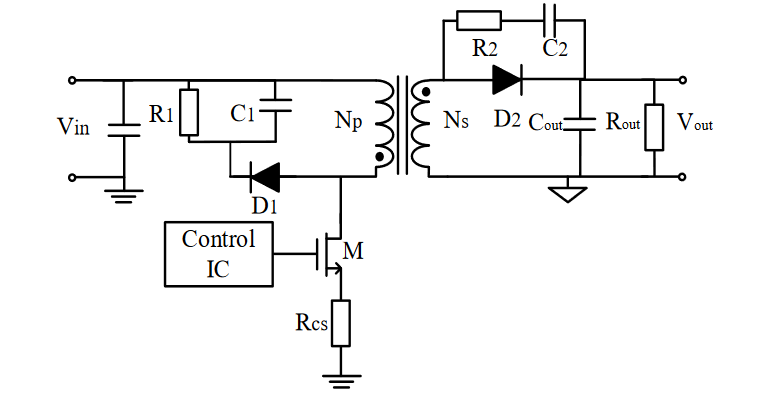
\includegraphics[width=0.6\linewidth]{figures/传统反激式拓扑图.png}
    \caption{传统反激式拓扑图}
    \label{fig:传统反激式拓扑图}
\end{figure}

该变换器系统的拓扑核心结构包括原副边极性相反的变压器、功率开关管、电流采样电阻、副边续流二极管、输出电容和输出负载电阻。功率管开关管的栅极连接变换器芯片的驱动信号,控制功率管的开启和关断;漏端连接在变压器的下边沿,源端连接采样原边电感电流的采样电阻。副边续流二极管的正端连接着变压器副线圈的上边沿,负端连接着输出电容和输出负载电阻。除了核心结构外,拓扑中还包括了RCD尖峰电流吸收电路和二极管保护电路等结构。由于实际的变压器中存在漏感,当功率管在硬开关的条件下被栅极驱动信号关断后,原边电感电流会产生的尖峰信号,加入由电阻、电容和二极管组成的吸收电路可以通过合理消耗漏感的能量来抑制尖峰电流信号的大小;同时考虑到安全性的问题,为了减小副边续流二极管的反向恢复应力,在续流二极管上并联电阻和电容元件,保护续流二极管不会在功率管导通和关断时被烧毁。


\subsection{非对称半桥反激式拓扑结构}

非对称半桥反激式(Asymmetric Half-Bridge Flyback)开关电源变换器拓扑是由传统反激式电路的副边结构和LLC电路的原边结构组合而成,后续简称为AHB反激式。该拓扑结构结合了反激式拓扑和LLC拓扑的优点,既可以利用变压器的漏感实现功率管在全工作范围下的软开关,极大地降低开关损耗,又能通过回收寄生元器件的能量进而提高转换效率,降低变压器的体积,是当前针对中等功率领域极有优势的拓扑结构。

\begin{figure}[htbp] 
    \centering
    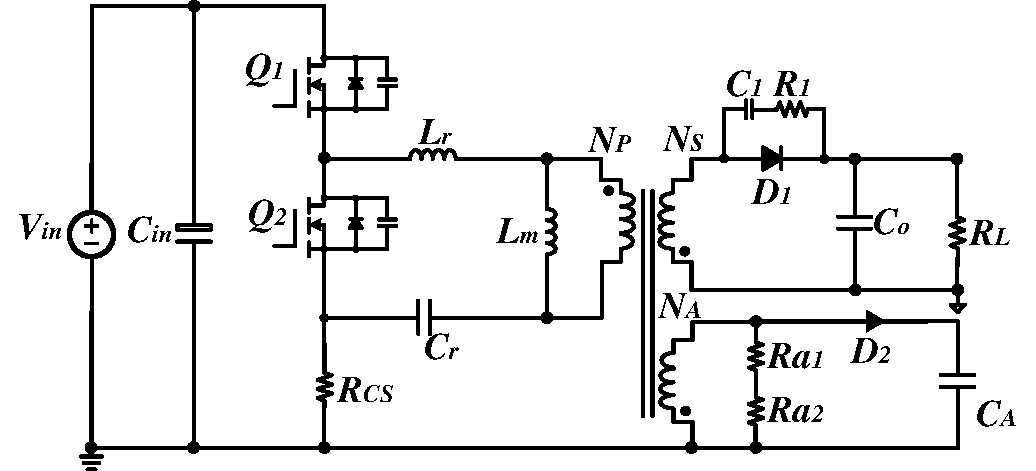
\includegraphics[width=0.8\linewidth]{figures/AHB拓扑图.pdf}
    \caption{AHB反激式拓扑图}
    \label{fig:AHB拓扑图}
\end{figure}

AHB反激式变换器拓扑结构电路如图~\ref{fig:AHB拓扑图}所示。该拓扑的原边电路包括两个功率管开关管$Q_1$和$Q_2$、采样电阻$R_{CS}$、变压器的原边励磁电感$L_m$和漏感$L_r$,以及与变压器和采样电阻串联的谐振电容$C_r$,原边电路类似于LLC变换器,$L_m$、$L_r$$C_r$共同组成串联谐振腔,显示了AHB反激式变换器电路的谐振特性,回收变压器的漏感能量,进而降低变压器体积和提高效率;变压器的副边电路和传统反激式变换器结构的副边相似,由续流二极管$D_1$、输出电容$C_o$和输出负载电阻$R_L$组成,续流二极管两端同样并联电阻$R_1$和电容$C_1$抑制续流二极管的反向恢复应力,此种电路结构可以为变换器系统提供较宽的输出范围。

特别的是该拓扑还包括一个辅助绕组,包括分压电阻$R_{a1}$和$R_{a2}$、续流二极管$D_1$和供电电容$N_A$。该辅助绕组不仅可以通过二极管和电容为变换器芯片提供稳定的供电电压,还可以通过电阻$R_{a1}$和$R_{a2}$分压后为变换器提供额外的电路信息,如检测输出电压的大小和检测副边电流的零电流导通(ZCS)时刻,确保功率管在全工作模式下都实现零电压导通(ZVS)的软开关,从而实现更高的能量转换效率。




\section{工作原理}
\label{sec:工作原理}

非对称半桥反激式开关电源变换器的简化拓扑结构如图~\ref{fig:AHB简化拓扑图}所示。该图中$V_{in}$为直流输入电压;变换器系统中的高低边功率管$Q_1$和$Q_2$的栅极驱动信号分别为占空比为D的HSGD和占空比为1-D的LSGD。每个功率管都包含一个体二极管和寄生电容。谐振电容$C_r$在低边功率管$Q_2$导通时近似为一个恒定的直流源;变压器原边线圈匝数为$N_P$,副边线圈匝数为$N_S$,原边和副边的匝数比为N。输出端D为副边续流二极管,$C_o$为输出滤波电容,R为输出负载电阻。

\begin{figure}[htbp] 
    \centering
    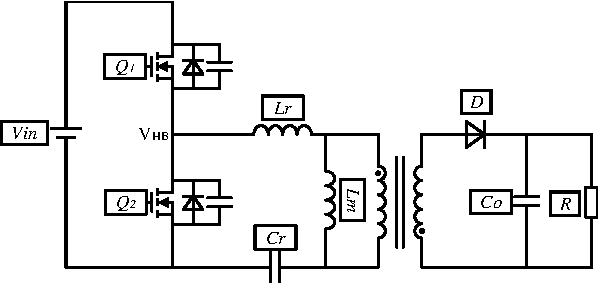
\includegraphics[width=0.8\linewidth]{figures/AHB简化拓扑图.pdf}
    \caption{AHB简化拓扑图}
    \label{fig:AHB简化拓扑图}
\end{figure}

\begin{figure}[htbp] 
    \centering
    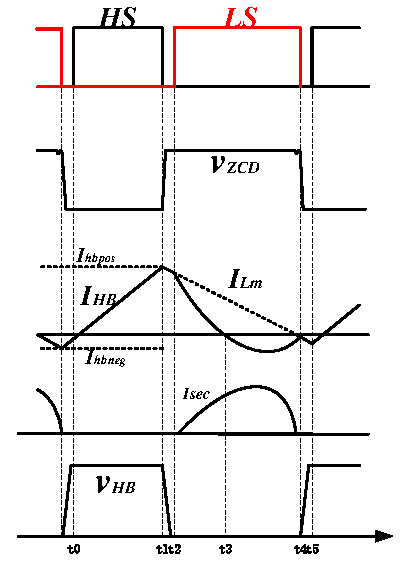
\includegraphics[width=0.8\linewidth]{figures/BCM工作波形图.pdf}
    \caption{AHBF CRM工作模式波形图}
    \label{fig:CRM模式波形图}
\end{figure}
								
非对称半桥反激变换器工作在临界导通模式时的主要工作波形如图~\ref{fig:CRM工作模式波形图}所示。图中从上到下分别是高低边功率管$Q_1$和$Q_2$的电压驱动波形HS和LS、辅助绕组电压分压ZCD引脚电压$V_{ZCD}$的波形、变压器原边励磁电感电流$I_{LM}$和原边电感电流$I_{HB}$的波形、变压器副边电感电流$I_{sec}$的波形,高低边功率管半桥节点电压$V_{HB}$的波形。该控制模式下共分为5个阶段。
						


\begin{figure}[htbp] 
    \centering
    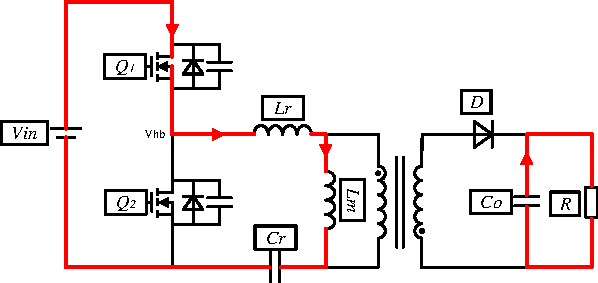
\includegraphics[width=0.8\linewidth]{figures/工作原理1.pdf}
    \caption{阶段1 ($t_0 \thicksim t_1$)}
    \label{fig:工作原理1}
\end{figure}
                
阶段1,$t_0 \thicksim t_1$:此阶段在$t_0$时刻高边功率管$Q_1$完全导通,低边功率管$Q_2$保持关断状态,如图~\ref{fig:工作原理1}所示。半桥节点电压$V_{HB}$等于输入电压$V_{in}$,原边电感电流$I_{HB}$正向流动,输入电压$V_{in}$对原边励磁电感$L_m$、变压器漏感$L_r$和谐振电容$C_r$进行充电,此时原边励磁电感$L_m$、变压器漏感$L_r$和谐振电容$C_r$共同构成谐振回路,由于谐振周期很大,远远大于一个开关周期,其谐振作用在一个开关周期中并不十分明显,因而电感电流近似线性增加。谐振电容$C_r$上的能量持续增加,变压器原边电感电压上正下负,由于变压器的反向作用,副边电感电压上负下正,副边二极管D反向偏置,阻止副边电流$I_{sec}$的产生,输出负载由输出电容提供能量。

在该阶段内,根据回路电压为零和节点电流为零公式,可建立如下方程:
\begin{equation}
    \label{eq:回路电压公式}
    (L_m + L_r)\frac{di_r}{dt} = V_{in} - V_{Cr}  
\end{equation}
\begin{equation}
    \label{eq:结点电流公式}
    V_{Cr}\frac{dV_{Cr}}{dt} = i_r 
\end{equation}

由式\eqref{eq:回路电压公式}和\eqref{eq:结点电流公式}可计算得下式:
\begin{equation}
    \label{eq:Ihb公式1}
    i_{hb}(t) = i_{Lm}(t) = \frac{V_{a}-V_{Cr}(t)}{Z_o}\sin[\omega_o(t-t_0)] + I_{hbneg}\cos[\omega_o(t-t_0)]  
\end{equation}
\begin{equation}
    \label{eq:Vcr_2}
    V_{Cr}(t) =V_{a}-[V_{a}-V_{Cr}(t_0)]\cos[\omega_o(t-t_0)] + {Z_o} I_{hbneg} \sin[\omega_o(t-t_0)]
\end{equation}
其中,特征阻抗值的公式为:
\begin{equation}
    \label{eq:Zo公式}
    Z_o=\sqrt{\frac{L_m+L_r}{C_r}}  
\end{equation}
谐振角频率的公式为:
\begin{equation}
    \label{eq:omega_o公式}
    \omega_o=\frac{1}{\sqrt{C_r(L_m+L_r)}}
\end{equation}
$V_{a}$的公式为:
\begin{equation}
    \label{eq:Vhb公式1}
    V_{a}=V_{in}
\end{equation}

由于谐振角频率$\omega_o$很大,原边电感电流和励磁电流可近似表示为式\eqref{eq:Ihb公式2}:
\begin{equation}
    \label{eq:Ihb公式2}
    i_{hb}(t) = i_{Lm}(t) = I_{hbneg} + \frac{V_{in}-V_{Cr}(t)}{L_m + L_r}(t-t_0)
\end{equation}


\begin{figure}[htbp] 
    \centering
    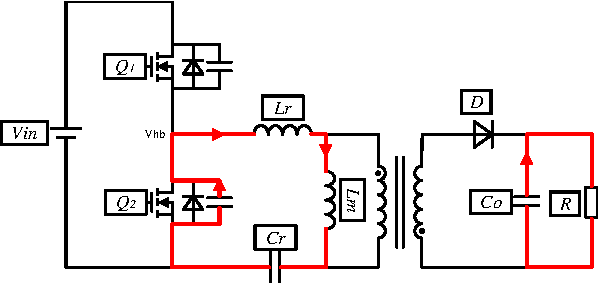
\includegraphics[width=0.8\linewidth]{figures/工作原理2.pdf}
    \caption{阶段2 ($t_1 \thicksim t_2$)}
    \label{fig:工作原理2}
\end{figure}
                
阶段2,$t_1 \thicksim t_2$:此阶段在$t_1$时刻关断高边功率管$Q_1$,同时低边功率管$Q_2$仍保持关断状态,如~\ref{fig:工作原理1}所示,进入功率管死区时间,断开充电路径与 $V_{in}$ 的连接。由于电感电流不能突变,原边电感电流持续正向流动并逐渐减小,对低边功率管$Q_2$的寄生电容进行放电,迫使半桥节点电压$V_{HB}$下降,直到$t_2$时刻低边功率管$Q_2$的体二极管开始导通,$V_{HB}$电压近似为0,为低边功率管的ZVS导通提供准备,此时变压器原边电感两端压降与电容器$C_r$的电压保持一致。输出负载仍由输出电容提供能量。此阶段由于副边二极管仍未被正向偏置,谐振回路未发生变化,特征阻抗值和谐振频率未变仍如式\eqref{eq:Zo公式}和式\eqref{eq:omega_o公式},故原边电感电流和励磁电流仍然相等,但由于$V_{HB}$的近似为0,重新带入式\eqref{eq:Ihb公式1}和式\eqref{eq:Vcr_2}中可将原边电感电流和励磁电感电流公式可近似为式\eqref{eq:Ihb公式3}:
\begin{equation}
    \label{eq:Ihb公式3}
    i_{hb}(t) = i_{Lm}(t) = I_{hbpos} - \frac{N_P}{N_S} \frac{V_o}{L_m + L_r}(t-t_1)
\end{equation}

                
\begin{figure}[htbp] 
    \centering
    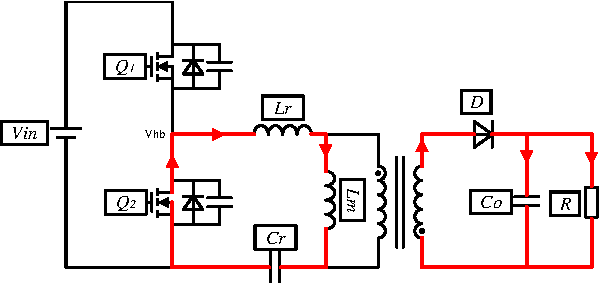
\includegraphics[width=0.8\linewidth]{figures/工作原理3.pdf}
    \caption{阶段3 ($t_2 \thicksim t_3$)}
    \label{fig:工作原理3}
\end{figure}

阶段3,$t_2 \thicksim t_3$:此阶段在t2时刻低边功率管$Q_2$在栅极信号的驱动下顺利在ZVS条件下实现导通,极大地降低了开关损耗,高边功率管$Q_1$仍保持关断状态,如~\ref{fig:工作原理3}所示。功率管中间半桥节点电压$V_{HB}$为零,变压器原边电感极性发生变化,电感电压变为上负下正,经变压器反向后副边电感电压上正下负,副边电感电压等于谐振电容两端电压$V_{Cr}$除以变压器匝数比N,副边二极管D正向偏置自然导通,同时原边励磁电感被输出电压箝位,励磁电感电压的公式为:$V_{Lm}=NV_o$,$L_m$不再参与谐振,谐振电容$C_r$只与变压器的漏感$L_r$发生串联谐振,由于变压器漏感$L_r$和谐振电容$C_r$的谐振周期较小,小于开关周期,可见图中初级侧电感电流呈谐振式持续减小直至正向电流为零。存储在励磁电感中的电能开始通过变压器向副边转移,副边电感电流$I_{sec}$开始逐渐增大。因为副边电流的存在,原边电感电流和励磁电流不再相等,原边电感电流和励磁电感电流的公式分别可表示为式\eqref{eq:Ihb公式4}和\eqref{eq:Ihb公式5}:
\begin{equation}
    \label{eq:Ihb公式4}
    i_{hb}(t) = \frac{\frac{N_P}{N_S}V_o - V_{Cr}(t)}{Z_r}\sin[\omega_o(t-t_2)] + i_{hb}(t_2) \cos[\omega_o(t-t_2)]  
\end{equation}
\begin{equation}
    \label{eq:Ihb公式5}
    i_{Lm}(t) = i_{hb}(t_2) - \frac{N_P}{N_S} \frac{V_o}{L_m}(t-t_2)
\end{equation}
其中,特征阻抗值的公式为:
\begin{equation}
    \label{eq:Zr公式}
    Z_r=\sqrt{\frac{L_r}{C_r}}  
\end{equation}
谐振角频率的公式为:
\begin{equation}
    \label{eq:omega_r公式}
    \omega_r=\frac{1}{\sqrt{C_r L_r}}
\end{equation}
由于励磁电感电流等于原边电感电流和经变压器反射后的副边电流之和,如式\eqref{eq:Ihb公式6}所示,将式\eqref{eq:Ihb公式4}和\eqref{eq:Ihb公式5}带入其中可求得副边电流公式\eqref{eq:Isec公式1}:
\begin{equation}
    \label{eq:Ihb公式6}
    I_{Lm} = I_{HB} + \frac{N_P}{N_S}I_{sec}
\end{equation}
\begin{equation}
    \label{eq:Isec公式1}
    i_{sec}(t) 
    %&= \frac{N_P}{N_S}[i_{Lm}(t) - i_{hb}(t)] \\ &
    = \frac{N_P}{N_S} i_{hb}(t_2) \{  1 - \cos[\omega_r(t-t_2)]\}  - \frac{N_P^2}{N_N^2} \frac{V_o}{L_m} (t-t_2)
    - \frac{\frac{N_P^2}{N_S^2} V_o - V_{Cr}}{Z_r} \sin[\omega_r(t-t_2)]
\end{equation}
随着副边电流的逐渐增大,原边电感电流在$t_3$时刻正向降低为零,该阶段结束。



\begin{figure}[htbp] 
    \centering
    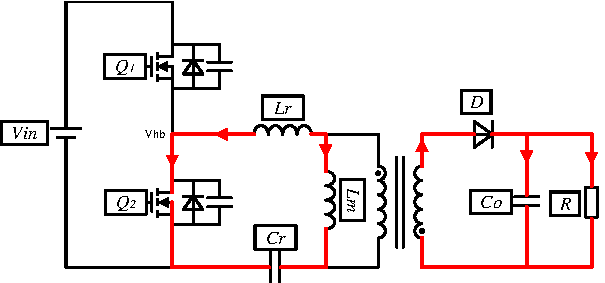
\includegraphics[width=0.8\linewidth]{figures/工作原理4.pdf}
    \caption{阶段4 ($t_3 \thicksim t_4$)}
    \label{fig:工作原理4}
\end{figure}

阶段4,$t_3 \thicksim t_4$:此阶段高低边功率管$Q_1$和$Q_2$仍保持上一阶段状态,在$t_3$时刻原边电感电流正向降低为零,开始负向流动并持续增大,如~\ref{fig:工作原理4}所示。此时谐振电容$C_r$和励磁电感$L_m$共同为副边提供能量。同时,励磁电感电流也逐渐降低至与原边电感电流相等的值,如~\ref{fig:CRM模式波形图}中$t_4$时刻所示,此时励磁电感能量全部退磁完成,不再为副边提供能量,副边电感电流$I_{sec}$降低为零,辅助绕组电感电压分压$V_{ZCD}$波形上出现高频谐振,这是因为副边二极管寄生电容和变压器漏感发生的谐振现象,这一反映励磁电感退磁完成的高频谐振波形可以作为判断低边功率管关断的关键信号,故在$t_4$时刻低边功率管在栅极信号驱动下开始关断。

\begin{figure}[htbp] 
    \centering
    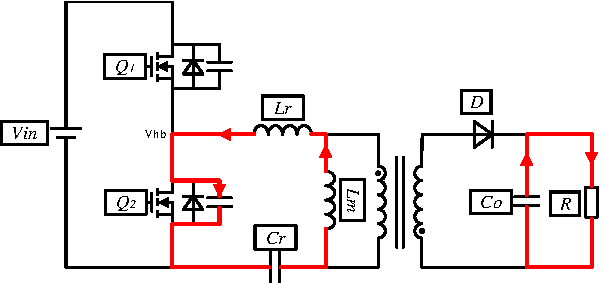
\includegraphics[width=0.8\linewidth]{figures/工作原理5.pdf}
    \caption{阶段5 ($t_3 \thicksim t_4$)}
    \label{fig:工作原理5}
\end{figure}
                
阶段5,$t_4 \thicksim t_5$:此阶段高低边功率管都保持关断状态,再次进入功率管的死区时间,如~\ref{fig:工作原理5}所示。由于励磁电感内存储的能量已全部传递到变压器副边,副边二极管在ZCS条件下自然关断,输出电压不再箝位励磁电感,励磁电感和变压器漏感共同和谐振电容串联谐振,特征阻抗值恢复为$Z_o$,谐振角频率恢复为$\omega_o$,谐振周期远远大于开关周期,原边电感电流和励磁电感电流如\eqref{eq:Ihb公式2}所示,因为电感电流无法进行突变,电感电流仍负向流动,对低边功率管$Q_2$寄生电容进行充能,逐渐拉高半桥节点电压$V_{HB}$,直至$t_5$时刻半桥节点电压$V_{HB}$被高边功率管$Q_1$中的体二极管钳位,$V_{HB}$近似等于输入电压,电路达到开启高边功率管$Q_1$的ZVS条件,至此,一个周期结束。

								
%阶段1,$t_0$-$t_1$:此阶段在$t_0$时刻高边功率管$Q_1$完全导通,低边功率管$Q_2$保持关断状态,进入功率%管死区时间。



\section{开关电源的工作模式}
\label{sec:dataset-build}

开关电源工作模式分为三种,包括连续导通模式(CCM)、边界导通模式(BCM)以及断续导通模式(DCM),本文设计分别采用了断续导通模式(DCM)和边界导通模式(BCM)。以下是对三种工作模式的具体研究情况。

\subsection{CCM连续导通模式}
对于非对称半桥反激式开关电源变换器而言,不同于传统的反激式开关电源变换器,连续导通模式是指,当系统给出功率开关管的下一周期导通信号时,变压器原边电感电流和励磁电感电流未重合,变压器励磁电感中的能量还没有完全退磁转移到次级侧负载,紧接着又从输入端开始继续获取能量。

\begin{figure}[htbp] 
    \centering
    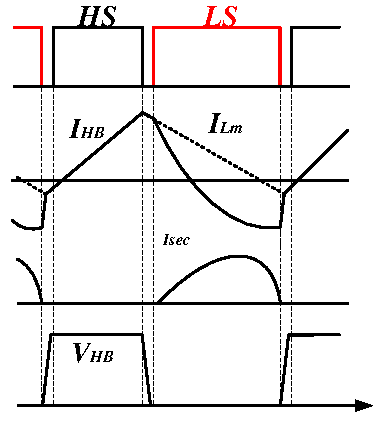
\includegraphics[width=0.8\linewidth]{figures/CCM模式.pdf}
    \caption{CCM工作模式波形图}
    \label{fig:CCM工作模式波形图}
\end{figure}

非对称半桥反激式开关电源变换器在连续导通模式下的波形如下图所示,tHSon是高边功率管HS的导通时间,tLSon是低边功率管LS的导通时间,$V_{HB}$是高低边功率管的中间节点电压,VCr是初级侧谐振电容的两端电压差,Ihb是初级侧电感电流,ILm是励磁电感电流,Isec是次级侧电感电流。

当高边功率管导通时,输入电压的能量在变压器励磁电感和谐振电容中积累,当高边功率管关断时,励磁电感和谐振电容中的能量经由副边绕组传递到输出端。当下一周期高边功率管导通再次开始励磁时,变压器励磁电感和谐振电容中储存的能量还未完全退磁传递到副边绕组的工作模式就是CCM模式。

\iffalse
在输入输出电压稳定运行期间,对励磁电感应用伏秒平衡原理,能够得到输入电压、输出电压和占空比D之间的关系。在tHSon内,励磁电感两端电压为输入电压减去谐振电容电压Vcr;在tLSon内,励磁电感两端电压为谐振电容电压Vcr,由此可得式\eqref{eq:CCM_1}:
\begin{equation}
    \label{eq:CCM_1}
    D\times(V_{in}−V_{cr\_avg})=(1−D)\times V_{cr\_avg}
\end{equation}
\begin{equation}
    \label{eq:Vcr_1}
    V_{cr\_avg}=N \times V_o\times\frac{L_m}{L_m+L_r}
\end{equation}
其中$V_{cr\_avg}$是谐振电容Cr上的平均电压,它等于输出电压经变压器原边励磁电感和漏感分压后乘以匝数比N。

对式\eqref{eq:CCM_1}和\eqref{eq:Vcr_1}进行整理可得式\eqref{eq:CCM_3}:
\begin{equation}
    \label{eq:CCM_3}
    V_o=D \times \frac{V_{in}}{N} \times\frac{L_m}{L_m+L_r}  
\end{equation}

根据式\eqref{eq:CCM_3}可知输出电压由占空比D、输入电压、变压器匝数比N、变压器励磁电感和漏感决定,与负载恒和频率无关。由于Lr对Lm而言非常小可以忽略不计,式\eqref{eq:CCM_3}可化简为式\eqref{eq:CCM_4}:
\begin{equation}
    \label{eq:CCM_4}
    V_o=D \times \frac{V_{in}}{N}  
\end{equation}
\fi
\subsection{DCM断续导通模式}

\begin{figure}[htbp] 
    \centering
    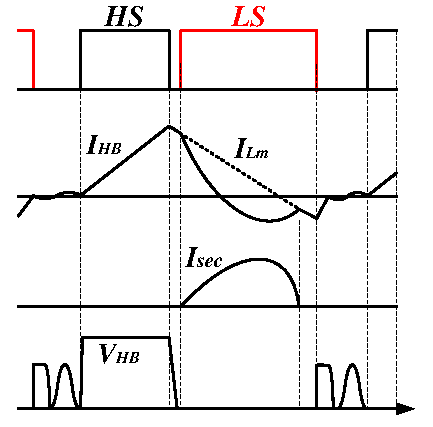
\includegraphics[width=0.8\linewidth]{figures/DCM模式.pdf}
    \caption{DCM工作模式波形图}
    \label{fig:DCM工作模式波形图}
\end{figure}

开关电源工作在连续导电模式(CCM)下时,当开关管导通的一瞬间,变压器就 立刻响应,此时变压器的电流为非零电流,在任意一个周期,变压器都会储存能量。 连续导电模式(CCM)是反激变换器在固定频率下工作的一种典型工作方式[29]。图 2.8 为连续导电模式下开关电源工作时原边电流和副边电流(即二极管上的电流)波 形。副边电流的每个周期从一开始就储存能量结束时不归为零,这就要求在各个周期 中能量都被变压器储存,并且能量可以跨周期存在。因此,当负载电流改变时,变压 器中储存的能量也相应随之改变。

\subsection{CRM临界导通模式}

\begin{figure}[htbp] 
    \centering
    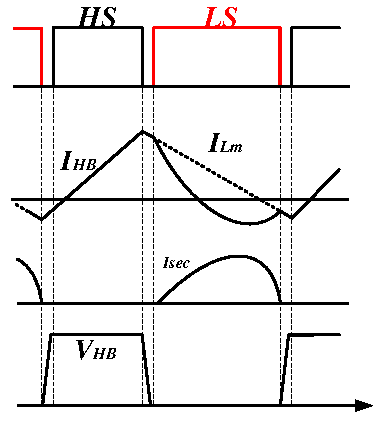
\includegraphics[width=0.8\linewidth]{figures/CRM模式.pdf}
    \caption{CRM工作模式波形图}
    \label{fig:CRM工作模式波形图}
\end{figure}

临界导通模式(Critical Conduction Mode,CRM)的工作原理和它的名称一样,是一种介于连续导通模式和断续导通模式中的特殊的工作模式。不同于其他开关电源拓扑,在非对称半桥反激式变换器的CRM工作模式下,原边电感电流和励磁电感电流重合的瞬间功率管进行切换动作,同时副边电感电流在此时恰好下降到零电流,变压器原边励磁电感内储存的能量刚好全部传递到副边,并经过短暂的死区时间后,开启下一个开关周期。

临界导通模式不仅实现了最大的能量传递,还有助于实现非对称半桥反激式变换器的ZCS关断,减小关断损耗,并相较于DCM的ZCS,近似没有的死区时间极大的降低了导通损耗,提高变换器的效率。CRM工作模式的典型波形如图~\ref{fig:CRM工作模式波形图}所示。




%\subsection{CRM临界导通模式}




\section{开关电源的脉宽调制方式}
开关电源通过调节开关管控制信号的导通关断时间来改变信号占空比由此达到稳定输出电压或输出电流的目的,根据改变占空比方式的不同将会得到不同的开关电源调制方式,本节将分别介绍脉冲宽度调制(PWM)、脉冲频率调制(PFM)、脉冲跳周期调制(PSM)以及脉冲宽度频率调制(PWM-PFM)。

\subsection{PWM调制方式}
PWM调制的原理是指在功率管开关频率不变的情况下通过控制功率管管的导通时间来改变占空比的大小进而维持输出电压或输出电流的稳定,即定频调宽。这是开关电源变换器中最常用的一种调制方式,常见的PWM脉宽调制系统如下图所示,是将输出电压通过电阻串进行分压后产生的输出反馈信号Vfb与参考电压在误差放大器中进行比较,产生误差放大信号Vea,Vea再与频率固定的三角波信号在PWM比较器中比较,生产占空比不同的PWM控制信号来控制功率管的导通和关断,其中电压模的锯齿波信号由固定电路给定,电流模的锯齿波信号由原边电流采样电阻上的电压处理得到。

\begin{figure}[htbp] 
    \centering
    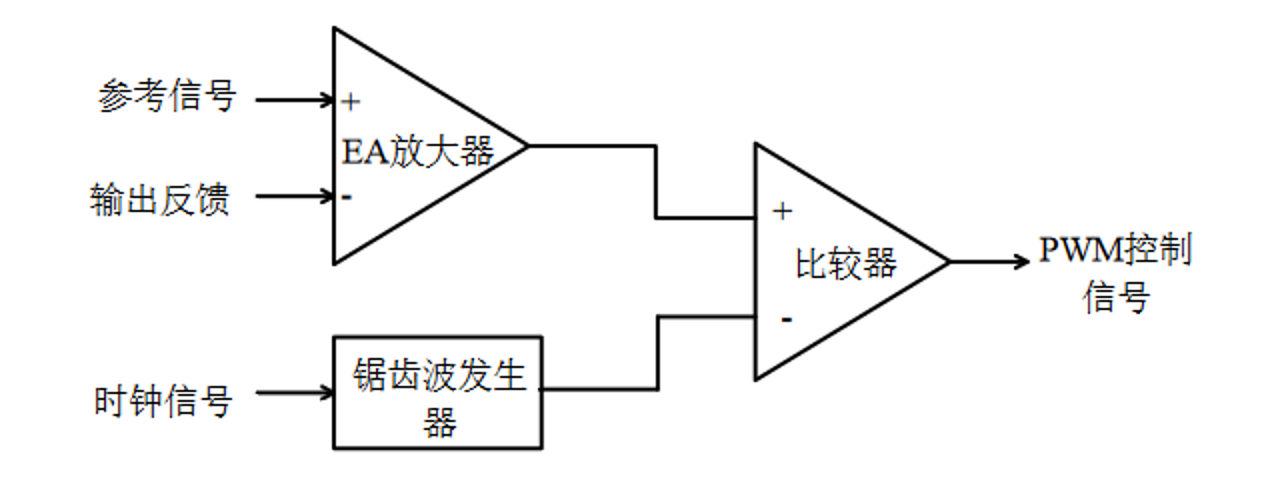
\includegraphics[width=0.8\linewidth]{figures/PWM调制1.png}
    \caption{PWM调制原理图}
    \label{fig:PWM调制1}
\end{figure}

当输出负载电流变大,输出负载会从输出电容中抽取能量,输出电压Vo变小,相应Vfb也变小,因此误差放大信号Vea增大,Vea与锯齿波信号比较后得到的脉冲宽度就会增大,导致PWM控制信号的占空比增大,将更多的能量在下一个周期中传递到副边电路维持输出电压的稳定。PWM调制作为最常用的调制方式,具有控制结构简单易于设计和实现、输出电压纹波小,动态响应快,线性度高,频率特性好等优点。但PWM调制由于频率固定,其更适用于重载情况下,因为不论输出负载大小如何,每个周期功率管都会进行导通关断操作,导致当输出负载处于空载和轻载情况下造成更多的开关损耗,电路的能量转换效率很低。

\subsection{PFM调制方式}
PFM调制的原理是指在功率管导通时间不变的情况下通过控制功率管的开关频率来改变占空比的大小进而维持输出电压或输出电流的稳定,即定宽调频。

常见的PWM脉宽调制系统如下图所示,同样是将输出电压通过电阻串进行分压后产生的输出反馈信号Vfb与参考电压在误差放大器中进行比较,产生误差放大信号Vea,不同于PWM调制,PFM调制的Vea信号输入到脉冲调制器中产生时钟信号CLK控制功率管的导通;功率管导通时长由原边电流采样电阻上的电压Vcs与给定的参考电压Vcsref比较所得的关闭信号控制。当脉冲调制器中
\subsection{PSM调制方式}
利用恒频恒宽进行调节的方式称为脉冲跳周期调制,这样一种全新的控制模式被 应用于开关功率变换器,当使用 PSM 调制时脉冲的宽度和频率保持恒定,这些脉冲 作为开关管的输入信号,所需要周期的个数会由负载的大小来进行决定。当参考电压 大于输出电压,恒定频率和宽度的时钟控制信号允许功率开关管在该周期中工作,当参考电压小于输出电压时,该周期将会被开关管忽略。PSM 调制模式其效率并不取决于输出功率,当负载发生变化时效率仍然保持恒 定,脉冲跳周期调制模式的优点是轻负载时的转换效率比脉冲宽度调制模式高、抗干扰能力强、静态功耗低;跳过一些工作周期后,会带来很大的输出电压波纹、线性调 整率变差、系统的有效频率降低等缺点。
\subsection{PWM+PFM调制方式}
PWM-PFM 是一种将 PWM 调制方法与 PFM 调制方法相结合的混合调制方法。 由上文分析可知,在高负载的情况下,PWM 调制方式效率更高,输出纹波小,开关频率固定,开关周期固定,因此针对 PWM 模式的噪声滤波器设计比较简单;但在负载较轻的情况下效率会降低,而 PFM 调制方法在轻载下频率会降低因而会有更高的 效率。PWM-PFM 混合调制方法具备 PWM 调制方法和 PFM 调制方法共同的优点。 PWM-PFM 混合调制模式兼具两种调制模式的优点,它既可以改变开关管控制信号的 频率,又可以改变控制信号脉冲宽度。在不同的负载情况下采用不同的方法使开关电 源的效率始终高于不考虑负载变化的情况,但混合调制方法对应的电路设计非常复杂,不同的控制回路需要设计采用不同的补偿结构。

\section{开关电源的环路控制方式}
为了使电路的输出端可以连接不同大小的负载,需要在输出电路中加入反馈电路 使输出达到稳定的状态,从而整个系统也能够继续稳定地工作。反馈环路是指输出端 采样到运放的输出端,被控对象是指运放输出到系统输出,在开关电源的设计中,反馈电路的性能会对开关电源的精度和总体性能产生巨大影响。因此,良好反馈回路的设计是开关电源系统开发的关键,开关电源既可以用电压也可以用电流控制,下 面对这两种模式的工作原理进行详细分析。

\subsection{电压控制模式}
电压控制环路属于单环路控制方式,只包含一个和输出电压信号相关的电压反馈回路,具有结构简单、设计容易和抗干扰能力强等优点。电压控制模式的典型电路如~\ref{fig:电压工作模式电路图} 所示,主要由误差放大器、振荡器、比较器、SR锁存器和驱动电路等组成。误差放大器的负输入端是辅助绕组采样输出电压后通过分压电阻串 R1、R2 得到的分压电压,正输入端是参考电压Vref,误差放大器通过放大分压电压和参考电压的差异生成误差放大信号VEA。当输出负载变化时会导致输出电压上冲或下冲,该变化会引起VEA的上下波动,因此VEA可以反映输出负载的变化,锯齿波信号与VEA通过比较器比较后即可在不同输出负载的情况下调节SR锁存器的复位时间,进而改变驱动模块生成的脉冲宽度大小。当负载电流减小,分压电压大于参考电压,误差电压信号VEA降低,从而VEA通过比较器和锯齿波电压信号比较后生成的输出信号更早得控制SR锁存器复位,驱动模块产生的控制高边功率管导通信号的脉宽变窄,降低对变压器副边的能量传递,将输出电压逐渐降低到标准范围,维持输出电压的稳定。

\begin{figure}[htbp] 
    \centering
    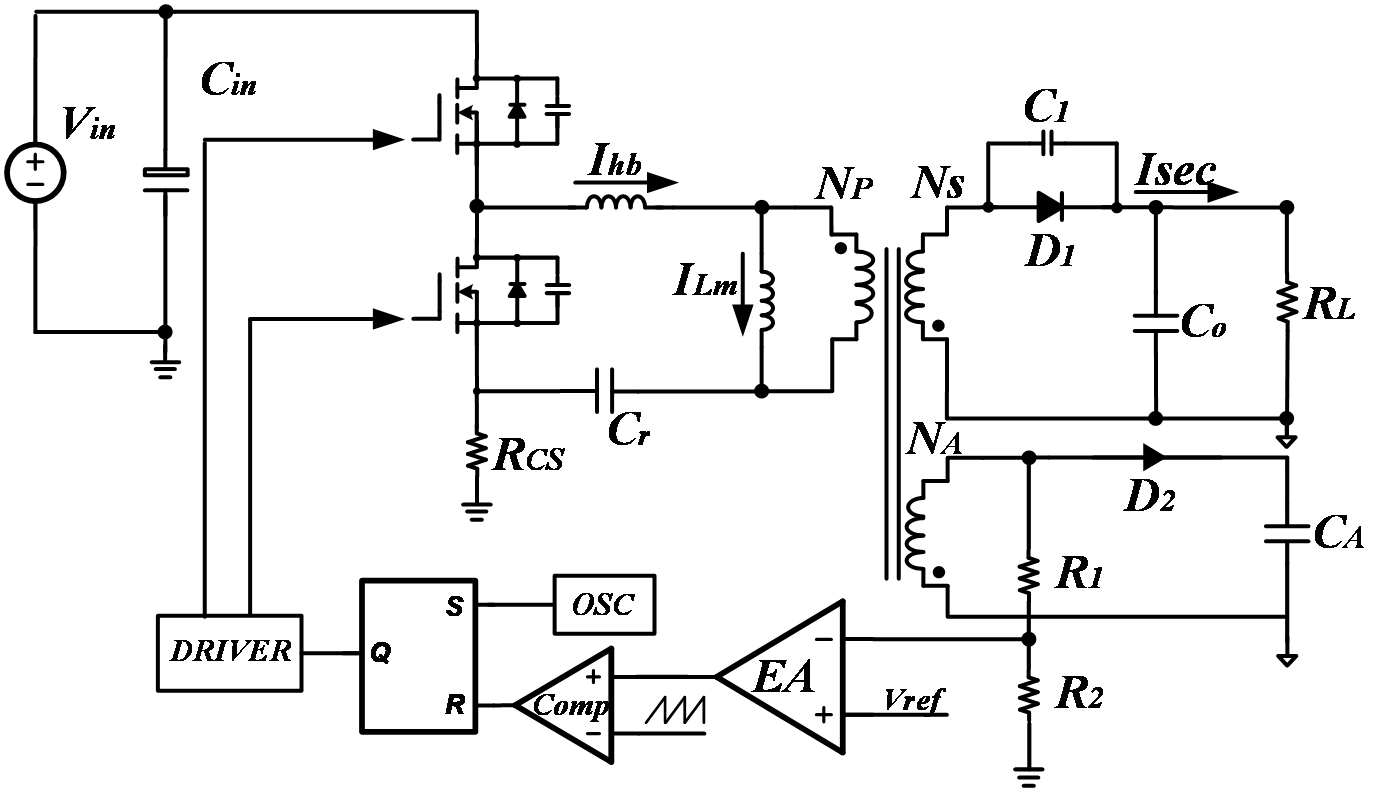
\includegraphics[width=0.8\linewidth]{figures/电压工作模式电路图.png}
    \caption{电压工作模式电路图}
    \label{fig:电压工作模式电路图}
\end{figure}

电压控制环路虽然结构简单且易于控制,但是由于只有一个电压环路,故只有当输出电压发生变化之后才会影响功率管的导通和关断时间,开始进行闭环负反馈动态调节,当输入电压产生干扰时,原边电感电流的上升斜率发生变化,会影响原边励磁电感的储能,但电压环路的控制和调节不会立即发生作用,而是在延迟一段时间之后才会起作用,系统整体的动态响应就会变差,输出电压产生很大的上冲和下冲现象。

\subsection{电流控制模式}
\label{sec:电流控制模式}
电流控制环路属于多环路控制方式,典型电路图如~\ref{fig:电流工作模式电路图}所示,包含一个电压环路和一个电流环路,电压环路和电压控制环路相同,采样输出电压信号用于生成误差放大信号;电流环路则是实时采样功率管的电流作为反馈电流,用采样电阻将电流转换为采样电压替代电压控制模式中的锯齿波信号,同误差放大信号VEA进行比较。

\begin{figure}[htbp] 
    \centering
    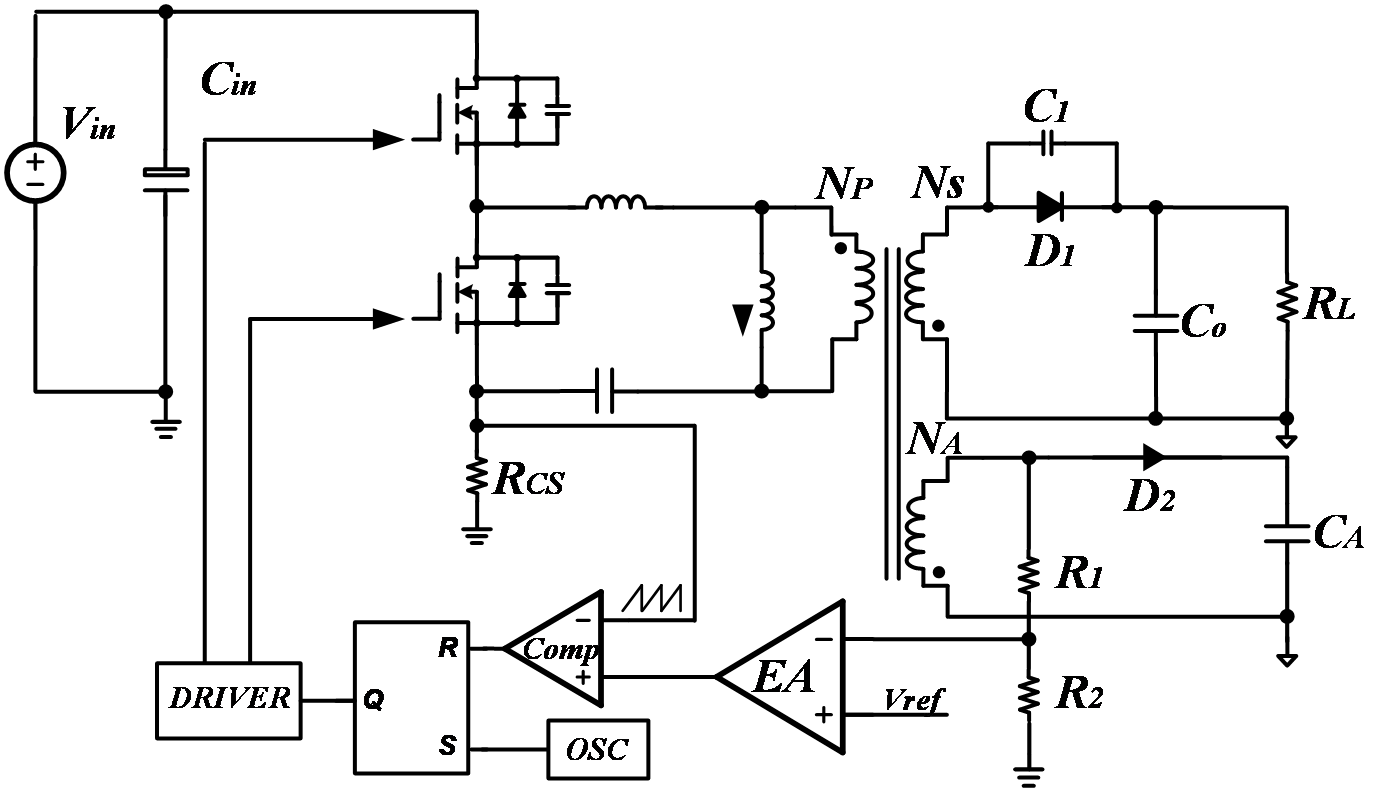
\includegraphics[width=0.8\linewidth]{figures/电流工作模式电路图.png}
    \caption{电流工作模式电路图}
    \label{fig:电流工作模式电路图}
\end{figure}

相比于电压控制模式对输入电压信号的不敏感,电流控制模式对输入输出信号都可以进行反馈,输入电压信号的变化会影响功率管导通时刻的电流斜率,通过采样电阻后产生一个随输入电压变化而变化的锯齿波信号,当输入电压发生扰动时,反馈环路可以直接响应改变功率管导通时间,而不需要等待输出电压信号发生相应波动后改变VEA的大小再影响功率管导通时间,极大地提高了系统整体的动态响应时间。但由于电流控制模式包含两个反馈环路,增大了电路结构的设计复杂度,另外,当驱动信号的占空比大于 50\%时,电路中不可避免地会出现次谐波振荡, 这需要增加额外的斜坡补偿电路来解决,一定程度上,也增加了应用难度。

 
\section{开关电源的反馈方式}
反激式开关电源变换器电路为保证输出电压稳定,进行闭环回路控制,需要对输出电压信号进行采样,并通过不同的方式将其反馈到变换器芯片进行逻辑处理。反激式开关电源变换器根据反馈结构的不同分为原边反馈(PSR)和副边反馈(SSR)两种反馈方式。其中原边反馈是通过辅助绕组对副边输出电压信号进行检测采样,副边反馈是通过 TL431 稳压模块和光耦模块组成的反馈系统对输出电压信号进行检测采样。

\subsection{原边反馈电路}
非对称半桥反激式变换器的原边反馈电路拓扑结构如~\ref{fig:原边反馈电路电路图}所示。

\begin{figure}[htbp] 
    \centering
    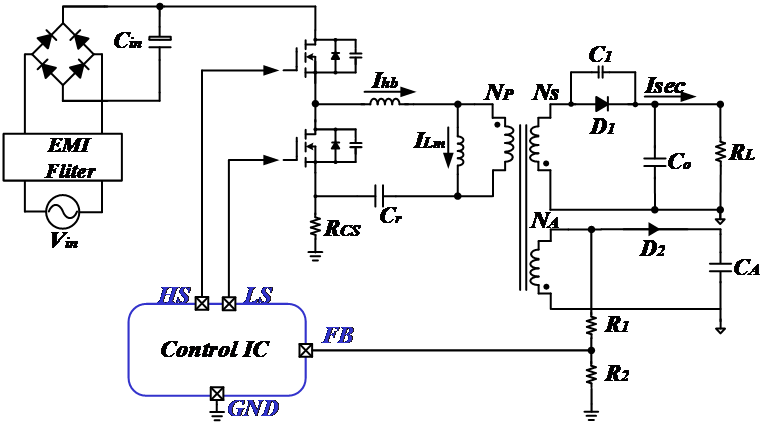
\includegraphics[width=0.8\linewidth]{figures/原边反馈电路图.png}
    \caption{原边反馈电路电路图}
    \label{fig:原边反馈电路电路图}
\end{figure}

原边反馈电路依靠辅助绕组采样输出电压,隔离变压器的特性是原边绕组、副边绕组和辅助绕组两端的电压相互成比例,原边绕组和辅助绕组电压极性相反,副边绕组和辅助绕组电压极性相同,因此辅助绕组电感电压值等于输出电压乘以副边绕组和辅助绕组的匝数比。在非对称半桥反激式开关电源系统中,在高边功率管导通阶段辅助绕组电感电压绝对值正比于原边绕组电感电压;低边功率管导通阶段辅助绕组检测副边绕组电感电压。辅助绕组电感电压VA经过R1和R2分压后得到原边反馈电压VFB送入变换器控制IC中参与闭环环路控制用以维持在负载变化情况下输出电压的稳定性。VA和VFB的电压值由式\eqref{eq:辅助绕组电压}和式\eqref{eq:VZCD公式}所示:
\begin{equation}
    \label{eq:辅助绕组电压}
    V_A = \frac{N_A}{N_S}\times(V_o + V_{D1})
\end{equation}
\begin{equation}
    \label{eq:VZCD公式}
    V_{FB} = V_A\times\frac{R_{a2}}{R_{a1}+R_{a2}}=\frac{N_A}{N_S}\times(V_o + V_{D1})\times\frac{R_{a2}}{R_{a1}+R_{a2}}
\end{equation}

\subsection{副边反馈电路}
非对称半桥反激式变换器的副边反馈电路拓扑结构如~\ref{fig:副边反馈电路电路图}所示。

\begin{figure}[htbp] 
    \centering
    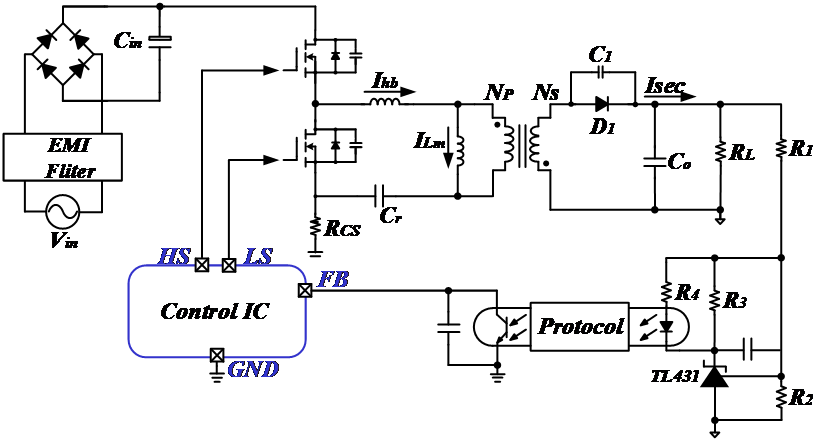
\includegraphics[width=0.8\linewidth]{figures/副边反馈电路图.png}
    \caption{副边反馈电路电路图}
    \label{fig:副边反馈电路电路图}
\end{figure}

副边反馈电路主要通过变压器副边侧基于TL431的反馈系统采集输出电压信号,该反馈系统包括输出电压分压电阻串R1和R2、TL431稳压模块、光电耦合器以及用于补偿的电容电阻。输出电压Vo通过分压电阻串R1和R2分压后送入TL431稳压模块中与其中自带的2.5V参考电压比较后产生一个误差信号,该误差信号经过光电耦合器,将电信号转化为光信号传输到变压器原边后再转化为电信号,实现变压器原副边电气隔离,TL431稳压模块可类似为一个误差放大器,通过额外的电阻电容组成的补偿网络对TL431输出的误差信号进行补偿,相当于集成在原边反馈系统变换器中的反馈网络移到了片外,可以根据不同的情况通过改变电阻电容的方式进行更精确的调节,将包含输出电压和负载电流信息的反馈电压VEA传递给变换器中。

相比于副边反馈电路,原边反馈电路由于不需要额外的外围电路,通过将反馈电压VFB输入变换器芯片内与参考电压在误差放大器中比较后输出误差放大信号Vea用于反馈环路的调节,具有较高的集成度,极大地节省了芯片外围电路板的面积,但由于副边绕组的电感电压并不完全等于输出电压,而是等于输出电压和副边续流二极管导通电压之和,导致副边绕组电感电压还可能受到负载电流和温度等因素的影响,且辅助绕组和副边绕组间存在的不匹配的情况,也将导致实际反馈电压值异于式(2-)的计算值,故而相比于副边反馈,原边反馈的采样准确性明显更低,为了消除这些误差,原边反馈电路需要添加更多的补偿电路极大增大电路设计复杂度,增大芯片的面积和功耗。因此副边反馈电路广泛应用于工业届,几乎所有的中等功率消费类电源都使用副边反馈系统。



 

\section{小结}


本章首先对反激式电源拓扑的工作原理进行了研究,从传统反激式变换器的拓扑结构到非对称半桥反激式变换器的拓扑结构;
然后结合非对称半桥反激式系统中关键信号波形和工作状态对该其工作原理进行了具体的分析和理论推导;
又分别针对CCM、DCM和CRM三种工作模式进行了阐述;
接着简单介绍了PWM、PFM、PSM和PWMFM四种脉宽调制技术;
再描述了开关电源中的两种环路控制方式,即电压控制模式和电流控制模式,对它们的工作原理以及优缺点进行了说明比较;
最后对反激式变换器最常使用的原边反馈和副边反馈两种反馈方式的工作方式进行介绍和分析。


















\chapter{系统设计}
本章给出了本文设计的非对称半桥反激式变换器系统的性能和设计指标。 首先给出了本文设计的AHB变换器的性能指标,介绍了控制芯片的内部原理图。此外, 为了提高系统的转换效率,分析了反激式变换器的主要损耗,总结了影响系统损耗的主要因素。根据损耗分析的结果,设计了多模式的控制方案,通过系统的带载情况来调节变换器的开关频率和原边的峰值电流值,从而降低系统的损耗,实现系统的整体效率的提升。另外,为了进一步提高系统的转换效率,针对性的提出了两种关键技术,分别用以降低功率管开关损耗和变压器的传导损耗。除此之外,为了降低系统的待机功耗,设计了空载下的突发工作模式。最后为了保证变换器能够稳定的运行,设计了副边反馈网络的二阶补偿结构,并对系统进行了稳定性仿真。


\section{外部电路结构}
本文设计的非对称半桥反激式开关电源变换器的外部电路结构如图所示,包括输入整流回路和反馈回路,为了提高反馈精度,反激回路采用副边反馈结构,通过TL431和光耦模块直接对输出电压进行采样产生误差信号反馈给变换器芯片来为稳定输出电压。

输入回路包扩输入整流滤波和片外启动电路两部分,输入整流滤波由四个二极管和电容Cdc组成,将从电网传递进来的交流信号Vac经过整流滤波后转换为直流输入信号Vdc,此输入信号是一个直流的高压,无法直接为变换器芯片进行供电,通过电阻R1和R2分压后给变换器芯片供电,当其超过片内欠压锁定电路的最低电压后芯片开始工作,随着芯片控制高低边功率管的来回通断,辅助绕组能量积攒到一定程度后,二极管D2导通,对电容Cvdd进行充电,产生变换器输入电压Vdd,代替输入信号Vdc的分压信号稳定地为变换器芯片电源端进行供电。


\section{系统架构}

\subsection{芯片特点和设计指标}

• 支持宽输入电压范围

• 支持宽输出电压范围

• 高效多模式控制

• 轻载低功耗模式

• 全电压和负载条件下支持零电压导通

\begin{table}[htbp]
    \caption{控制芯片的引脚定义}
    \label{tab:控制芯片的引脚定义}
    \centering
    \belowrulesep=0pt  %防止竖线不连续
    \aboverulesep=0pt  %防止竖线不连续
        \begin{tabular}{c|c|c}
            \toprule
            引脚标号 & 名称 & 功能  \\
            \midrule
            1 & EN   & 使能端                                              \\  \midrule
            2 & VDD  & 变换器芯片内部供电端                                 \\  \midrule
            3 & HSGD & 半桥变换器高边功率管的栅极驱动器,控制高边功率管的通断  \\\midrule  
            4 & LSGD & 半桥变换器高边功率管的栅极驱动器,控制低边功率管的通断  \\\midrule  
            5 & ZCD  & 辅助绕组分压采样端                                    \\  \midrule
            6 & CS   & 变压器原边峰值电流采样端                               \\ \midrule
            7 & VS   & 输入电压分压端                                        \\  \midrule
            8 & GND  & 变换器芯片接地端                                      \\  \midrule
            9 & HB   & 功率管半桥中间节点端                                   \\ 
              
            \bottomrule
        \end{tabular}
\end{table}

\subsection{芯片内部结构}
图~\ref{fig:芯片内部结构图}给出了芯片内部结构架构,该架构包括电源模块、峰值电流控制模块、 退磁检测模块、前沿消隐模块、精确谷底导通模块、谷值锁定模块、前沿消隐(LEB)、退磁时间逐步逼近模块、模式选择模块、逻辑控制模块和驱动等主要模块,每个模块的功能定义如下:

\begin{figure}[htbp] 
    \centering
    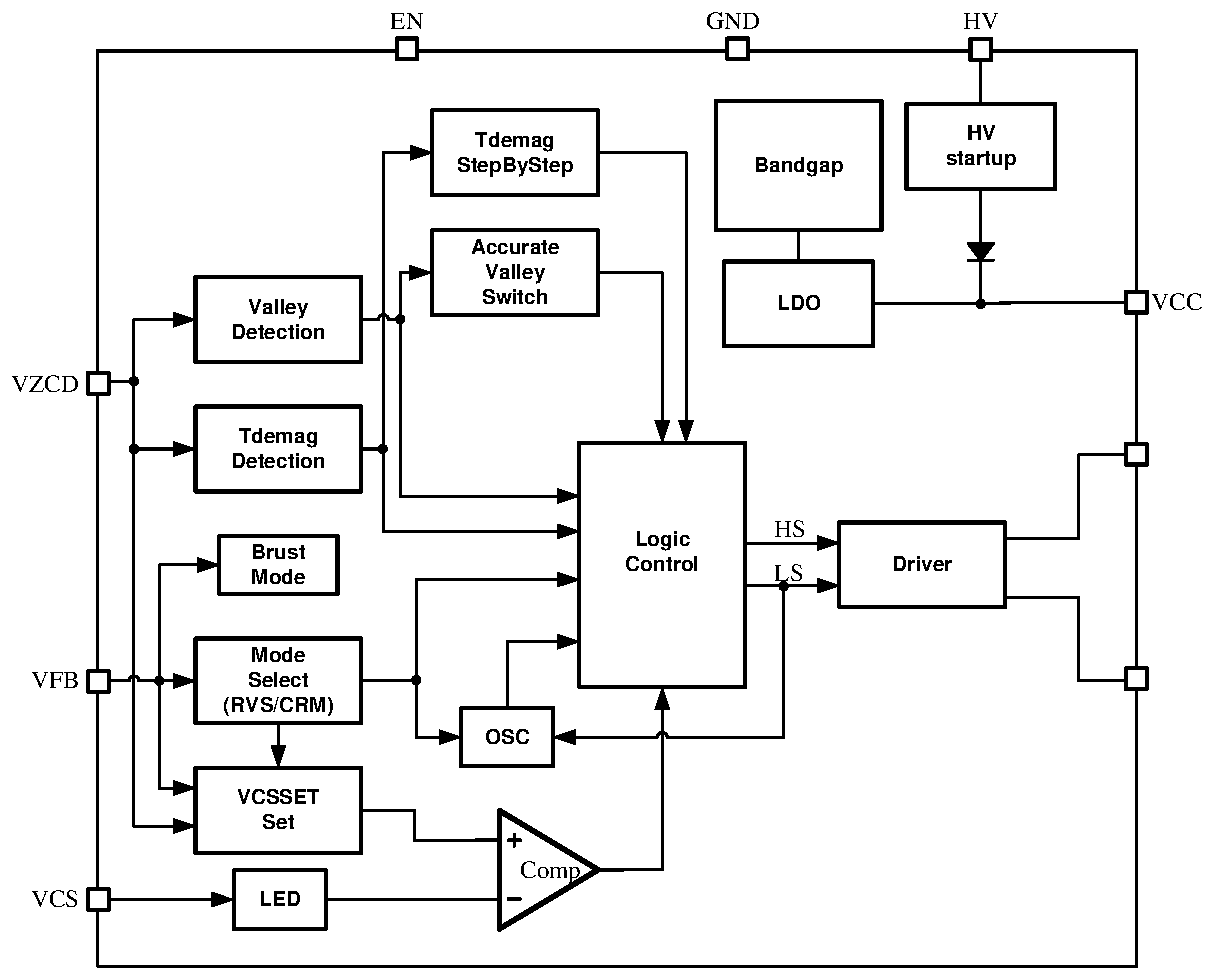
\includegraphics[width=0.8\linewidth]{figures/芯片内部结构图.pdf}
    \caption{芯片内部结构图}
    \label{fig:芯片内部结构图}
\end{figure}

\textbf{电源模块}:电源模块主要包括芯片的欠压锁定电路、带隙基准和降压电路等,该模块的主要作用是为芯片内部各个模块提供稳定的供电电压和各种不受PVT影响的精确偏置电压信号。

\textbf{峰值电流控制模块}:峰值电流控制模块通过对片外副边反馈信号$V_{FB}$和辅助绕组分压信号$V_{ZCD}$进行配置补偿后,产生对应的峰值电流信号Vcspeak,用于和采样电阻上的采样电压信号Vcs进行比较控制高边功率管的导通和关断;该模块的主要功能是为了满足非对称半桥反激式开关电源变换器的宽输出范围下产生相对应的峰值电流信号Vcspeak,防止副边反馈信号$V_{FB}$在不同输出电压相同负载条件下的不匹配,影响后续电路的模式选择控制。

\textbf{退磁检测模块}:退磁检测模块将辅助绕组分压信号$V_{ZCD}$采样后,通过高通滤波电路检测并放大其电压波形上的高频谐振信号并与基准电压比较后,产生对应的输出脉冲来判断变压器原边励磁电感的退磁完成时间,进而控制低边功率管的关断。

\textbf{前沿消隐模块}:功率管导通瞬间会因为系统的寄生参数产生尖峰电流,前沿消隐模块通过屏蔽该尖峰信号以防原边峰值电流控制模块对电流的采样信号出现误判,以此提高电路的稳定性。

\textbf{精确谷底导通模块}:精确谷底导通模块的主要作用是控制低边功率管在半桥节点电压信号$V_{HB}$的谐振谷底处精确导通,模块中的传播延时补偿电路超前判断谐振谷底的到达,基本消除了控制信号经过驱动电路后产生的延时误差,最大限度地降低了功率管的开关损耗,提高了电路传递效率。

\textbf{谷值锁定模块}:谷值锁定模块通过数模混合技术,实现对RVS工作模式下高低边功率管等待时间中半桥节点电压$V_{HB}$谐振谷值数的锁定,主要作用是防止RVS模式时由于输出负载波动导致每周期中谐振谷值不一致,发生跳谷现象,影响电路的稳定性。

\textbf{退磁时间动态校准模块}:退磁时间逐步逼近模块主要作用是控制低边功率管的导通时间,影响变压器中能量对副边输出电容的传递,通过使用可自适应调整斜率的积分器电路来逐步调节低边功率管逐渐对退磁检测模块输出的退磁完成时间进行逼近,实现能量传递的最高效率和副边的零电流导通。

\textbf{模式选择模块}:模式选择模块通过检测副边反馈信号$V_{FB}$和辅助绕组分压信号$V_{ZCD}$来控制变换器IC选择在不同输出电压下和不同输出负载下的控制模式,在空载下使用突发模式降低待机功耗,在轻中载时使用RVS跳谷模式减低开关损耗,在重载时使用CRM模式实现最大能量传递满足负载需要。

\textbf{逻辑控制模块}:逻辑控制模块对模式选择模块的输出信号SE、不同模式的周期导通信号、恒流恒压模式的切换信号等进行逻辑处理,实现输出高低边功率管通断控制信号给驱动模块的作用。

\textbf{驱动模块}:驱动模块用以将逻辑控制模块中所产生的功率管通断控制信号转换为功率管的高低边栅压控制信号,满足功率管所需的大驱动能力和低导通损耗,同时需控制模块的功耗不能过大。

\textbf{保护模块}:保护模块包括过温保护、输出电压欠压和过压保护、芯片供电VDD欠压和过压保护等,其通过检测芯片工作的温度、输出电压值和 VDD 供电电压值的大 小,在芯片温度过高或过低、输出电压不在限制范围和芯片供电不稳定时及时关断芯 片对电路进行保护。

\section{损耗分析}

\section{恒流恒压环路设计}
\subsection{恒流环路设计}

下面分析输出电流和原边电感电流之间的关系,每个半桥开关周期的输入功率取决于谐振电容Cr上的平均电压$V_{cr\_avg}$,该电压在高边功率管HS导通期间由原边电感电流$I_{HB}$充电。输入功率和输出功率的表达式分别如式\eqref{eq:Pin_1}和\eqref{eq:Pout_1} :

\begin{equation}
    \label{eq:Pin_1}
    P_{in}=\frac{1}{2} \times V_{cr\_avg} \times (I_{hbpos}+I_{hbneg})
\end{equation}

\begin{equation}
    \label{eq:Pout_1}
    P_{out}=V_o + I_o
\end{equation}

其中$I_{hbpos}$和$I_{hbneg}$分别是变压器原边电感电流的正向电流峰值和负向电流峰值。
假设变压器原边和副边线圈的能量在理想情况下完全传递即$P_{in}=P_{out}$,由式\eqref{eq:Vcr_1}、\eqref{eq:Pin_1}和\eqref{eq:Pout_1}可以得到输出电流的表达式,如式\eqref{eq:Io_1}所示:

\begin{equation}
    \label{eq:Io_1}
    I_o=\frac{N}{2}\times(I_{hbpos}+I_{hbneg})
\end{equation}

根据式\eqref{eq:Io_1}可知输出电流完全取决于原边励磁电感中的正负峰值电流。因此,只需要确定了原边励磁电感中的正负峰值电流即可恒定的向输出电容

\subsection{恒压环路设计}

\section{多模式切换}

根据对前文的描述可知,为了实现在不同输出电压下和不同输出负载情况下降低系统的损耗,提高开关电源系统整体的传递效率,需要根据负载和输出电压的大小自动地调节系统的开关频率和峰值电流。根据文献的研究,开关电源系统在重载情况下主导损耗是导通损耗,在轻载条件下主导损耗是开关损耗,因此为了实现全负载范围下的低损耗高效率,需在重载情况时使用CRM模式降低导通损耗,在轻载情况时使用RVS模式降低开关损耗,在空载时使用突发模式实现最小的待机功耗。除此以外,考虑到宽输出范围的影响,不同模式的切换也要受到输出电压的影响。

\begin{figure}[htbp] 
    \centering
    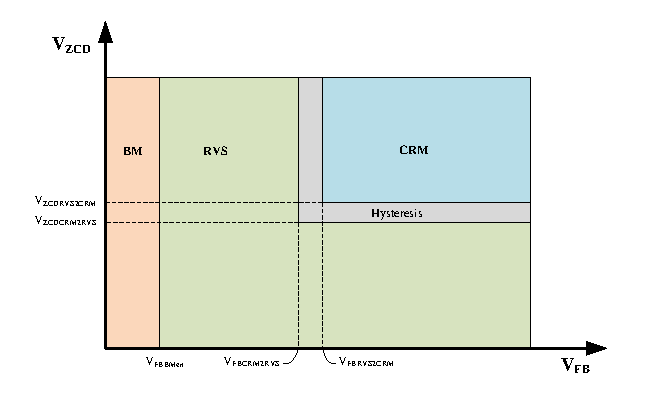
\includegraphics[width=0.6\linewidth]{figures/模式切换1.pdf}
    \caption{多模式切换图}
    \label{fig:模式切换1}
\end{figure}

本文设计了如图~\ref{fig:模式切换1}所示的多模式控制方案,模式切换通过监测引脚FB和引脚ZCD上的电压值来判断输出负载电流和输出电压的大小,一但其超过所设置的不同阈值,模式选择模块控制变换器芯片切换到相应的模式。根据变换器芯片设计,当输出负载电流很小处于极轻载或空载情况时,$V_{FB}$小于对应的参考电压$V_{FBBMen}$,此时芯片被设定为突发工作模式;当输出负载电流逐渐增大进入轻载情况,$V_{FB}$同样随着输出负载电流的增大而增大,且其未大于$V_{FBRVS2CRM}$时,芯片工作在RVS模式中,RVS工作模式是非对称半桥反激式开关电源所特有的一种新型工作模式,能最大化地同时降低高低边功率管的开关损耗;当输出负载电流继续增大,进入重载情况后,$V_{FB}$此时大于$V_{FBRVS2CRM}$,芯片被从RVS工作模式切换为CRM工作模式,在不影响变压器中储能转换的情况下,实现最大的开关频率,最大限度地降低功率管导通损耗并为副边传递能量,维持输出电压在重载下的稳定性。为了防止模式切换时的不稳定性问题,避免芯片在两个模式中来回切换,针对性的设置了CRM模式和RVS模式之间的迟滞区间,当负载电流从重载向轻载切换时,$V_{FB}$则需要小于$V_{FBCRM2RVS}$时,才能由CRM模式切换为RVS模式。由文献可知,AHB反激式变换器系统在轻载时使用CRM模式无法达到最大的能量传递效率,因此输出电压同时制约着不同模式的切换,通过辅助绕组的分压引脚$V_{ZCD}$监测输出电压大小,根据计算和测试,选择输出电压大于15V后才允许芯片从RVS模式切换为CRM模式。为了避免模式之间的频繁切换引起的电路振荡,$V_{ZCD}$同样设置有两个偏置电压$V_{FBRVS2CRM}$和$V_{FBCRM2RVS}$作为迟滞区间。

\begin{figure}[htbp] 
    \centering
    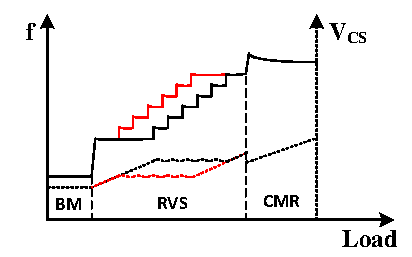
\includegraphics[width=0.6\linewidth]{figures/模式切换2.pdf}
    \caption{多模式频率变化图}
    \label{fig:模式切换2}
\end{figure}

不同的模式影响着功率管的开关频率和峰值电流变化,如图~\ref{fig:模式切换2}所示。

在突发模式时,功率管开关频率和峰值电流都被设定为最小值,通过控制系统间歇性地工作,关断芯片内部除供电模块的所有的控制模块,降低系统的待机功耗;

在RVS工作模式时,功率管开关频率随着输出负载电流的增大呈阶梯式波动,这是由于RVS工作模式为了减小开关损耗,只在高低边功率管中间节点电压$V_{FB}$谐振波谷的谷底处触发导通信号,开始新的周期;为了防止开关频率和峰值电流共同变化导致变换器系统的相位降低引起的稳定性问题,变压器原边电感的峰值电流则不随开关频率的变化产生剧烈波动,通过谷底锁定模块将其维持在一个稳定的区间,以适应输出功率的变化。

在CRM工作模式时,功率管开关频率随着输出负载电流的增大提高到当前变换器系统LC谐振腔允许的最大开关频率;变压器原边电感的峰值电流随输出负载电流的增大而增大,以满足最大工作频率下输出功率的需要。CRM工作模式的工作频率达到最大值后有缓慢减小的趋势,这是由于低边功率管因为LC谐振腔的谐振周期限制了退磁时间的大小,而高边功率管的导通时间随着峰值电流的增大而增大,导致开关周期相应变长,开关频率缓慢降低。

\subsection{CRM工作模式}

\subsection{RVS工作模式}

\begin{figure}[htbp] 
    \centering
    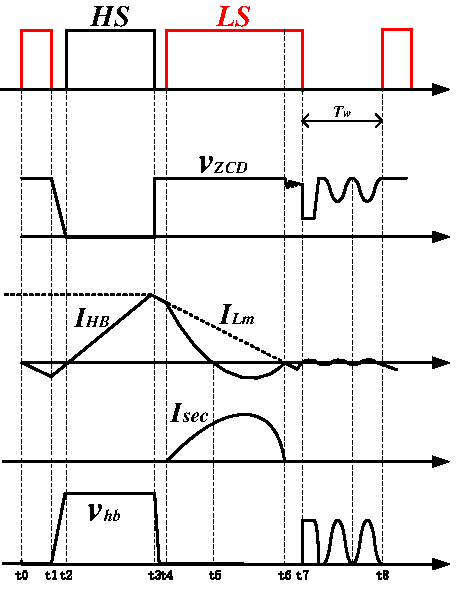
\includegraphics[width=0.6\linewidth]{figures/RVS波形图.pdf}
    \caption{RVS工作模式波形图}
    \label{fig:RVS波形图}
\end{figure}

RVS工作模式是针对非对称半桥反激式开关电源设计的一种新型的DCM操作模式,旨在轻载工况下消除高低边功率管的输出损耗。由于非对称半桥反激式变换器拓扑结构初级测和LLC型开关电源相同,存在谐振电容Cr和变压器漏感Lr组成的谐振腔,因此当控制器处于DCM控制模式时,高低边功率管都关闭的等待时间内产生谐振现象,如图~\ref{fig:RVS波形图}中Tw时间。因此无法在等待时间内利用逆向电感电流将高低边功率管中间节点电压$V_{HB}$充电到等于输入电压$V_{in}$,高边功率管存在较大的源漏电压差$V_{DS}(V_{DS}=V_{in}-V_{HB})$,故在非对称半桥反激式系统中使用传统的DCM控制方式导通高边功率管会产生巨大的开关损耗,降低电路的能量传递效率,因此非对称半桥反激式系统中一般使用边界导通(BCM)模式,BCM工作模式在重载时具有最佳的效率,在轻载时同样存在一定的问题,如能量传递延后和能量传递出现双脉冲等情况。根据文献的研究,提出了新型的谐振谷值开关工作(RVS)模式。

此控制方式巧妙地在开启高边功率管前,提前打开底边功率管一定时间,产生逆向的电感电流为$V_{HB}$节点进行充电,合理规划死区时间即可将$V_{HB}$节点电压充电到等于$V_{in}$,此时再打开高边功率管对变压器原边电感进行励磁储能,极大的降低开关损耗和能量传递效率,具体波形图如图~\ref{fig:RVS波形图}所示。同时考虑到等待时间内$V_{HB}$的谐振情况,通过精确谷底导通模块控制低边功率管在$V_{HB}$电压谐振谷底处导通,抑制低边功率管引入的不必要的开关损耗。



\section{关键技术}
\subsection{精确谷底导通技术}
在RVS控制模式时,一个周期内存在高低边功率管都关断的等待时间阶段,此时原边电感不给副边传递能量,电感电压出现谐振现象。为了满足RVS控制模式的低开关损耗,设计精确谷底导通电路实现$V_{HB}$电压谐振谷底处导通低边功率管,减小低边功率管的开关损耗。

电路存在两个困难点,一方面是需要测量$V_{HB}$谐振电压谷底,产生对应谷底信号参与后续逻辑控制;另一方面是由于驱动电路存在的信号延时问题,会导致实际控制功率管的开关信号比PMW信号更晚产生,以致于实际低边功率管不在$V_{HB}$谐振谷底处导通,产生不必要的开关损耗。

图 是RVS模式中一个周期内$V_{HB}$信号的波形图,在等待时间内,由于原边漏感Lr和原边谐振电容Cr产生电感电容谐振;但因为$V_{HB}$电压过高无法接入芯片内进行采样处理,因此将原边电感电压通过电阻分压后产生$V_{ZCD}$信号传入变换器内采样。图 是$V_{ZCD}$电压信号的波形图,$V_{ZCD}$信号和$V_{HB}$信号谐振相反,$V_{HB}$的谐振谷底对应$V_{ZCD}$的谐振峰值。使用峰值检测电路来检测$V_{ZCD}$信号在等待时间内的谐振峰值,图 是峰值检测电路的电路图。再通过比较器产生峰值脉冲信号用于后续逻辑控制。

因为存在驱动器等电路的延时,为了实现精确的谷底导通功能,通过需要在$V_{HB}$谐振谷底到来之前产生低边功率管的导通逻辑信号,使得逻辑信号通过驱动器后,产生的实际控制低边功率管导通信号刚好处于$V_{HB}$信号谐振谷底的位置处,因此要求逻辑信号提前产生的时间等于驱动器等电路的延时时间。图~\ref{fig:精确谷底导通电路图1}是精确谷底导通信号的电路图。

\begin{figure}[htbp] 
    \centering
    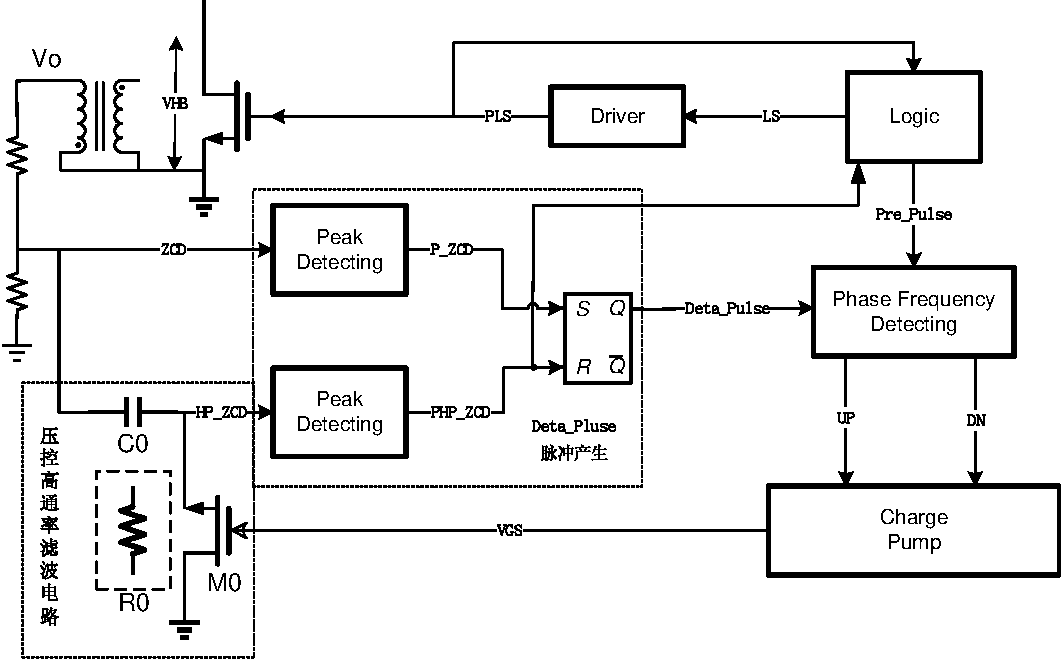
\includegraphics[width=0.8\linewidth]{figures/精确谷底导通电路图1.pdf}
    \caption{精确谷底导通电路图}
    \label{fig:精确谷底导通电路图1}
\end{figure}

LS和PLS分别是PWM控制电路产生的低边功率管控制信号和实际控制信号,通过逻辑控制电路得到LS和PLS信号的延时时间Pre\_Pulse。为了预判谷底信号,通过一个使用MOS管充当电阻的压控高通滤波器电路,产生$V_{ZCD}$对应的超前时间信号VHP\_ZCD,只需适当的调节VGS的大小即可控制VHP\_ZCD信号的超前时间大小。分别使用两个峰值检测电路来检测并得到两个信号的峰值脉冲信号,经过SR锁存器产生超前时间Deta\_Pulse。为了轻微的调节栅极电压信号VGS,使用了PLL电路中的鉴相鉴频器和电荷泵电路来控制Deta\_Pulse信号逐步逼近Pre\_Pulse信号,完成低边功率管的精确谷底导通功能。

\subsection{退磁时间动态校准技术}

非对称半桥反激式变换器系统通过导通高边功率管对变压器原边励磁电感和谐振电容进行储能,导通低边功率管对励磁电感和LC谐振腔中的能量传递到变压器副边的输出电容中,高低边功率管的交替导通实现在不同负载情况下系统的宽范围输出电压稳定。不同于高边功率管的导通时间由峰值电流决定,低边功率管的导通时间设置目前仍未得到广泛探索,低边功率管导通时间过长或过短都存在一定的问题。

过长的低边功率管导通时间实现了变压器副边二极管的ZCS关断,但在高输出电压的情况下会增大不必要的导通损耗,且会继续LC谐振腔内的能量,影响下一周期副边二极管的正向偏置,产生可靠性问题;过短的低边功率管导通时间既可能造成副边的电流纹波增大,无法实现副边二极管ZCS关断,又未能将励磁能量完全传递到副边输出电容,影响系统传递效率。因此无论是重载工况下的CRM工作模式还是轻载工况时的RVS工作模式,都要求低边功率管的最佳导通时间是导通后在励磁电感退磁完成时刻关断功率管。

由文献可知,如~\ref{fig:RVS波形图}中的t6时刻,当变压器原边电感电流$I_{Lm}$和$I_{Lr}$相等时,变压器副边电流$I_{sec}$同时降低为0,原边励磁电感退磁完成,此时副边二极管的寄生电容$C_{pj}$迅速放电且与变压器漏感发生高频谐振,谐振频率公式如\eqref{eq:ZCD谐振公式}所示。

\begin{equation}
    \label{eq:ZCD谐振公式}
    f_{hp} = \frac{1}{2\pi \sqrt{L_r * C_{pj}/N^2}}
\end{equation}

其中 
\begin{equation}
    \label{eq:变压器匝比}
    N=\frac{N_P}{N_S}
\end{equation}

此高频谐振现象可以在ZCD引脚中观察到,故通过对ZCD引脚电压$V_{ZCD}$进行采样处理后,即可得到励磁电感退磁完成信号LST\_e。

包含有退磁时间动态自校准模块的非对称半桥反激式变换器系统的简单框图如图~\ref{fig:退磁时间1}所示,辅助绕组$N_A$上的绕组电压由电阻$R_1$和$R_2$分压后通过ZCD引脚输入变换器芯片中,经采样保持电路处理后输入给退磁时间动态校准模块,最终该模块输出低边功率管的导通时间信号$T_{Q2}$。在模块中不仅需要检测出上文所提到的ZCD引脚上的高频谐振现象,同时输出负载电流波动还会导致的励磁电感退磁完成时刻不固定的问题,针对此问题该模块还新颖的设计了动态自校准的方案,避免低边功率管导通时间随着退磁完成时刻的波动而剧烈变化,引入不必要的人为电路噪声和不稳定性问题,通过一系列电路设计,使得低边功率管导通时间在退磁完成时刻波动后,随着周期的推进,导通时间动态地逐步逼近到退磁完成时刻,实现对退磁完成时刻的精确校准,既满足副边电流ZCS的关断又达到励磁电感能量最佳传递效率。

\begin{figure}[htbp] 
    \centering
    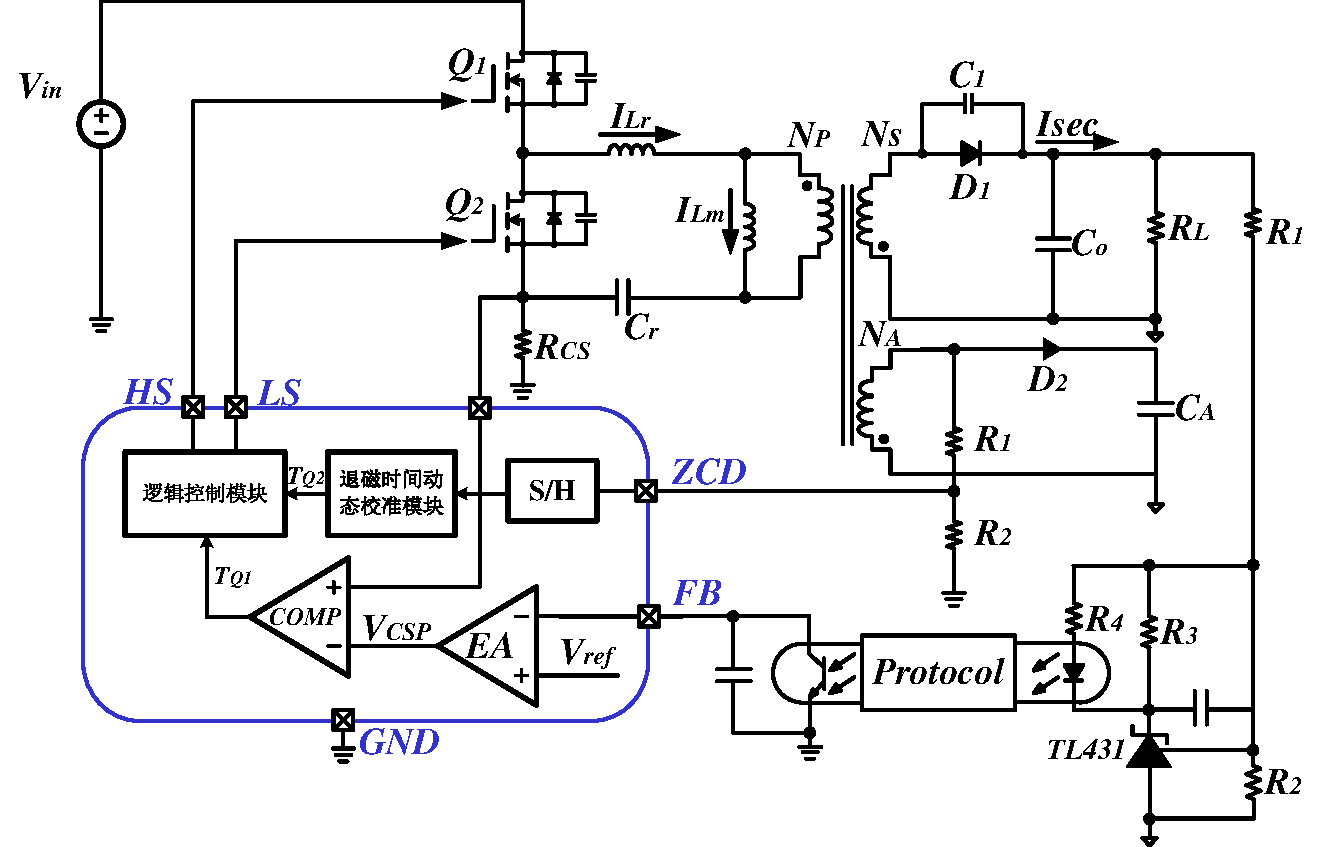
\includegraphics[width=0.8\linewidth]{figures/退磁时间动态校准图.pdf}
    \caption{退磁时间动态校准技术框图}
    \label{fig:退磁时间1}
\end{figure}














\section{小结}





\chapter{电路设计与仿真}

本章对基于Cadence Virtuoso仿真软件和SMIC 0.18um BCD工艺设计的变换器芯片的各个关键电路进行分析和仿真,包括欠压锁定电路、内部供电电路、模式切换电路、退磁时间动态校准电路、峰值电流控制电路、精确谷底导通电路、谷值锁定电路、逻辑控制电路和各个保护电路等。最后对整体电路进行系统仿真,测试变换器芯片的基本功能,验证该电路设计的合理性和可靠性。

\section{欠压锁定电路}

\subsection{欠压锁定电路工作原理}

在高压稳压电路中,还包含了欠压锁定电路(Under Voltage Lockout On VDD, UVLO),即当外部输入电源电压低于预设值时,作为负载的逻辑电路可能会产生误操作,从而导致系统进入异常工作状态。因此我们需要在系统中设计欠压锁定电路。

当外部输入电源电压低于预设值时,UVLO电路会输出高电平,直接控制外置功率开关管关断,同时内部低压电源供电电压均输出低电平;当外部电源电压高于预设值(即正常输入)时,UVLO输出低电平, 内部低压供电电源电压正常输出5V电压,表示芯片上电启动完成。电路原理图如图~\ref{fig:UVLO电路}所示。

\begin{figure}[htbp] 
    \centering
    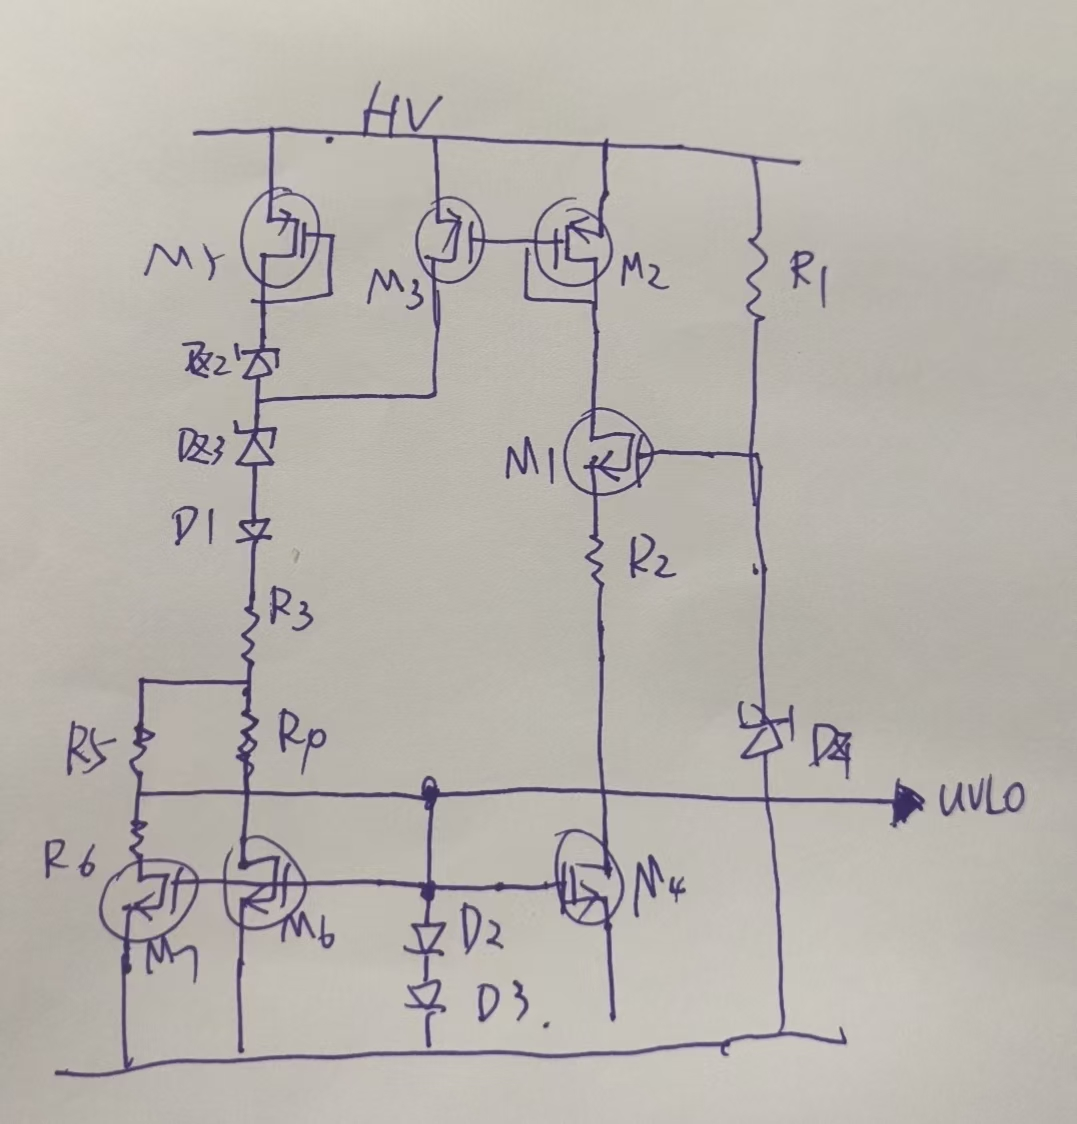
\includegraphics[width=0.6\linewidth]{figures/UVLO电路.jpg}
    \caption{欠压锁定UVLO电路原理图}
    \label{fig:UVLO电路}
\end{figure}

欠压锁定电路的工作原理是通过高压LDMOS和齐纳二极管对输入电压进行箝位,当输入电压逐渐升高到大于齐纳二极管$D_{Z1}$时,节点电压V1被箝位至二极管$D_{Z1}$的反向击穿电压$V_{DZ1}$,V1作为高压管MN1的栅极电压同时将其导通。MN1导通后由于MN2未导通故无电流产生,其源端电压等于UVLO,此时UVLO电压较大,可视为逻辑“1”。MN3和MN4同时被栅极电压UVLO导通,将MN3和MN4的漏端同时拉到地电位,电阻R4并联于R5和R6的串联。
随着输入电压继续增大,节点电压V5由于自偏置高压管MP3产生的电流持续流过电阻R3,节点电压V6、V5和V4也随着输入电压持续增大。其中V6电压的公式为:
\begin{equation}
    %\label{eq:Vbe公式}
    V_6 = V_{IN} - V_{GS,MP3} - V_{DZ2} - V_{DZ3} - V_{D4}  
\end{equation}
直至节点电压V4增大至大于晶体管MN2的阈值电压$V_{TH,MN2}$时,晶体管MN2导通,将输出电压UVLO直接拉低到地电位,表明此刻输入电压脱离欠压锁定状态。此时的输入电压等于脱离欠压锁定的电压$V_{UVLO,OFF}$的电压值,电压$V_{UVLO,OFF}$的公式可表达为:
\begin{equation}
    \label{eq:V_UVLO,OFF公式}
    V_{UVLO,OFF} = V_5 + I_{R3}R_3 + V_{GS,MP3} + V_{DZ2} + V_{DZ3} + V_{D4}  
\end{equation}
其中R3上流过的电流$I_{R3}$的公式可表示为:
\begin{equation}
    \label{eq:IR3公式}
    I_{R3} = I_{R4} + I_{R5} = \frac{V_5 - V_{DS,MN3}}{R_4} +  \frac{V_5 - V_{GS,MN2}}{R_5}
\end{equation}

当输入电压从高压逐渐降低到一定值时,同样会进入欠压锁定情况中。在未进入欠压锁定状态时,由于MN4在输出UVLO为低电平时被关断,此时节点电压V4和V5相等。
随着输入电压逐渐降低,节点电压V4和V5的电压值也跟随着降低,直至当输入电压低于齐纳二极管的的反向击穿电压时,V5也低于晶体管MN2的阈值电压$V_{TH,MN2}$时,晶体管MN2关断,其漏端电压UVLO重新被瞬间拉高,电路再次进入欠压锁定转态。

\subsection{欠压锁定电路仿真分析}

\begin{figure}[htbp] 
    \centering
    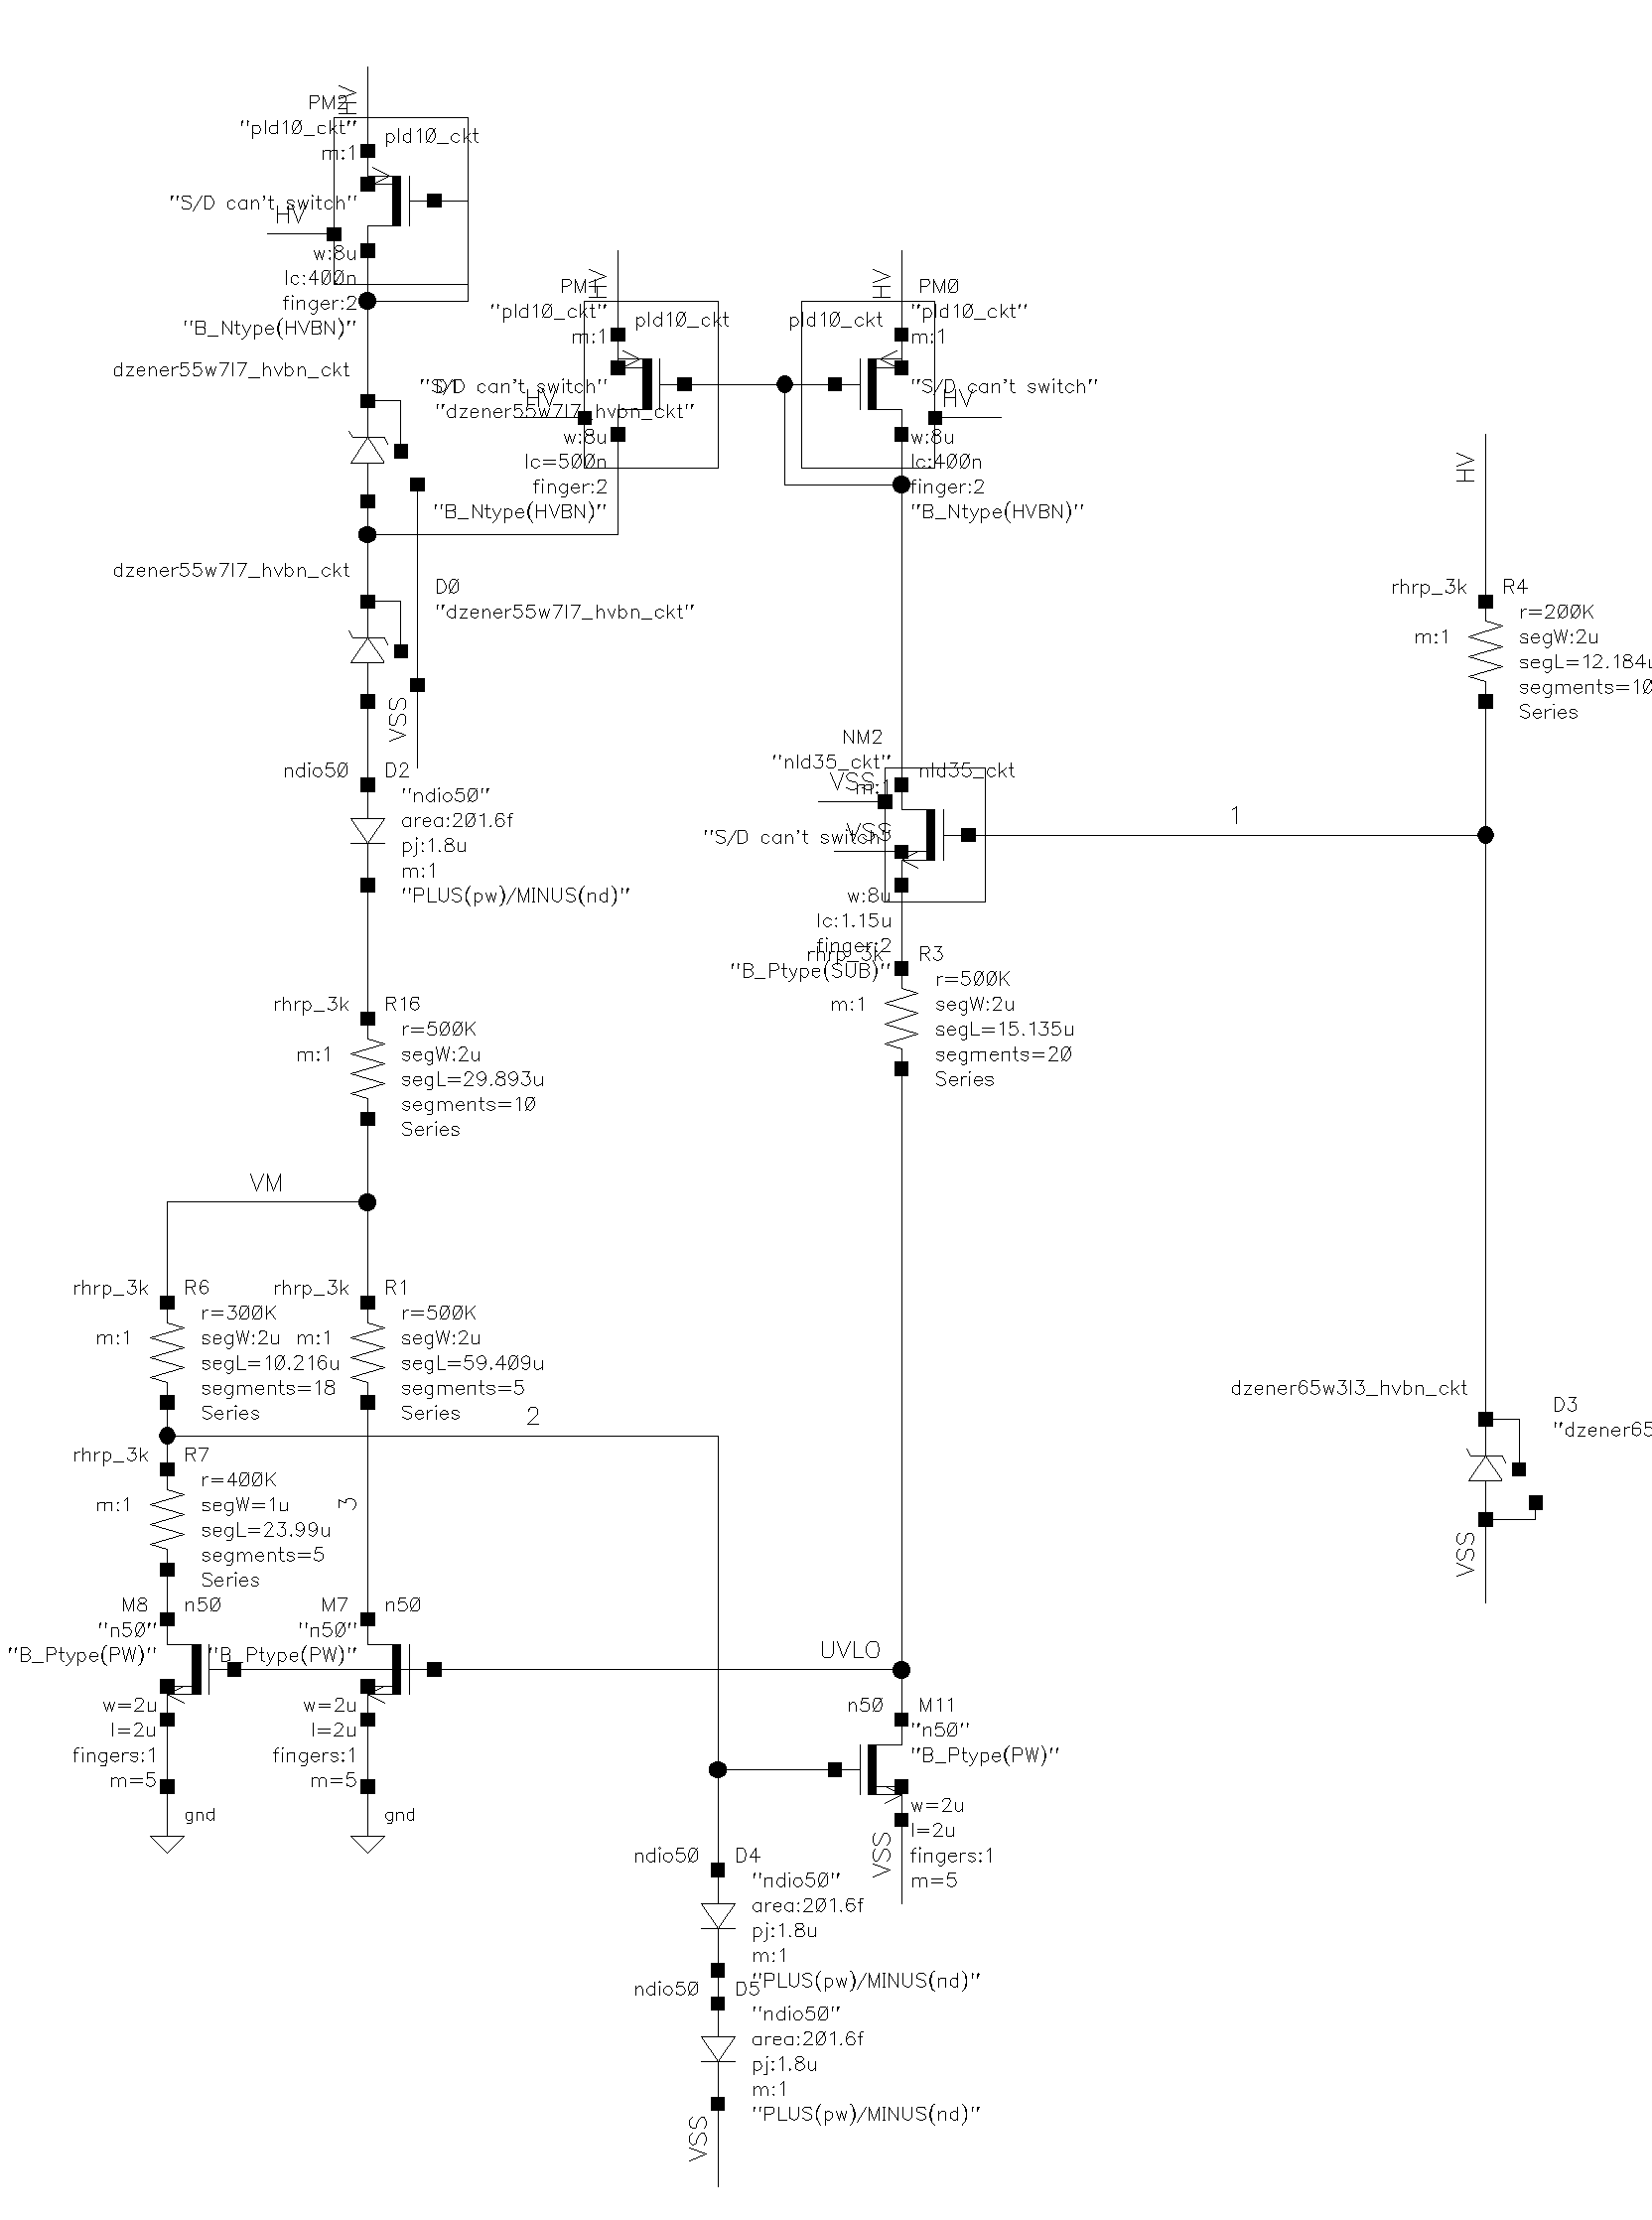
\includegraphics[width=0.8\linewidth]{figures/UVLO.png}
    \caption{欠压锁定UVLO电路仿真图}
    \label{fig:UVLO电路仿真}
\end{figure}

欠压锁定电路的仿真结果如图~\ref{fig:UVLO电路仿真}所示。
仿真结果表明,该欠压锁定电路正常完成其功能,性能符合变换器芯片要求。测试所用的输入电压HV输入范围为0-20V,当输入电压从低压逐渐升高至14.3V前,欠压锁定电路的输出电压UVLO电压为高电平,表明此时电路处于欠压锁定状态,芯片内部模块都未开始工作;当输入电压大于14.3V后,输出电压UVLO翻转为低电平,片内各模块进入正常工作转态。当输入电压从高压逐渐降低至6.5V时,欠压锁定电路输出电压UVLO重新被提升至高电平,电路重新进入欠压锁定状态,片内所有电路重新停止工作。




\section{内部供电电路}

\subsection{带隙基准电路}

在变换器芯片工作过程中,其内部的各个模块都需要相应的偏置电压和偏置电流,为了维持这些偏置电压和偏置电流的精确和稳定性,不能用普通的与电源无关的基准电路产生全部的信号,因此需要设计带隙基准电路,提供受电源电压和温度变化影响很小的基准电压电流,使得变换器芯片适用于各种工况下。

带隙基准电路的实现原理是通过将一个正温度系数的电压和一个负温度系数的电压加权相加后,抵消掉其正负温度系数,得到不受温度变化影响的零温度系数的基准电压。实际电路中,负温度系数的电压利用双极型晶体管产生,其正向压降$V_{be}$带有负温度特性。通过半导体物理的基础知识可知,电压$V_{be}$的公式为:
\begin{equation}
    \label{eq:Vbe公式}
    V_{be} = V_T \cdot ln(\frac{I_c}{I_s})
\end{equation}
其中,$V_T$是热电压,公式为:
\begin{equation}
    \label{eq:VT公式}
    V_T=\frac{kT}{q}
\end{equation}
$I_c$是PN结的集电极电流,公式为:
\begin{equation}
    \label{eq:Ic公式}
    I_c=I_s \cdot exp(\frac{V_{be}}{V_T})
\end{equation}
$I_s$是PN结饱和电流,公式为:
\begin{equation}
    \label{eq:Is公式}
    I_s=bT^{4+m} exp\frac{-E_g}{kT}
\end{equation}
结合式\eqref{eq:Vbe公式}、\eqref{eq:Ic公式}和\eqref{eq:Is公式},通过正向压降$V_{be}$对温度求偏导,可计算得$V_{be}$的负温度系数公式:
\begin{equation}
    \label{eq:Vbe/T公式}
    \frac{\partial V_{be}}{\partial T} = \frac{ V_{be} - (4+m)V_T - E_g/q}{T}
\end{equation}

正温度系数的电压同样可以通过双极型晶体管来产生,不同电流密度的电流流经晶体管会产生不同的负温度系数,两者的差值电压$\varDelta V_{be}$带有正温度系数。实际电路中为了满足晶体管的匹配性,使用两个不同面积的双极型晶体管来产生不同电流密度的作用。令两个双极型晶体管的面积比为$1:N$,则流经单个晶体管的电流密度比N:1,可计算得晶体管压差$\varDelta V_{be}$的公式为:
\begin{equation}
    \label{eq:△Vbe公式}
    \varDelta V_{be} = V_T ln(\frac{I_c}{I_s}) - V_T ln(\frac{I_c}{nI_s}) = V_T \cdot ln(n)
\end{equation}
通过$\varDelta V_{be}$对温度求偏导可计算得正的温度系数公式:
\begin{equation}
    \label{eq:△Vbe/T公式}
    \frac{\partial \varDelta V_{be}}{\partial T} = \frac{k}{q}\cdot ln(n)
\end{equation}


由式\eqref{eq:Vbe/T公式}和\eqref{eq:△Vbe/T公式}计算可知,在常温T=300K的条件下,当$V_{be}\thickapprox $ 750 mV时,$V_{be}$的负温度系数约等于-1.5 mV/K,$\varDelta V_{be}$的正温度系数为0.087ln(n) mV/K。为了合理地产生零温度系数电压,防止双极型晶体管的面积太大,需对正负温度系数加权相加可得。

为了满足变换器芯片中的低压数字模块,



\subsection{高压LDO电路}

由辅助绕组产生的供电端电压对于片内的元器件而已电压过大且不够稳定,无法直接用于作为供电电压,需要设计用于产生稳定输出电压的低压线性稳压器电路,将供电端的高压转化为可为内部电路供电的电源电压输出。
\begin{figure}[htbp] 
    \centering
    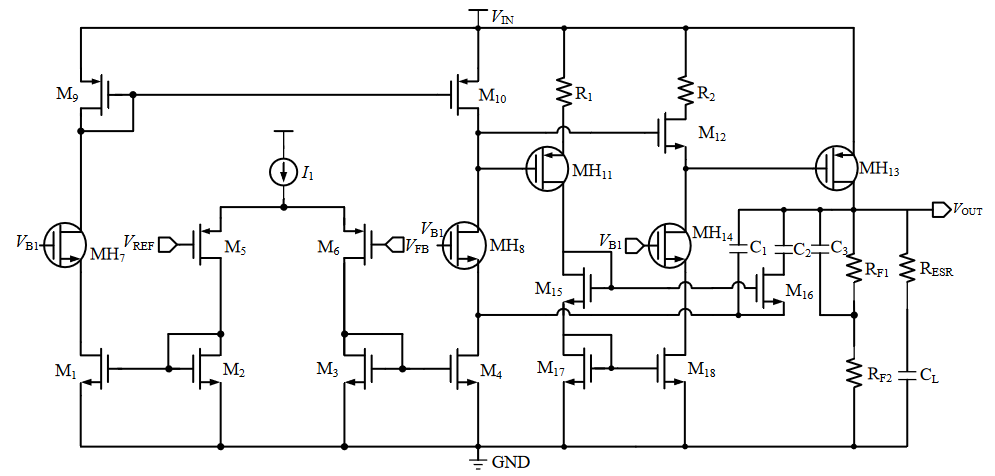
\includegraphics[width=0.6\linewidth]{figures/高压LDO.png}
    \caption{高压LDO电路图}
    \label{fig:高压LDO}
\end{figure}

本文设计的高压LDO电路如图~\ref{fig:高压LDO}所示,该电路


%\section{抖频振荡器}

%\section{模式切换电路}



\section{宽输出电压补偿的峰值电流控制电路}
\label{sec:峰值电流控制电路}
\subsection{宽输出电压补偿的峰值电流控制电路工作原理}

在宽输出范围非对称半桥反激式变换器系统中,随着输出电压的提升,相同负载下输出功率也随之提高,低输出电压下的高边功率管导通时间HSGD内存储在励磁电感和谐振腔内的能量已无法满足高输出电压下输出功率的要求,系统将自动提高峰值电流电压以产生更长的导通时间HSGD存储更多的能量传递到副边,进而要求更大的副边反馈电压$V_{FB}$,影响电路内各种模块的正常功能,产生各种不稳定的情况。

副边反馈电压$V_{FB}$随输出电压的波动是因为其是峰值电流电压$V_{CSP}$的重要组成部分,为了满足变大的输出功率,在开关频率不变的情况下,高边功率管更长的导通时间对应着更大的峰值电流$V_{CSP}$,$V_{FB}$也相应地增大。
故为满足变换器系统的宽输出范围的工作需求,设计了宽输出电压补偿结构的峰值电流控制电路来根据输出电压对峰值电流电压$V_{CSP}$进行补偿,维持副边反馈信号在宽输出范围内均匀地分布在全负载下。

%根据上文~\ref{sec:电流控制模式}小节的分析,如图~\ref{fig:电流工作模式电路图}中所示,可知副边反馈引脚电压信号是峰值电流电压$V_{CSP}$的重要组成部分,其可以一定程度地反映输出负载电流的大小。当负载电流突然增大时,为了满足变大的输出功率,变压器原边需要增加高边功率管的导通时间提供更多的能量传递给输出电容,因此$V_{CSP}$增大,$V_{FB}$也相应地增大;当负载电流突然减小时,同理$V_{FB}$也相应地减小。但在不同输出电压的情况下,相同负载电流下,信号$V_{FB}$稳定后电压值却大不相同,严重影响了芯片内多种电路模块,如精确谷底导通、谷值锁定、退磁时间动态校准等模块对$V_{FB}$的采样要求。为了避免此问题,需要设计峰值电流控制电路实现在当输出电压不同时,仍能维持信号$V_{FB}$的电压值在负载电流不变情况下的一致性。

在峰值电流控制模式中,峰值电流电压$V_{CSP}$是通过采样电阻对电感电流采样实现的,具体的转换关系可表示为:
\begin{align}
    \label{eq:VCSP公式}
    V_{CSP} = I_P \cdot R_{CS} 
\end{align}
其中$I_P$为原边电感电流的峰值。

\begin{figure}[htbp] 
    \centering
    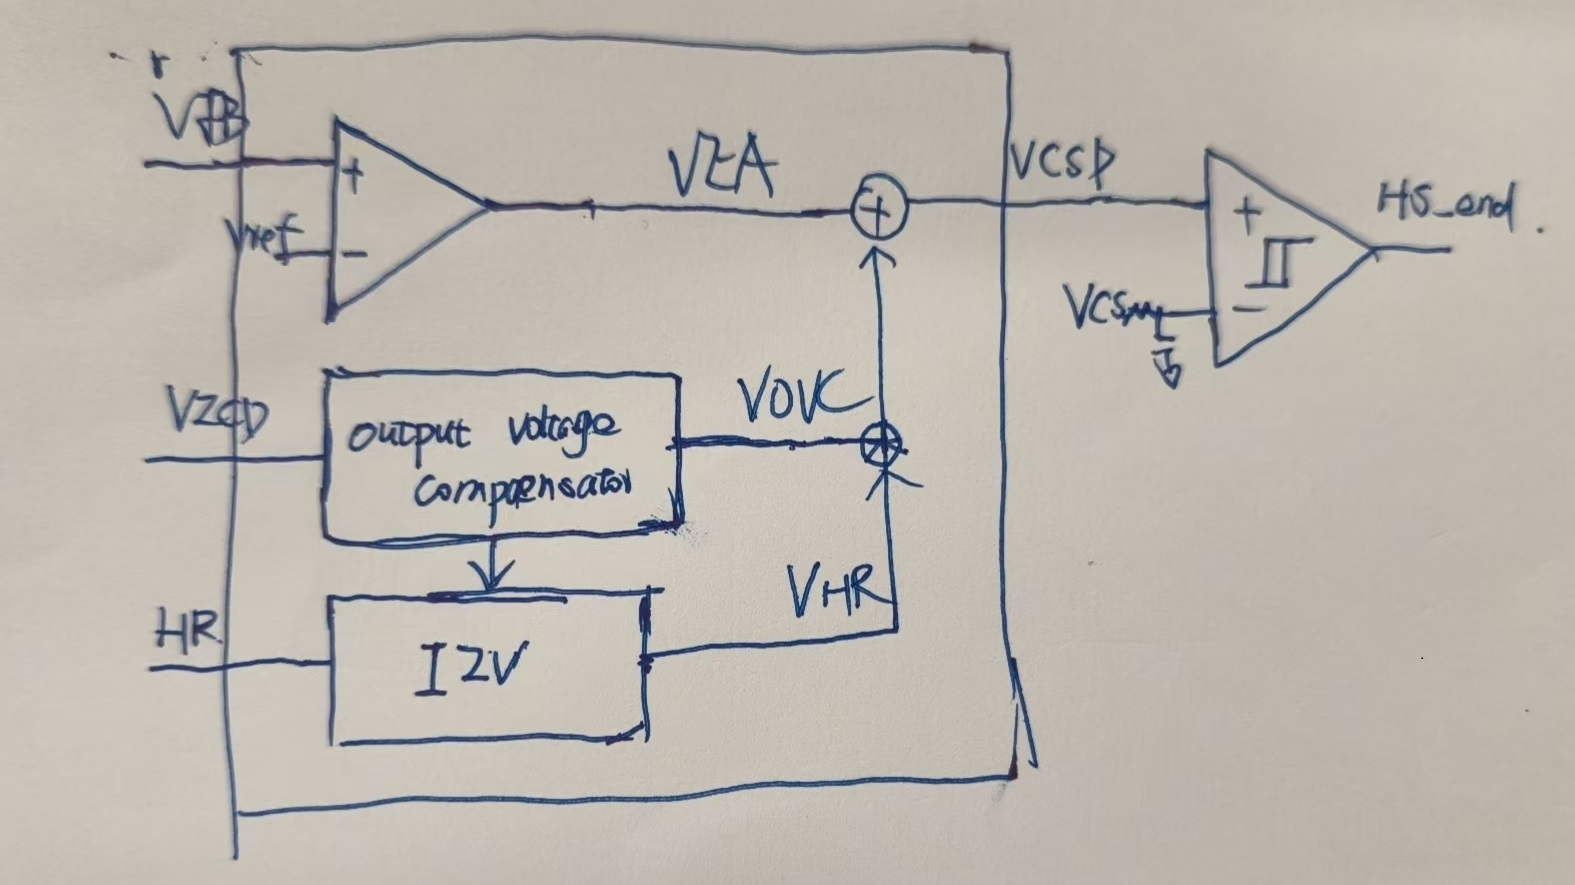
\includegraphics[width=0.8\linewidth]{figures/峰值电流控制.jpg}
    \caption{峰值电流控制电路框图}
    \label{fig:峰值电流控制框图}
\end{figure}

由于需要考虑到不同输出电压的影响,因此峰值电流电压$V_{CSP}$不能完全由副边反馈电压$V_{FB}$计算产生,需要引入携带输出电压信息的$V_{ZCD}$信号对$V_{CSP}$进行补偿,实现高边功率管导通时间在$V_{FB}$维持不变的情况下随着输出电压的变化而自动变化。其中辅助绕组电压$V_{ZCD}$和输出电压的关系如式\eqref{eq:VZCD公式}所示。

片内峰值电流电压$V_{CSP}$产生电路的框图如图~\ref{fig:峰值电流控制框图}所示,峰值电流电压$V_{CSP}$由电压信号$V_{EA}$、$V_{OVC}$和$V_{HR}$加权求和所得。电压$V_{EA}$是信号$V_{FB}$乘以反馈电压衰减系数$k_1$所得;$V_{OVC}$是输出电压补偿信号,由输出电压$V_o$乘以输出电压补偿结构衰减系数$k_2$所得;$V_{HR}$是切换为RVS工作模式时的补偿电压,用来补偿模式切换时开关频率骤变后的峰值电流变化。$V_{CSP}$的公式可表达为:
\begin{align}
    \label{eq:VCSP公式1}
    V_{CSP} &= V_{EA} + V_{OVC} + V_{HR} \\ &= k_1 V_{FB} + k_2 V_o + V_{HR}  
\end{align}
通过合理设置系数$k_1$和$k_2$的值,当输出电压切换导致$V_{CSP}$波动时,可以维持$V_{FB}$的稳定。

下面分析峰值电流电压和高边功率管导通时间在CRM工作模式中不同输出电压下的关系。图~\ref{fig:峰值电流控制1}中显示了在不同输出电压下峰值电流电压、电感电流斜率和占空比的关系。当输出电压为$V_{o1}$时,对应的峰值电流电压为$V_{CSP1}$,高边功率管导通时间HSGD为$D_1T_s$;当输出电压为$V_{o1}$时,对应的峰值电流电压为$V_{CSP2}$,高边功率管导通时间HSGD为$D_2T_s$。其中,根据式\eqref{eq:CCM_4}可求得$\frac{D2}{D1} = 4$。但由于电感电流的斜率也会发生变化,不能直接将占空比的变化值直接套用于计算$V_{CSP2}$和$V_{CSP1}$的比值。结合式\eqref{eq:Vcr_1}电感电流的斜率$K_{slope}$的公式可表示为:
\begin{equation}
    \label{eq:电感电流斜率公式}
    K_{slope} = \frac{V_{in} - N V_o}{L_m}
\end{equation}
由式\eqref{eq:电感电流斜率公式}可见,电感电流斜率会随着输出电压的变化而变化,输出电压越大,斜率越小。因此,在输出电压变化的情况下,峰值电流电压$V_{CSP}$的变化和占空比D的变化不成正比,不能直接对$V_{CSP}$乘以输出电压变化的倍数计算变化后的$V_{CSP}$。

\begin{figure}[htbp] 
    \centering
    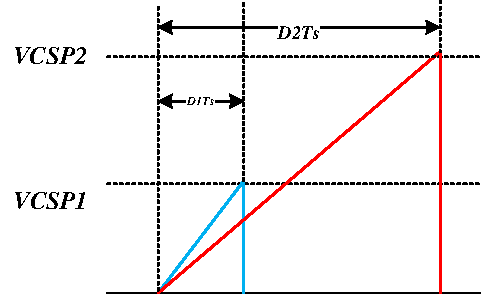
\includegraphics[width=0.6\linewidth]{figures/峰值电流控制1.pdf}
    \caption{不同输出电压下的峰值电流电压波形}
    \label{fig:峰值电流控制1}
\end{figure}

结合图~\ref{fig:峰值电流控制1}中带入公式\eqref{eq:电感电流斜率公式}得峰值电流电压的公式为:
\begin{equation}
    \label{eq:VCSP公式2}
     V_{CSP} = K_{slope} \cdot DT_s = \frac{V_{in} - N V_o}{L_m} \cdot \frac{N V_o}{V_{in}} T_s
\end{equation}

分别将两个不同的输出电压$V_{o1}$和$V_{o2}$带入式中,可计算得$V_{CSP1}$和$V_{CSP2}$的比值为:
\begin{equation}
    \label{eq:VCSP公式3}
    \frac{V_{CSP2}}{V_{CSP1}} = \frac{4 (V_{in} - NV_{o1})}{V_{in} - NV_{o2}}
\end{equation}
故当测得单一输出电压下的峰值电流电压值后,其他输出电压下的$V_{CSP}$也都可计算求出。

为计算输出电压补偿衰减系数$k_2$的值,将不同的输出电压带入式\eqref{eq:VCSP公式1}中并作差可得:
\begin{equation}
    \label{eq:VCSP公式4}
    \varDelta V_{CSP} = V_{CSP2}-V_{CSP1} = k_2 (V_{o2} - V_{o1})
\end{equation}

将式\eqref{eq:VCSP公式3}带入式\eqref{eq:VCSP公式4}中可求得输出电压补偿衰减系数$k_2$的公式为:
\begin{equation}
    \label{eq:k2公式}
    k_2 = \{ \frac{4 (V_{in} - NV_{o1})}{V_{in} - NV_{o2}} - 1 \} V_{CSP1} \cdot \frac{1}{V_{o2} - V_{o1}}
\end{equation}

\begin{figure}[htbp] 
    \centering
    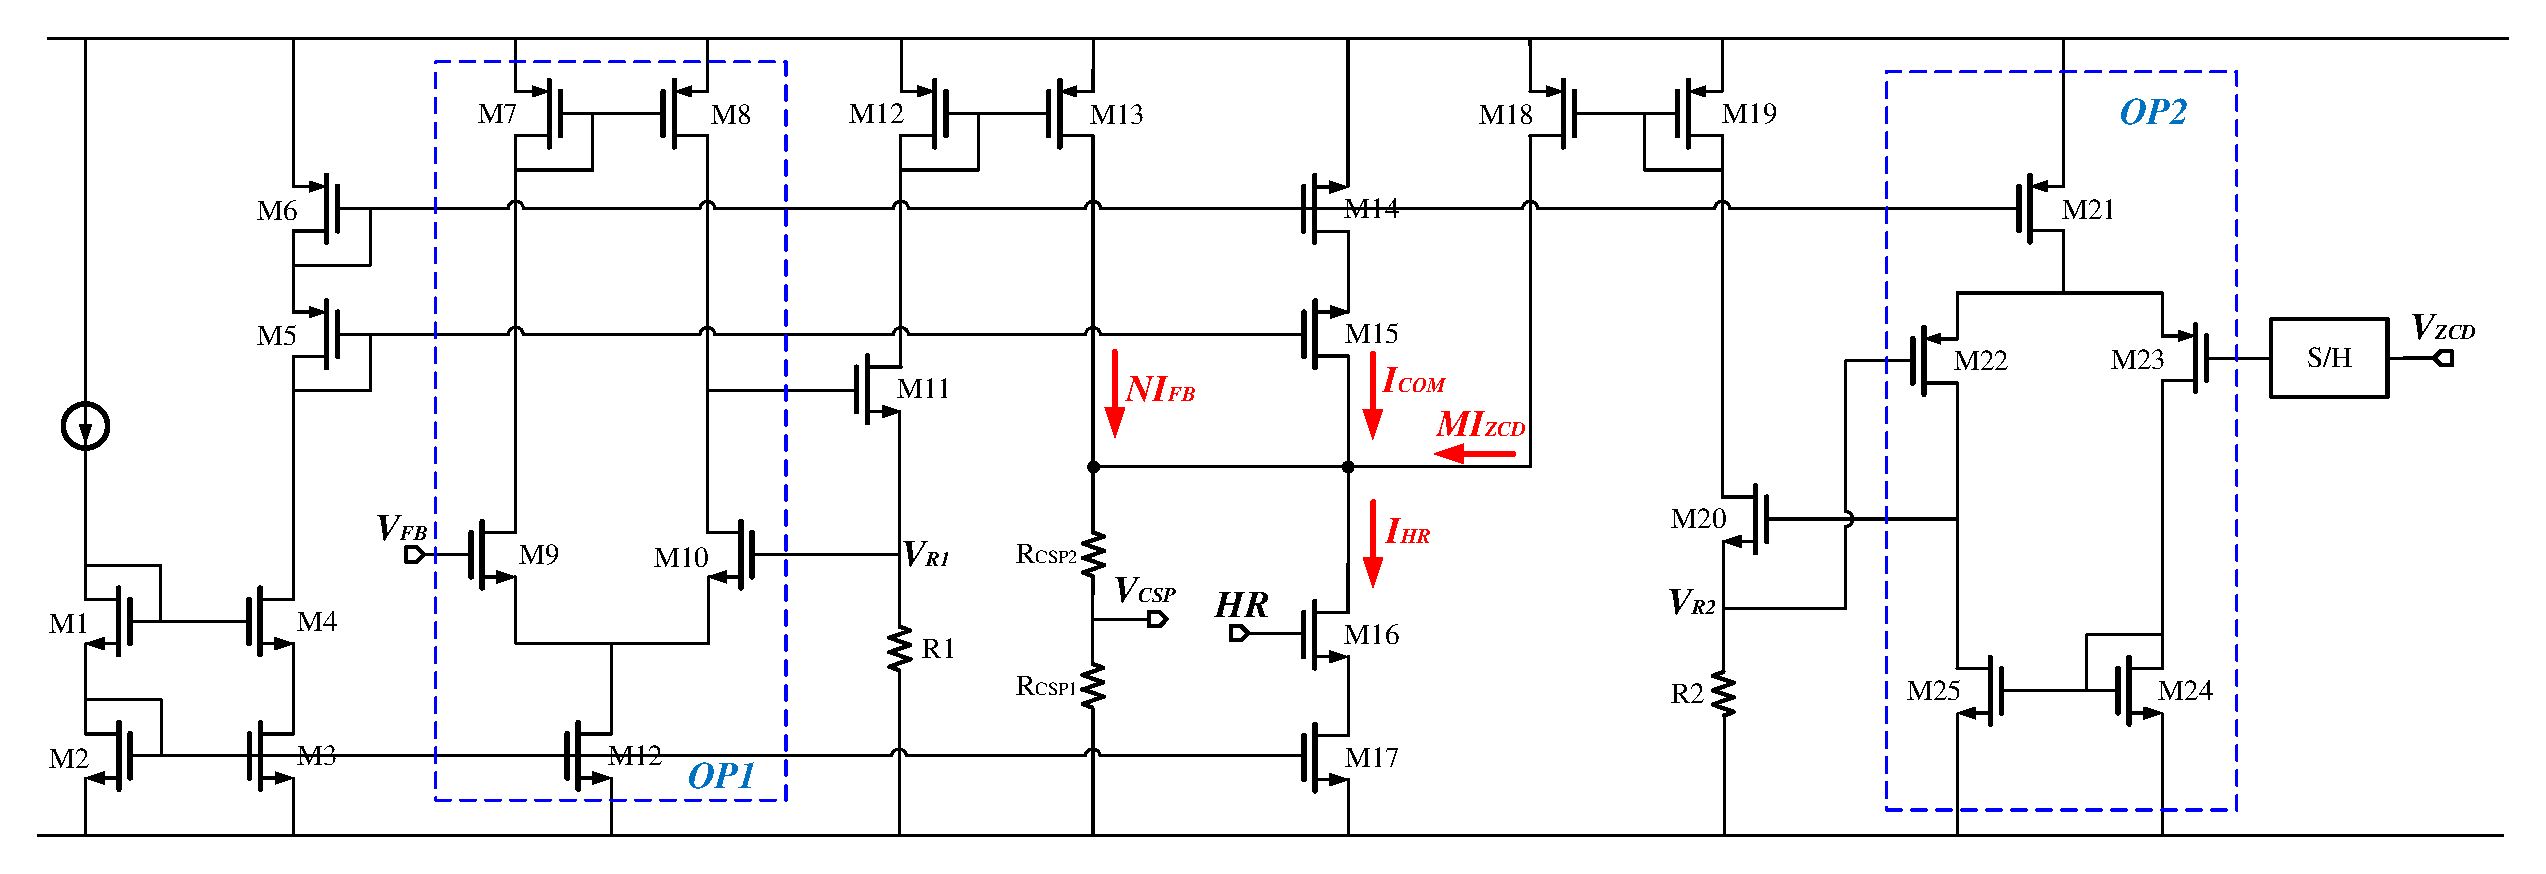
\includegraphics[width=1.0\linewidth]{figures/峰值控制电路图.pdf}
    \caption{峰值控制电路电路图}
    \label{fig:峰值控制电路图}
\end{figure}

带有宽输出电压补偿结构的峰值电流控制电路的具体电路图如图~\ref{fig:峰值控制电路图}所示。图中包括两个运放OP1和OP2组成的VCCS结构,该电路通过运放的虚短作用将OP1的输入端$V_{FB}$箝位到$V_{R1}$,$V_{R1}=V_{FB}$,调节运放输出端的电压控制晶体管M11的漏电流等于$I_{FB}$,同理运放OP2也将$V_{ZCD}$通过采样保持模块后产生的电压$V_{ZCD,in}$转化为电流$I_{ZCD}$。其中$I_{FB}$和$I_{ZCD}$的公式表达为:
\begin{equation}
    \label{eq:IFB公式}
    I_{FB} = \frac{V_{FB}}{R_1}
\end{equation}
\begin{equation}
    \label{eq:IZCD公式}
    V_{CSP} = \frac{V_{ZCD,in}}{R_2}
\end{equation}
电流信号$I_{FB}$通过电流镜M12、M13镜像为电流$NI_{FB}$后,该电流流过电阻$R_{CSP1}$,形成电压$V_{EA}$,其中$V_{EA}=k_1V_{FB}$;电流信号$I_{ZCD}$通过电流镜M18、M19镜像为电流$MI_{ZCD}$后,该电流同样流过电阻$R_{CSP1}$,形成电压$V_{OVC}$,$V_{OVC}$的公式可表示为:
\begin{equation}
    \label{eq:VOVC公式}
    V_{OVC} = \frac{MR_{CSP1}}{R_2}  V_{ZCD,in}
\end{equation}
除此之外,$R_{CSP1}$上的电流还包括补偿电流信号$I_{com}$和用于补偿模式切换的电流信号$I_{HR}$,分别在$R_{CSP1}$上形成电压$V_{com}$和$V_{HR}$。电压$V_{com}$用于对副边反馈电压的值进行微调,以匹配其他电路模块的工作要求。电阻$R_{CSP2}$的取值需要考虑到当工作模式切换为CRM模式时晶体管M17的过驱动电压,保证M17可以正常工作。

电路中电阻$R_1$和$R_2$的取值与对应的衰减系数$k_1$和$k_2$以及电流镜的复制比有关。当电阻$R_{CSP1}$的阻值确定后,根据反馈电压衰减系数$k_1$的值可求得电阻$R_1$为:
\begin{equation}
    \label{eq:R1公式}
    R_1 = \frac{NR_{CSP1}}{k_1}
\end{equation}
电阻$R_2$的计算公式需将公式\eqref{eq:VZCD公式}和\eqref{eq:k2公式}带入公式\eqref{eq:VOVC公式}中即可求得:
\begin{align}
    \label{eq:R2公式}
    R_2 &= \frac{MR_{CSP1}}{V_{OVC}}  V_{ZCD} = \frac{R_{CSP1}}{k_2 V_o}  V_{ZCD}
    \\  &= \frac{MR_{CSP1}}{\{ \frac{4 (V_{in} - NV_{o1})}{V_{in} - NV_{o2}} - 1 \} V_{CSP1} \cdot \frac{1}{V_{o2} - V_{o1}}}  \frac{N_A}{N_S}\frac{R_{a2}}{R_{a1}+R_{a2}}
\end{align}


\subsection{宽输出电压补偿的峰值电流控制电路仿真分析}




%\section{前沿消隐电路}



\section{精确谷底导通电路}

\subsection{精确谷底导通电路原理}

根据上文3.6.2节介绍的精确谷底导通技术,本小节对图~\ref{fig:精确谷底导通技术框图}中的精确谷底导通模块进行具体的描述并仿真其基本功能。

图~\ref{fig:精确谷底导通电路图1}是精确谷底导通模块的电路框图。包括两个峰值检测电路、压控高通滤波器、SR锁存器、鉴相鉴频器、电荷泵和逻辑电路等。

\begin{figure}[htbp] 
    \centering
    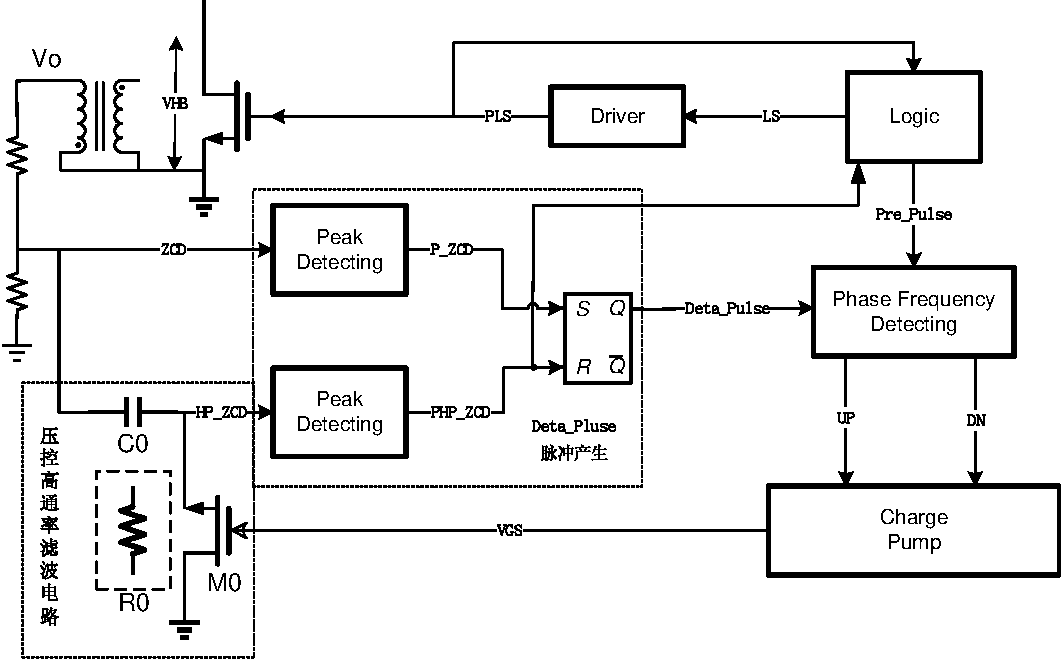
\includegraphics[width=0.8\linewidth]{figures/精确谷底导通电路图1.pdf}
    \caption{精确谷底导通电路图1}
    \label{fig:精确谷底导通电路图1}
\end{figure}


因为功率管半桥节点信号$V_{HB}$的电压值过大,无法直接输入变换器芯片内进行处理,因此对在等待时间$T_w$内同样带有谐振信息的辅助绕组分压引脚ZCD的电压信号$V_{ZCD}$进行采样处理。由于$V_{ZCD}$信号和$V_{HB}$信号的谐振电压相位相反,故$V_{HB}$的谐振谷底对应$V_{ZCD}$的谐振谷峰值。如图~\ref{fig:精确谷底导通电路图1}中所示,采用峰值检测电路来检测$V_{ZCD}$信号在等待时间$T_w$内的谐振谷峰值,并输出对应的峰值脉冲信号P\_ZCD。

峰值检测电路图如图~\ref{fig:峰值检测电路图}所示。峰值检测电路包括一个由晶体管M2、M4、M5、M6和M7组成的五管运算放大器,一个晶体管M9和M10组成的电流镜以及晶体管M11构成的源极跟随器。电流镜晶体管M12为源极跟随器M11提供偏置电流。该电路的工作原理是通过运算放大器比较输入电压$V_{in}$和输出电压$V_{out}$的大小,当输入电压$V_{in}$大于输出电压$V_{out}$时,运算放大器输出低电平,拉低电流镜晶体管M9的栅端电压,电流镜开始工作,对电容$C_1$进行充电,电压$V_1$逐渐升高,$V_{out}$在源极跟随器的作用下也逐渐增大,跟随$V_{in}$变化。当$V_{in}$不再增大,$V_{in}$开始小于$V_{out}$时,运算放大器输出高电平,拉高电流镜晶体管M9的栅端电压,电流镜停止工作,不再给电容$C_1$进行充电,进而输出电压$V_{out}$也保持不变,实现峰值检测的功能。最后通过一个脉冲产生电路输出峰值脉冲信号。同时为了检测在电路在不同周期内不同大小的输入电压$V_{in}$,加入复位开关管M13,当接收到复位信号$R_{st}$后,开关管M13导通,对电容$C_1$进行放电,实现复位的功能。

\begin{figure}[htbp] 
    \centering
    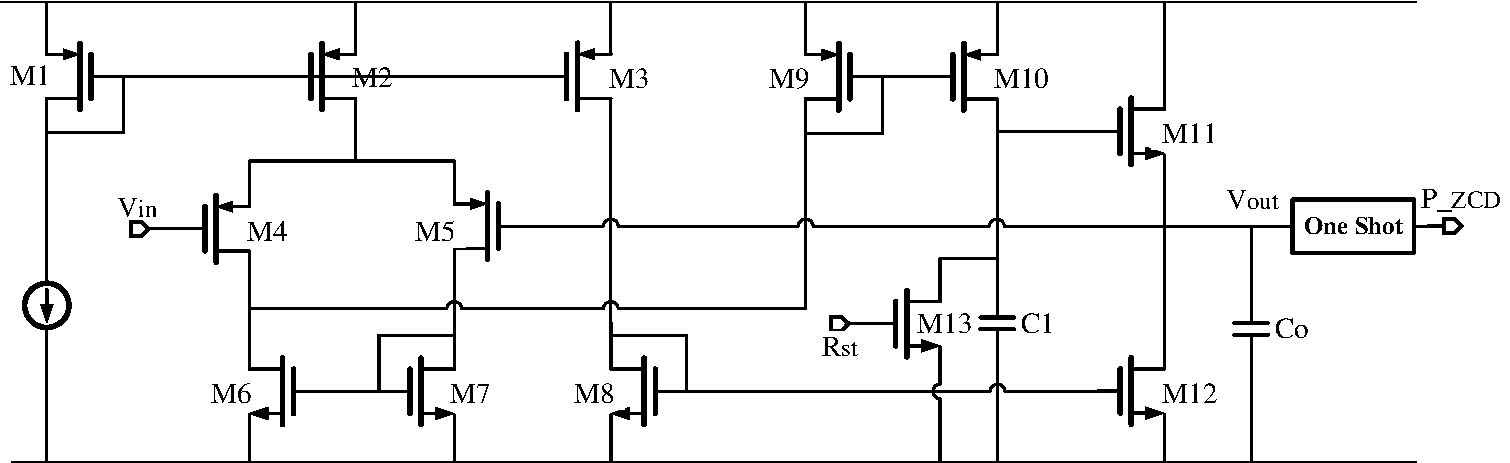
\includegraphics[width=1.0\linewidth]{figures/峰值检测电路图.pdf}
    \caption{峰值检测电路图}
    \label{fig:峰值检测电路图}
\end{figure}

由于驱动电路等电路结构对逻辑控制信号存在延时问题,为了满足精确的谷底导通功能,不能直接将信号$V_{ZCD}$通过峰值检测电路产生的峰值脉冲信号P\_ZCD直接作为时钟信号CLK输入到逻辑控制模块来产生下个开关周期的逻辑控制信号LS。针对于该问题,新颖性地提出了迫使精确谷底导通模块在$V_{HB}$谐振谷底到达之前产生低边功率管的导通时钟信号CLK的方案,使得逻辑控制信号LS通过驱动电路延时后,输出的栅极驱动信号LSGD恰好位于$V_{HB}$信号谐振谷底的位置处,此时导通低边功率管,不仅降低开关损耗,还可以极大地减小峰值检测电压的过冲现象。为满足该功能,要求逻辑控制信号LS超前产生的时间近似等于驱动电路等结构的延时时间。

该模块中实现超前采样$V_{ZCD}$信号峰值的核心电路是采用的压控高通滤波器电路,如图~\ref{fig:精确谷底导通电路图1}中所示,可以通过控制MOS管的栅极电压$V_{GS}$来调节MOS管的导通电阻$R_{on}$,$R_{on}$的计算公式为:
\begin{equation}
    \label{eq:Ron公式}
    R_{on}=\frac{1}{\mu_n C_{ox} \frac{W}{L} (V_{GS} - V_{TH})}
\end{equation}
由式可知,随着MOS管栅极电压$V_{GS}$的增大,其导通电阻逐渐减小。根据高通滤波器的幅频曲线公式可知,当功率管栅压$V_{GS}$为零电压时,功率管截止,导通电阻近似无穷大,对应的时间常数RC无穷大,相位变化为0度,压控高通滤波器的输出信号$V_{ZCD,PH}$和信号$V_{ZCD}$的电压波形重合。随着栅压信号$V_{GS}$的增大,时间RC常数越小,$V_{ZCD,PH}$波形超前的相位变化越大,直至时间常数RC等于零时,超前相位最大值90度。
\begin{equation}
    \label{eq:jw公式}
    \varphi_{j\omega }=\arctan (\frac{\omega_c}{j\omega R C })
\end{equation}
其中$\omega_c$为滤波器的截止频率。通过和合理的调节MOS管栅压信号$V_{GS}$的值,即可调节$V_{ZCD,ph}$波形恰好超前$V_{ZCD}$电压波形的相位时间信号D\_Phase和驱动电路的延时时间信号L\_Phase的脉冲宽度相等,实现低边功率管栅极驱动信号的精确谷底导通功能。其中,如图~\ref{fig:精确谷底导通电路图1},信号D\_Phase是信号$V_{ZCD,PH}$和$V_{ZCD}$通过峰值采样电路分别输出的峰值脉冲信号PH\_ZCD与P\_ZCD经过一个SR锁存器产生的;信号L\_Phase则是将栅极驱动信号LSGD经过电平移位器降为低压后同逻辑控制信号LS经过SR锁存器产生的。

压控高通滤波器的栅压信号$V_{GS}$的调控方式采用了锁相环电路中的鉴相鉴频器和电荷泵结构来动态调节实现。图~\ref{fig:鉴相鉴频器电路图}为该模块使用的鉴相鉴频器电路和电荷泵的电路图。包括两个带复位端的下降沿D触发器和一个与门组成。触发器的D输入端都接高电平保持逻辑"1",触发器1的时钟输入端D\_Phase是信号$V_{ZCD,PH}$和信号$V_{ZCD}$波形的超前相位时间差;触发器2的时钟输入端L\_Phase是逻辑控制信号LS和栅压驱动信号LSGD的延迟时间差。通过这两个D触发器检测D\_Phase和L\_Phase信号的相位时间差信号UP和DN,再通过信号UP和DN控制电荷泵的开关S1和S2,选择对电容$C_{GS}$进行充电或放电功能。

\begin{figure}[htbp] 
    \centering
    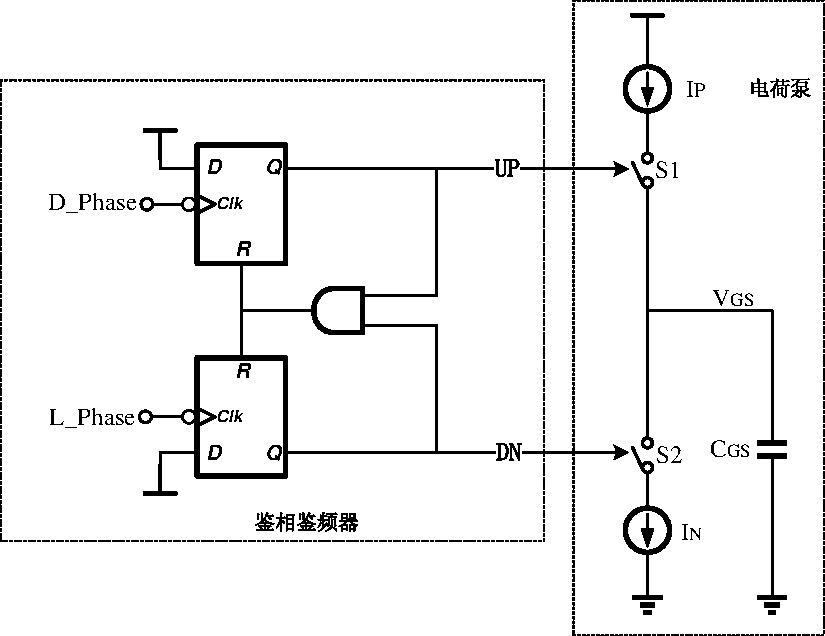
\includegraphics[width=0.6\linewidth]{figures/鉴相鉴频器.pdf}
    \caption{鉴相鉴频器和电荷泵电路图}
    \label{fig:鉴相鉴频器电路图}
\end{figure}

鉴相鉴频器和电荷的波形图如~\ref{fig:鉴相鉴频器波形图}所示。不同于上升沿D触发器组成的鉴相鉴频器,该模块中使用的下降沿鉴相鉴频器的输出信号UP和DN是信号D\_Phase和L\_Phase的下降沿的相位时间差。当信号D\_Phase先于信号L\_Phase变为低电平时,信号UP由低变高,导通开关S1,电流源$I_P$对电容$C_{GS}$进行充电,电压$V_{GS}$逐渐增大;当信号L\_Phase的下降沿到来后,UP由高变低,开关S1关断,$V_{GS}$保持不变。同理,信号DN和UP相似,区别在于L\_Phase先于信号D\_Phase变为低电平时有低变高,导通开关S2通过电流源$I_N$对电容$C_{GS}$进行放电,电压$V_{GS}$逐渐减小。随着鉴相鉴频器和电荷泵电路的不断工作,最终信号D\_Phase和信号L\_Phase几乎重叠,信号UP和DN脉冲保持一致,同时给电容$C_{GS}$进行充电和放电,电压$V_{GS}$维持稳定。

\begin{figure}[htbp] 
    \centering
    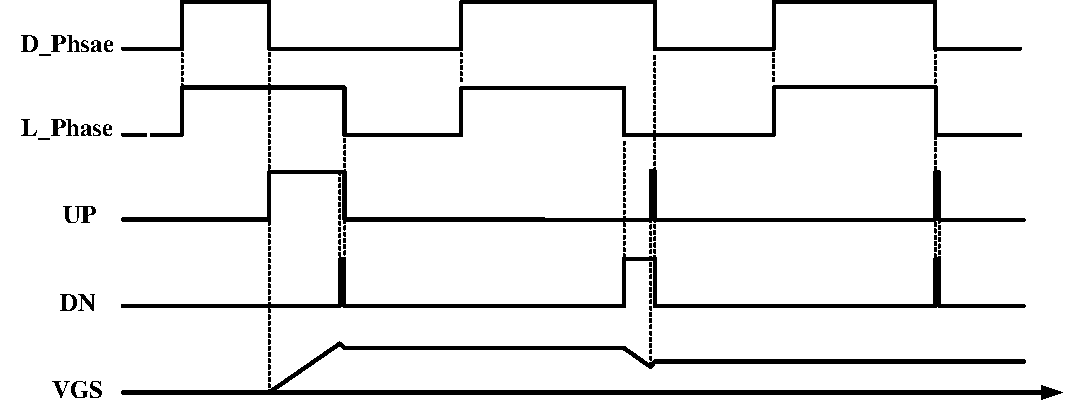
\includegraphics[width=0.8\linewidth]{figures/鉴相鉴频器波形图.pdf}
    \caption{鉴相鉴频器电荷泵波形图}
    \label{fig:鉴相鉴频器波形图}
\end{figure} 

其中,模块中使用的单端结构电荷泵的实际电路图如图~\ref{fig:电荷泵电路图}所示,电荷泵的单端结构占用面积较小,且更易于设计,满足于精确谷底导通模块的使用需求。同时为了减小电荷泵电路中的电荷注入、时钟馈通和电荷共享的非理性效应,采用了源极开关型结构。该电荷泵结构未直接将MOS开关管MP5、MN4连接在电容$C_{GS}$的上极板,通过电流镜晶体管MP6、MN3将开光管和电容隔离开,阻挡了开关管关断时反型层中的沟道电荷注入电容,提高了电压$V_{GS}$的稳定性。

\begin{figure}[htbp] 
    \centering
    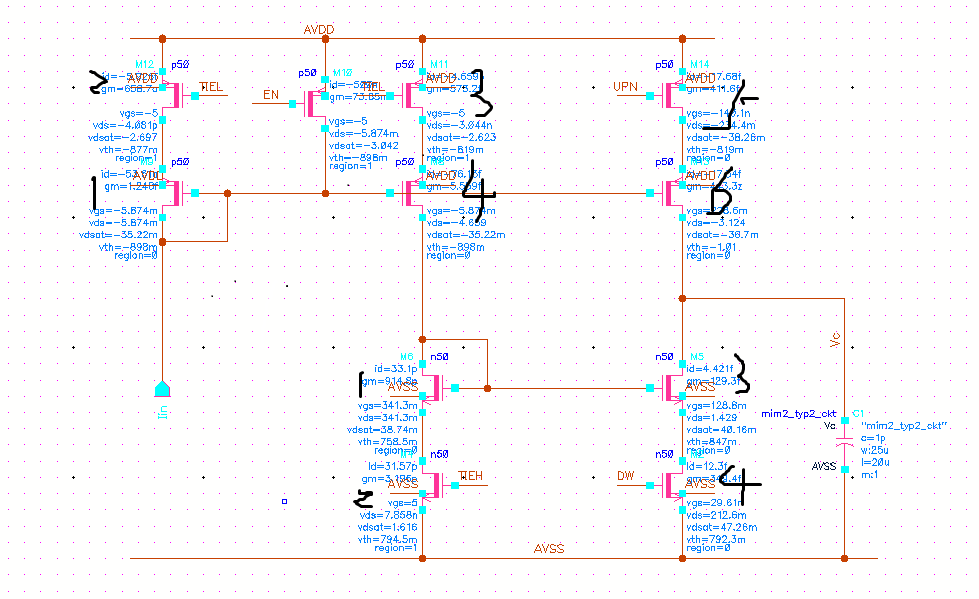
\includegraphics[width=0.8\linewidth]{figures/电荷泵电路图.png}
    \caption{电荷泵电路图}
    \label{fig:电荷泵电路图}
\end{figure} 

为了满足PMOS管在信号UP的控制下正确地导通和关断,通过一个反相器输出信号UPN来控制开关管MP5,在信号UP电压由低变高时,信号UPN电压由高变低,导通开关管MP5,对电容$C_{GS}$进行充电;信号DN电压由低变高时,直接控制开关管MN4导通,对电容$C_{GS}$进行放电。电荷泵电路除了由晶体管MP1、MP4、MP6组成的PMOS电流镜和晶体管MN1、MN3组成的NMOS电流镜,还额外加入了晶体管MP2、MP3、MN2来和开关管MP5 MN4相对应,提高了电路的对称性,在开关管导通时使得电流镜晶体管的源极电压相等,提高电流镜的复制比精度,迫使电容$C_{GS}$的充放电电流尽可能一致。


结合图~\ref{fig:精确谷底导通波形图}中的工作波形,精确谷底导通模块的具体工作过程为:当工作模式首次切换为RVS模式时,此时压控高通滤波器的栅压$V_{GS}$为零,晶体管M0未导通,晶体管的导通电阻近似无穷大,高通滤波器的相位变化为零,信号$V_{ZCD,PH}$和信号$V_{ZCD}$波形重叠,模块将峰值检测电路检测的$V_{ZCD}$峰值脉冲信号P\_ZCD作为时钟CLK输出给逻辑控制模块,产生的逻辑控制信号LS在t1时刻的$V_{HB}$谐振谷底处由低电平变为高电平,经过驱动电路延时后,栅极驱动信号在t2时刻控制低边功率管导通,此时$V_{HB}$电压较大,产生较大的开关损耗。信号D\_Phase和L\_Phase经过鉴相鉴频器输出的信号UP导通电荷泵开关管对电容充电,压控高通滤波器栅压$V_{GS}$线性增大。

\begin{figure}[htbp] 
    \centering
    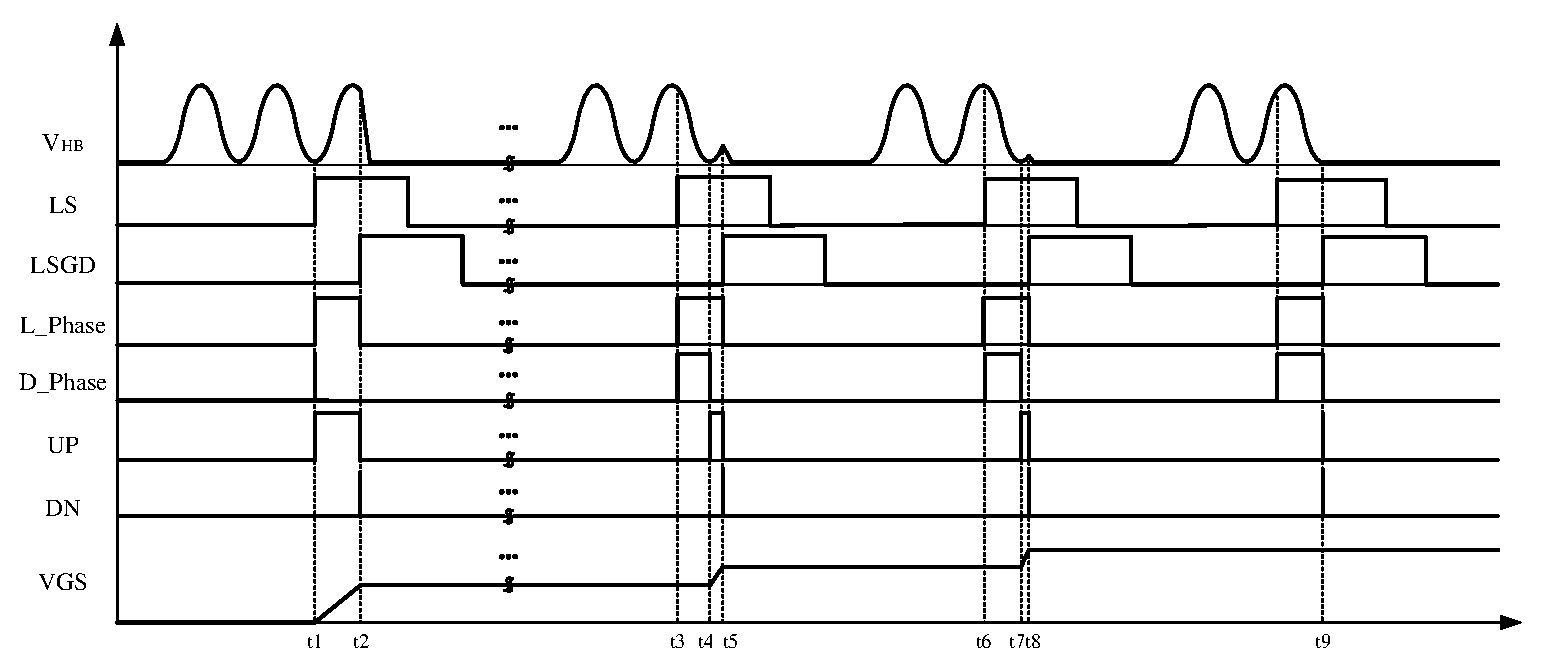
\includegraphics[width=1.0\linewidth]{figures/精确谷底导通波形图.pdf}
    \caption{精确谷底导通电路相关波形图}
    \label{fig:精确谷底导通波形图}
\end{figure} 

经过几个开关周期的充电后,栅压$V_{GS}$大于晶体管M0阈值电压,晶体管导通,压控高通滤波器产生的超前信号D\_Phase迫使信号LS在$V_{HB}$谐振谷底前导通,与信号L\_Phase之间的相位差UP也相应减小,成功实现逐步逼近功能,栅极驱动信号LSGD在t5时刻导通低边功率管,此时虽仍未在谷底处导通,但开关损耗已大大降低。

最后经过几个开关周期的变化,压控高通滤波器产生的超前信号D\_Phase几乎与信号L\_Phase重叠,鉴相鉴频器输出信号UP和DN脉冲宽度相等,电容上电压$V_{GS}$维持稳定,t9时刻LSGD在$V_{HB}$谐振谷底处实现精确导通低边功率管的功能。

\subsection{精确谷底导通电路仿真分析}

\begin{figure}[htbp] 
    \centering
    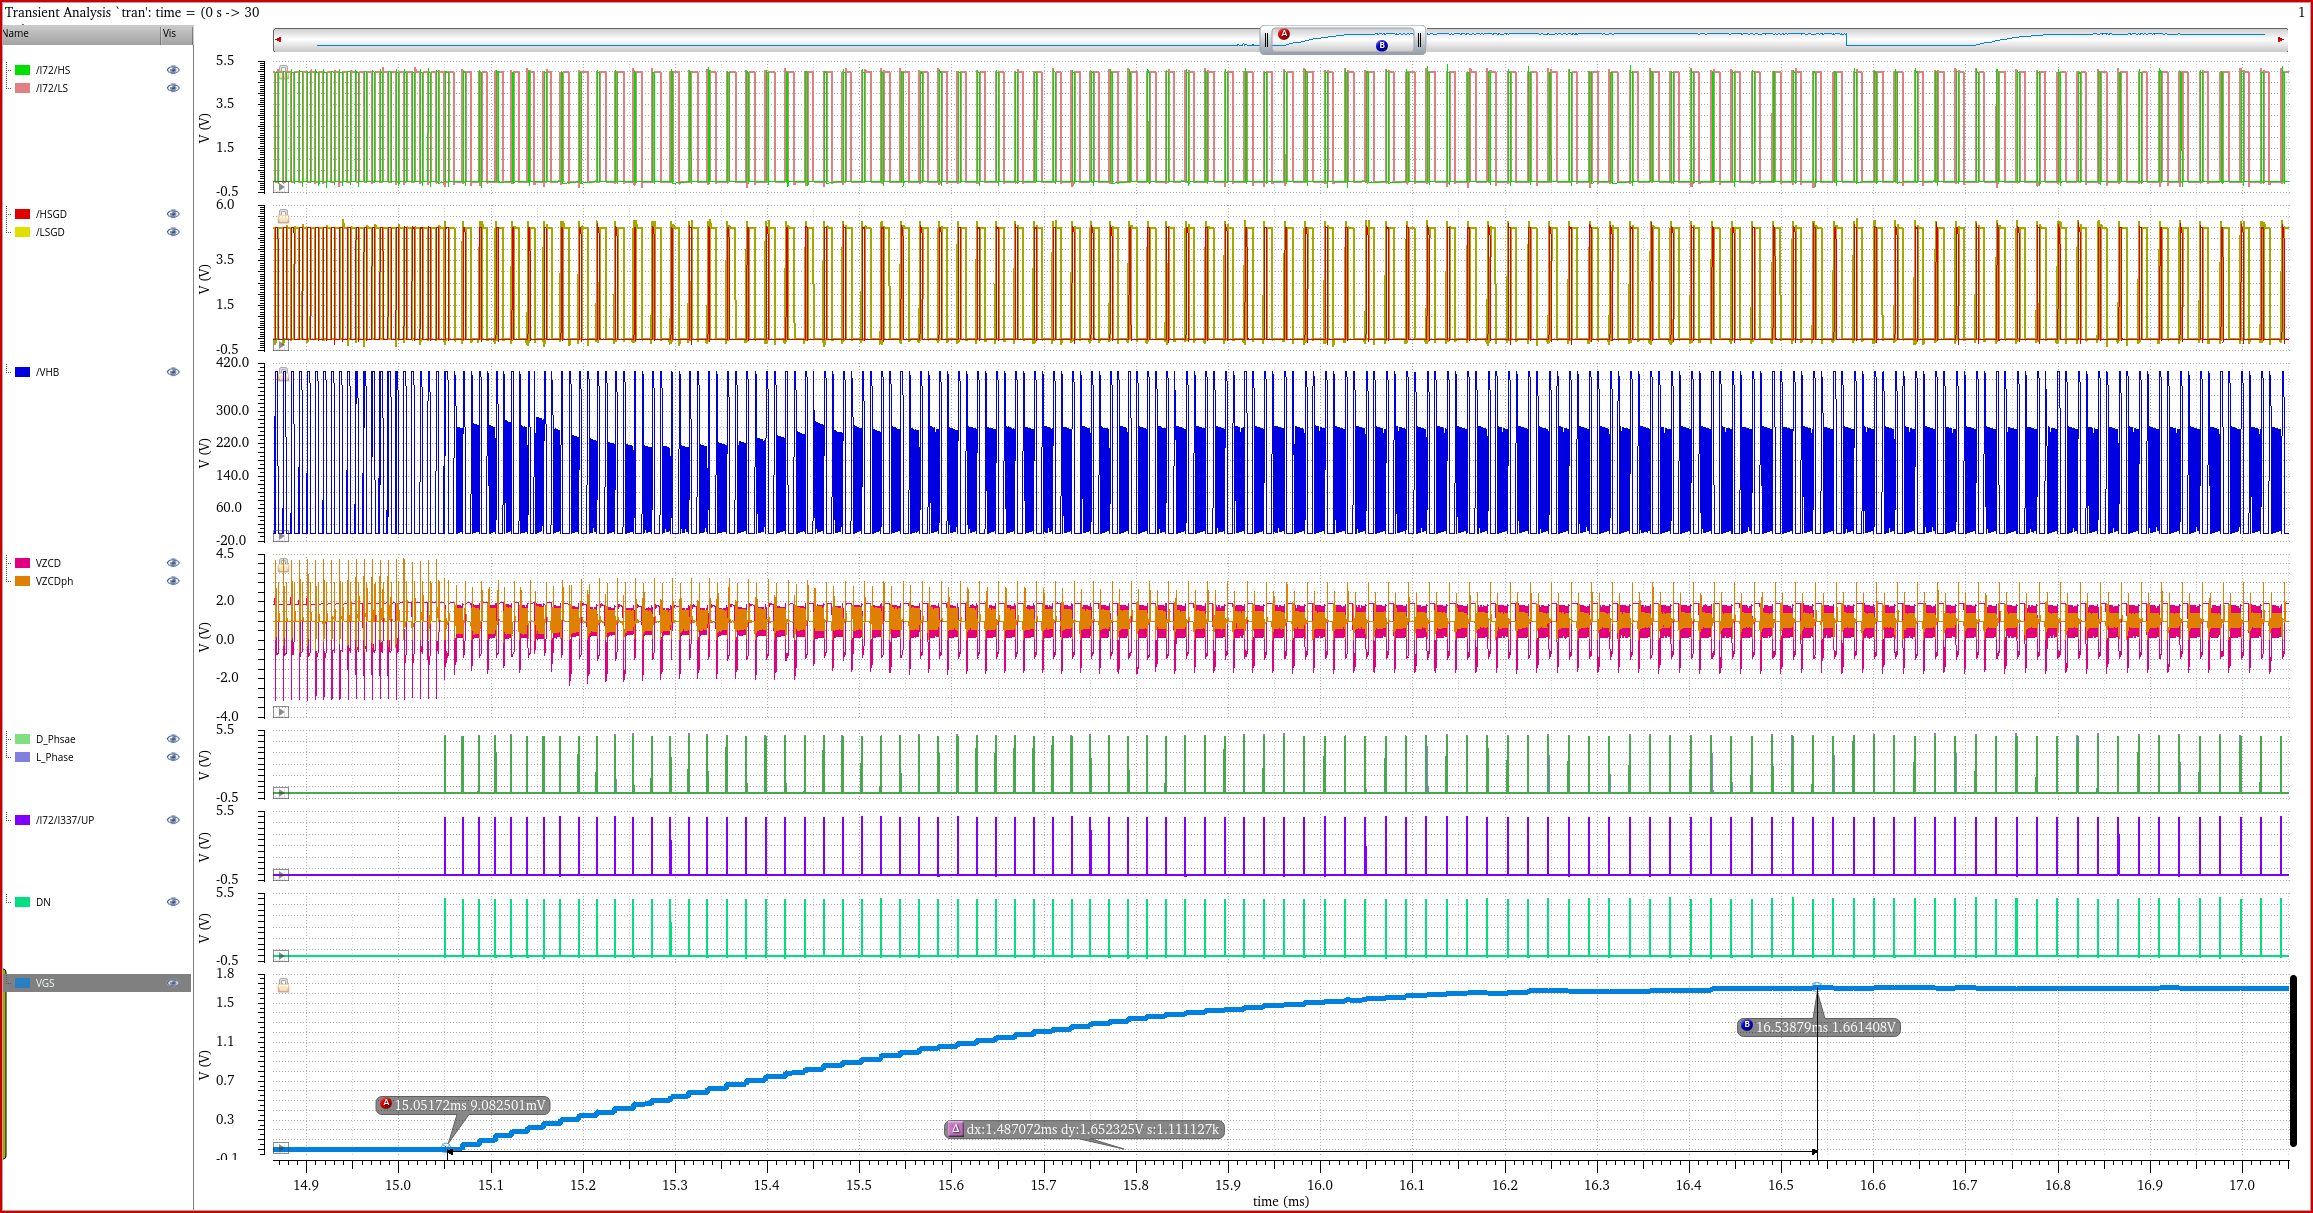
\includegraphics[width=0.8\linewidth]{figures/valley_switch.png}
    \caption{精确谷底导通电路相关波形仿真图}
    \label{fig:谷底导通仿真图}
\end{figure} 


\begin{figure}[htbp]
	\centering
	\subcaptionbox{未稳定\label{fig:谷底导通仿真图1}}{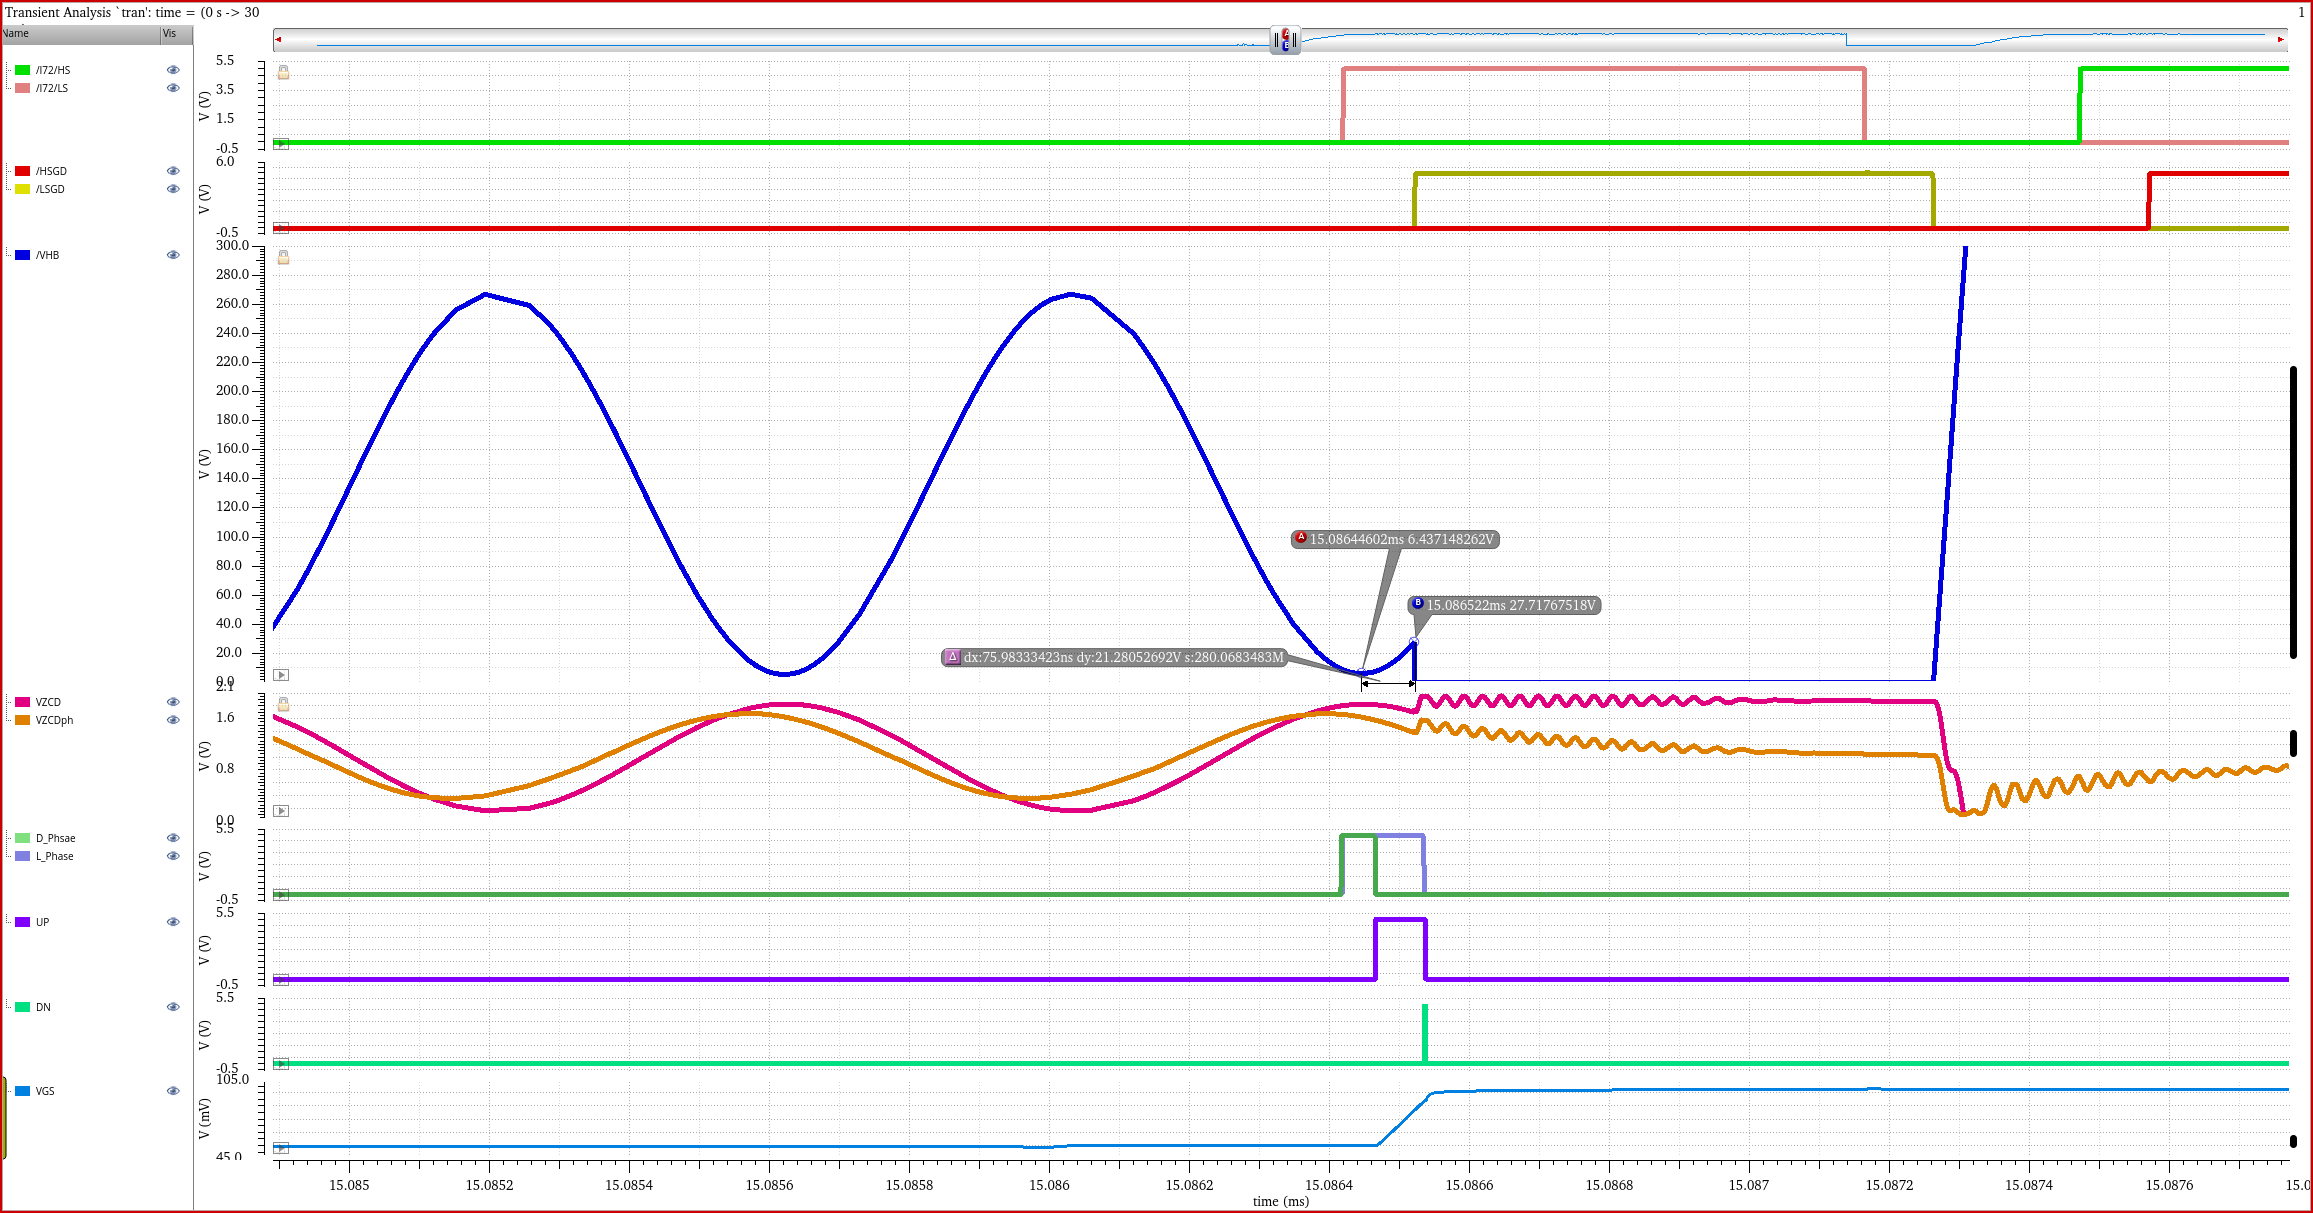
\includegraphics[width = 0.45\linewidth]{figures/valley_switch1.png}}
	\subcaptionbox{稳定\label{fig:谷底导通仿真图2}}{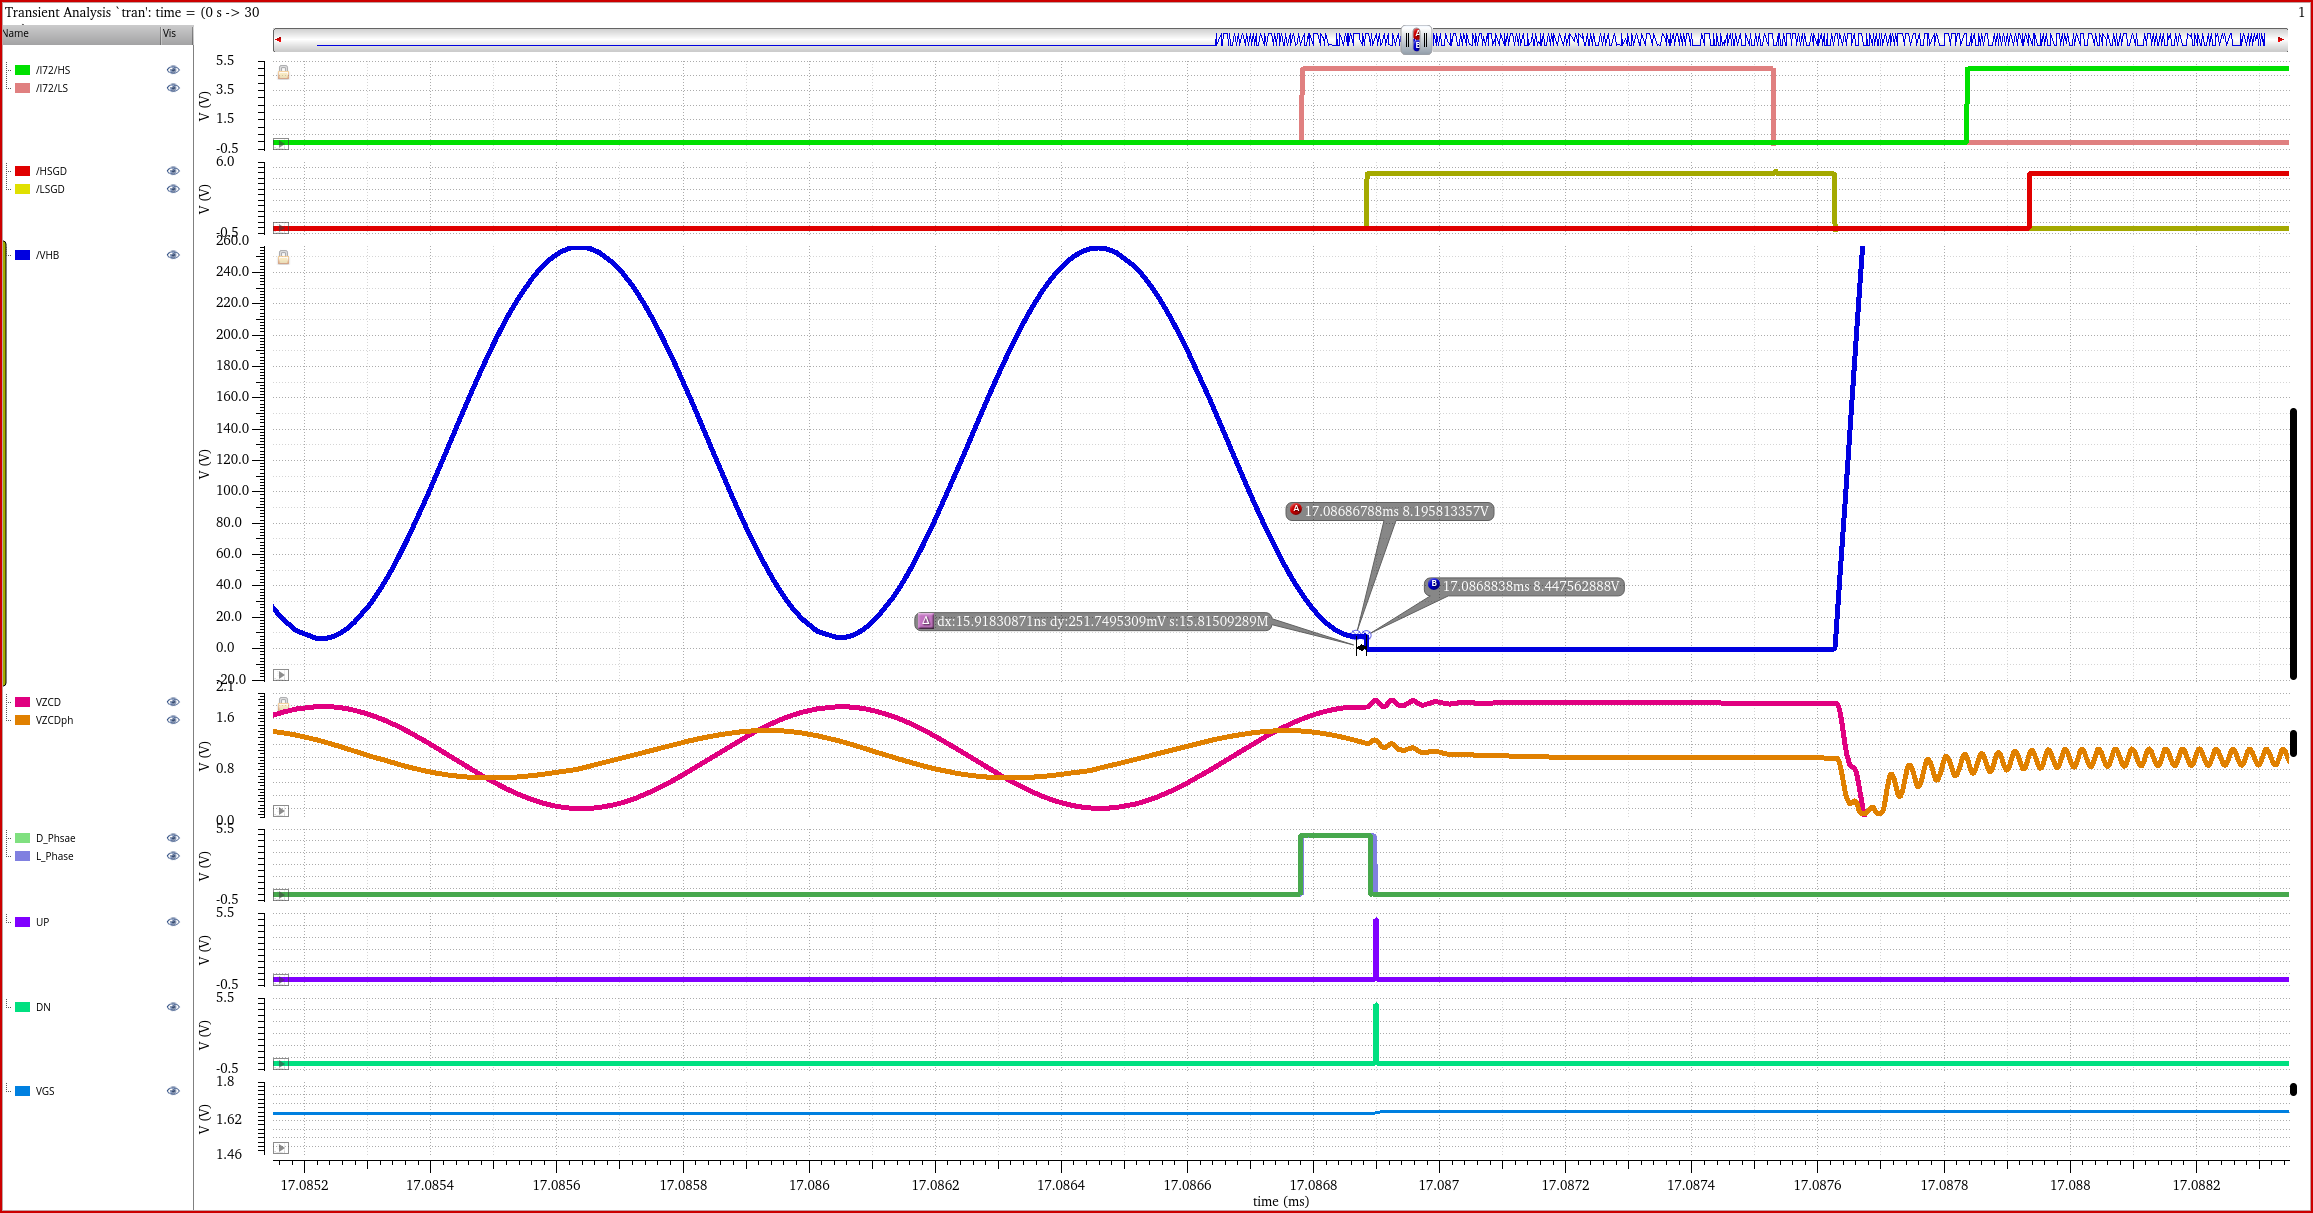
\includegraphics[width = 0.45\linewidth]{figures/valley_switch2.png}}
	\caption{谷底导通放大仿真图}
	\label{fig:谷底导通放大仿真图}
\end{figure}

图~\ref{fig:谷底导通仿真图}为精确谷底导通电路相关波形仿真图,由仿真图可见,当系统由恒流模式切换为恒压模式中的RVS工作模式后,精确谷底导通模块内压控高通滤波器的栅压$V_{GS}$随着开关周期逐渐增大,经过1.43ms后稳定在1.65V,此时电路已完成精确谷底导通功能。图~\ref{fig:谷底导通放大仿真图}中分别展示了电路在栅压$V_{GS}$未稳定和稳定后的具体波形图。在图~\ref{fig:谷底导通放大仿真图} (a)中,栅极驱动信号LSGD未能在$V_{HB}$谐振谷底处导通,其导通时刻$V_{HB}$电压值等于27.7V,和谷底处电压值的差值约为21.3V。在图~\ref{fig:谷底导通放大仿真图} (b)中可见,由于电路精度的限制,栅极驱动信号LSGD导通低边功率管时$V_{HB}$电压值和谷底电压值的差值仅为252mV,可以近似忽略不计,实现了电路的设计需求和功能。

%通过逻辑控制电路得到LS和PLS信号的延时时间Pre\_Pulse。为了预判谷底信号,通过一个使用MOS管充当电阻的压控高通滤波器电路,产生$V_{ZCD}$对应的超前时间信号VHP\_ZCD,只需适当的调节VGS的大小即可控制VHP\_ZCD信号的超前时间大小。分别使用两个峰值检测电路来检测并得到两个信号的峰值脉冲信号,经过SR锁存器产生超前时间Deta\_Pulse。为了轻微的调节栅极电压信号VGS,使用了PLL电路中的鉴相鉴频器和电荷泵电路来控制Deta\_Pulse信号逐步逼近Pre\_Pulse信号,完成低边功率管的精确谷底导通功能。




\section{谷值锁定电路}

\subsection{谷值锁定电路原理}

在RVS工作模式中,上文所提到的精确谷底导通电路工作前需先确认等待时间信号$T_w$,只有识别到$T_w$的下降沿到达后,才能在其之后的谐振谷底处导通低边功率管,如图~\ref{fig:谷值锁定波形1}所示,当t1时刻$T_w$电压由高变低后,精确谷底导通模块开始工作,寻找识别到距离下降沿最近的t2时刻的谐振谷底,开启下个开关周期。

\begin{figure}[htbp] 
    \centering
    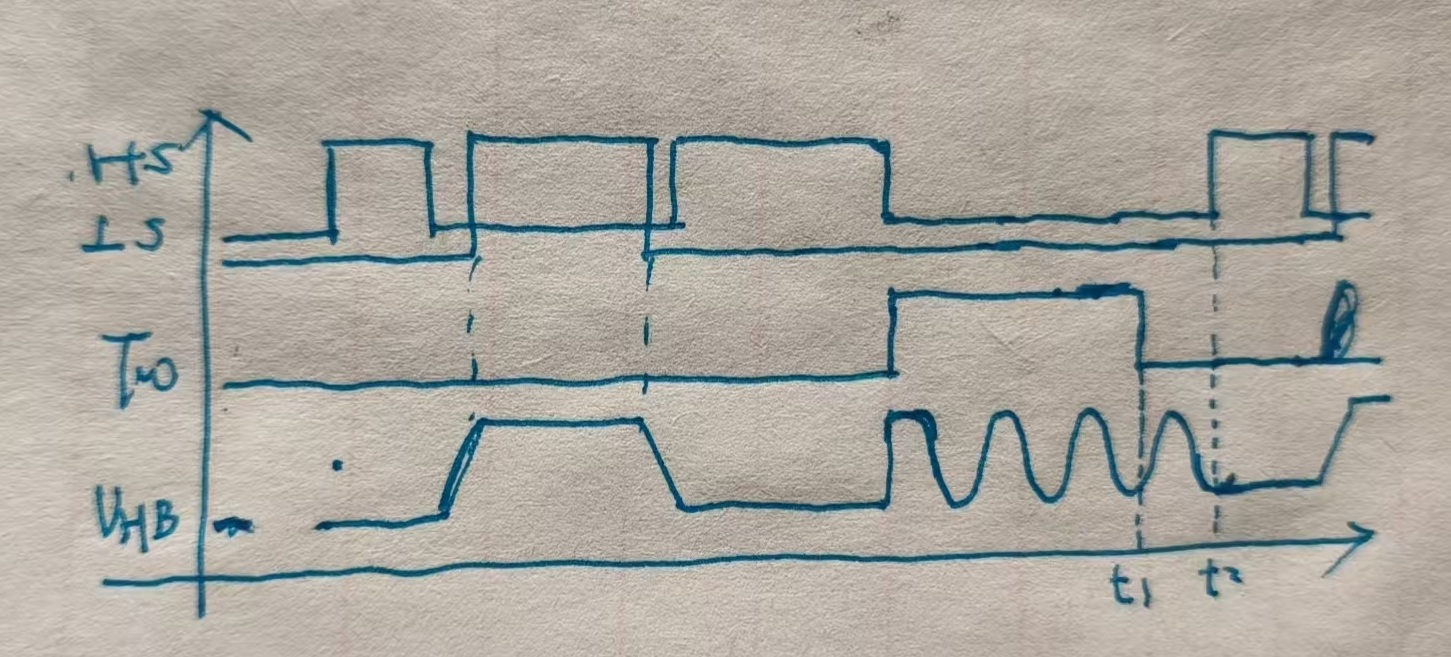
\includegraphics[width=0.6\linewidth]{figures/谷值锁定波形1.jpg}
    \caption{谷值锁定波形1}
    \label{fig:谷值锁定波形1}
\end{figure} 

若使用随负载变化控制频率大小的振荡器电路来产生$T_w$,可能会出现在功率重叠范围内即使输出负载不变,$T_w$内信号$V_{HB}$的谐振谷数值在不同开关周期内发生来回跳动的情况,称之为跳谷现象,为解决该问题,设计了谷值锁定电路。

谷值锁定电路的作用同样是根据负载的轻重情况调节开关频率大小,副边反馈引脚电压信号$V_{FB}$如~\ref{sec:峰值电流控制电路}小节中提到的,是峰值电流参考电压$V_{CSP}$的重要组成部分,可以一定程度地反映输出负载电流的大小。为了降低导通损耗,需要维持一个较低的峰值电流,因此在负载变化时,利用谷值锁定电路根据$V_{FB}$的变化动态调节谐振谷的数量,以改变$T_w$时间长度的方式改变开关频率,更快地恢复输出电压的稳定。
但不同与振荡器电路的是,为了防止跳谷现象的产生,通过对负载的变化调整并锁定等待时间$T_w$内的谐振谷数值,只有当电路判断实际的谷值和设定谷值相等时,才允许精确谷底导通模块在最近的谷底处导通低边功率管,开启下一开关周期。该电路彻底避免了在负载不变的情况下谐振谷值的频繁变化问题,减小了电路的不稳定现象。

谷值锁定电路具体组成如图~\ref{fig:谷值锁定电路1}所示,主要包括三个迟滞比较器、一个D触发器、一个单向计数器、一个双向计数器和DAC电路等。
%该电路的设计原理是,当输出负载电流较小时,$V_{FB}$的电压值也较小,此时谷值锁定电路增大$T_w$时间内的谐振谷值,降低开关频率。

\begin{figure}[htbp] 
    \centering
    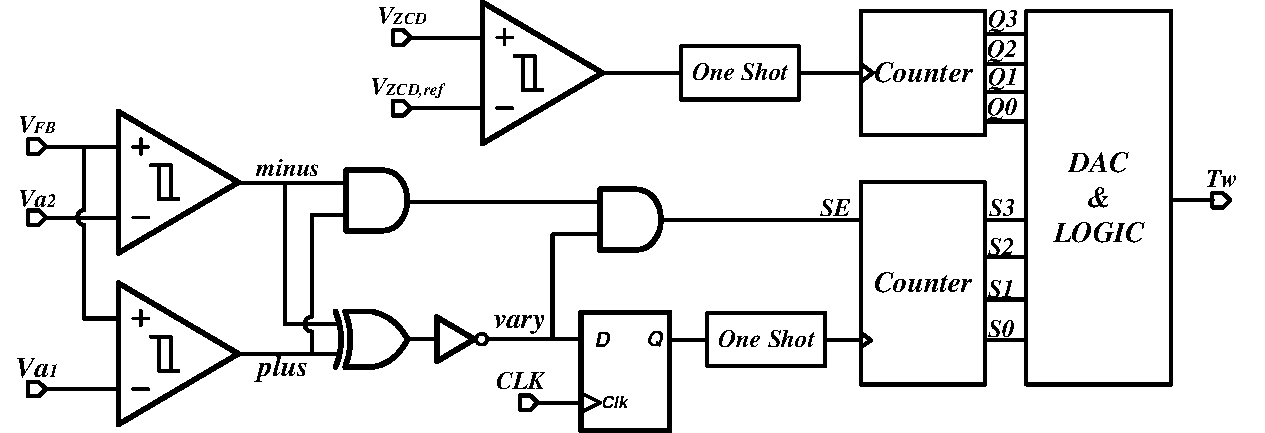
\includegraphics[width=0.8\linewidth]{figures/谷值锁定电路1.pdf}
    \caption{谷值锁定电路1}
    \label{fig:谷值锁定电路1}
\end{figure} 

如图~\ref{fig:谷值变化策略}的谐振谷数值变化策略所示,当输出负载电流较小时,$V_{FB}$电压值小于参考电压Va1,比较器3的输出端plus等于逻辑“1”,此时需要随着CLK信号的触发通过双向计数器电路增加$T_w$时间内的谐振谷数量,降低开关频率;当输出负载电流较大时,$V_{FB}$电压值大于参考电压Va2,比较器2的输出端minus等于逻辑“1”,说明需要减小$T_w$时间内的谐振谷数量,增大开关频率;当$V_{FB}$大于Va1但小于Va2时,锁定$T_w$时间内的谐振谷数量,防止发生跳谷现象。

\begin{figure}[htbp] 
    \centering
    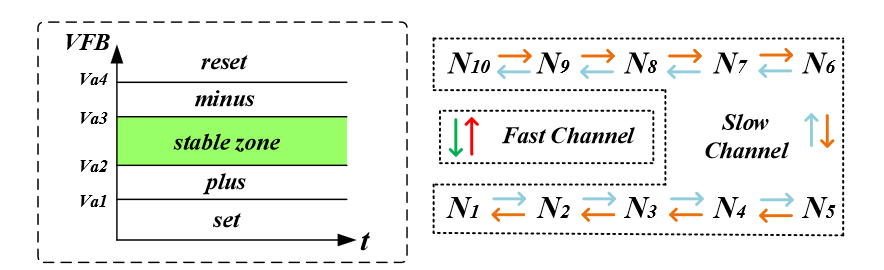
\includegraphics[width=0.8\linewidth]{figures/谷值变化策略.png}
    \caption{谷值变化策略图}
    \label{fig:谷值变化策略}
\end{figure} 

信号$V_{FB}$和参考电压Va1、Va2通过比较器比较后输出的信号plus、minus的组合逻辑决定了谷值锁定电路不同的工作状态,具体工作状态如~\ref{tab:谷值锁定电路}表所示。如在plus信号为逻辑“0”,minus信号为逻辑“1”时,谷值锁定电路将对谐振谷数量进行锁定;在plus和minus信号的其他逻辑转态将对谐振谷进行增加或减小数量的调整操作。plus和minus信号通过一个同或门后输出vary信号并连接到D触发器的D输入端,保证在vary信号为逻辑“1”时允许时钟信号CLK对双向计数器进行计数。plus和minus信号还经过两个与门后输出SE信号,SE信号控制了双向计数器向上和向下的两种计数模式。当SE信号为逻辑“1”时,双向计数器进行向上计数操作,增加$T_w$时间内的谐振谷数量;当SE信号为逻辑“0”时,双向计数器进行向下计数操作,减少$T_w$时间内的谐振谷数量。双向计数器输出的4bit信号S[3:0]会通过DAC电路转为模拟电压信号,与另一个计数器产生的4bit信号Q[3:0]产生的电压信号进行比较,输出$T_w$等待时间给精确谷底导通电路。

其中CLK脉冲信号的设置根据香农定律,为了保证信号采样的完整性,采样频率应至少为带宽的两倍。本文定义$\frac{1}{T_{CLK}}$作为CLK脉冲信号的工作频率。在开关电源系统中,为了避免可听噪声,开关频率$f_{CLK}$必须超过20Hz ~ 20KHz频段。$T_{CLK}$可以表示为如下形式:
\begin{equation}
    \label{eq:CLK公式}
    T_{CLK} > 2 \times \frac{1}{20kHz}
\end{equation}
取$T_{CLK}$的开关周期长度为100u。


%为了防止出现如前文~\ref{sec:多模式切换}小节中提到的峰值电流和开关频率同时变化引起的相位裕度降低和电路不稳定情况,轻载时采取的RVS工作模式通过改变开关频率的方式维持峰值电流的基本恒定。副边反馈引脚电压信号$V_{FB}$如~\ref{sec:峰值电流控制电路}小节中提到的,是峰值电流参考电压$V_{CSP}$的重要组成部分,可以一定程度地反映输出负载电流的大小。当负载电流突然增大时,为了满足变大的输出功率,变压器原边需要增大高边功率管的导通时间提供更多的能量给输出电容,因此$V_{CSP}$增大,$V_{FB}$也相应地增大;当负载电流突然减小时,同理$V_{FB}$也会相应地减小。同时为了降低导通损耗,需要维持一个较低的峰值电流,因此在负载波动时,利用谷值锁定电路通过随$V_{FB}$变化动态调节谐振谷的数量,改变$T_w$时间长度的方式改变开关频率,更快地恢复输出电压的稳定。



\begin{table}[htbp]
    \caption{谷值锁定的三种操作}
    \label{tab:谷值锁定电路}
    \centering
    \belowrulesep=0pt  %防止竖线不连续
    \aboverulesep=0pt  %防止竖线不连续
        \begin{tabular}{|c|c|c|c|c|}
            \toprule
             (minus,plus) & 功能 & vary & SE \\
            \midrule
             (0,0)  & 减小谷值  & 1 &    0                   \\  \midrule
             (0,1)  & 锁定谷值  & 0 & disable                \\  \midrule
             (1,1)  & 增加谷值  & 1 &    1       \\          
            \bottomrule
        \end{tabular}
\end{table}

4bit双向计数器电路的电路图如图~\ref{fig:双向计数器电路}所示,包括四个D触发器和MUX电路。不同于普通的单向计数器,可以通过SE信号选择实现向上或向下计数的功能。当SE信号为逻辑“1”时,将每个D触发器的反向输出端输入到下一个D触发器的CLK输入端,此时是向上计数功能;当SE信号为逻辑“0”时,MUX将D触发器的正向输出端输入到下一个D触发器的CLK输入端,实现向下计数功能。电路中还包括hold信号,hold信号的作用是消隐掉SE信号的电平切换的上升沿或下降沿,防止其对计数方向切换造成影响。

\begin{figure}[htbp] 
    \centering
    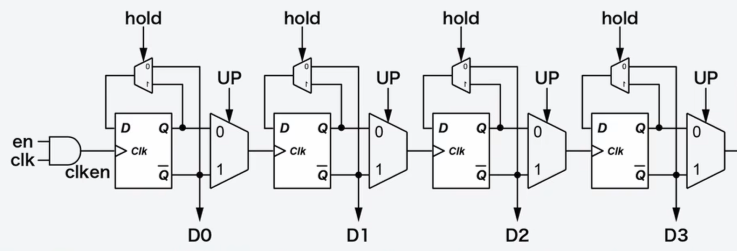
\includegraphics[width=0.8\linewidth]{figures/双向计数器电路.png}
    \caption{双向计数器电路图}
    \label{fig:双向计数器电路}
\end{figure} 

谷值锁定电路中的DAC电路如图~\ref{fig:双向计数器电路}所示,计数器的计数值作为DAC的输入信号,两个计数器分别控制思路电流镜开关管的导通和关断,每个电流镜的镜像比例为1:2:4:8,成倍增加,产生随4bit数字信号S[3:0]、Q[3:0]信号对应的电流$I_S$、$I_Q$。电流镜采用了cascode结构增大电流镜的输出阻抗,提高电流镜像的精度。每一路电流镜还都添加了毛刺消除结构晶体管M11、M13等,用于吸收当数字信号控制M10、M12等开关管导通瞬间产生的巨大毛刺电压。
没有毛刺消除结构时,如图~\ref{fig:双向计数器电路}中的电压V2和V3,分别为晶体管M2和M3的漏极电压,在数字信号S0未导通开关管M10时,$V_2=V_3=V_{DD}$;当S0控制开关管M10导通,电压V3由于cascode结构的大输出阻抗的作用下和电压V1近似相等,电压V2则由于开关管导通等于电阻$R_S$上的电压。在开关管通断前后电压V2和V3的变化量分别为:
\begin{equation}
    \label{eq:△V2公式}
    \varDelta V_2 = V_{DD} - V_{GS1}
\end{equation}
\begin{equation}
    \label{eq:△V3公式}
    \varDelta V_3 = V_{DD} - V_S
\end{equation}

由于电流镜晶体管存在寄生电容$C_{ds}$,故电流镜晶体管M3和M2的寄生电容上的能量$\varDelta P_3 = \varDelta V_3 C_{ds3}$、$\varDelta P_2 = \varDelta V_2 C_{ds2}$会在开关管导通的瞬间传递到电阻$R_S$上,在电压$V_S$引起巨大的毛刺。加入毛刺消除结构M11后,由于M11是NMOS晶体管,其会和开关管M10交替导通,在晶体管M11导通时,电压V2等于零,电压V3的值仍近似等于V1;当开关管M10导通的时候,电压V2和V3的值和没有晶体管M11时相同,故电压V2和V3的变化量分别变为:
\begin{equation}
    \label{eq:△V2公式1}
    \varDelta V_2 = V_{GS1} - V_{GS1} = 0
\end{equation}
\begin{equation}
    \label{eq:△V3公式1}
    \varDelta V_3 = V_S - 0 = V_S
\end{equation}
由式中可见得,电压V2和V3的变化量大大降低,明显降低了毛刺现象。

\begin{figure}[htbp] 
    \centering
    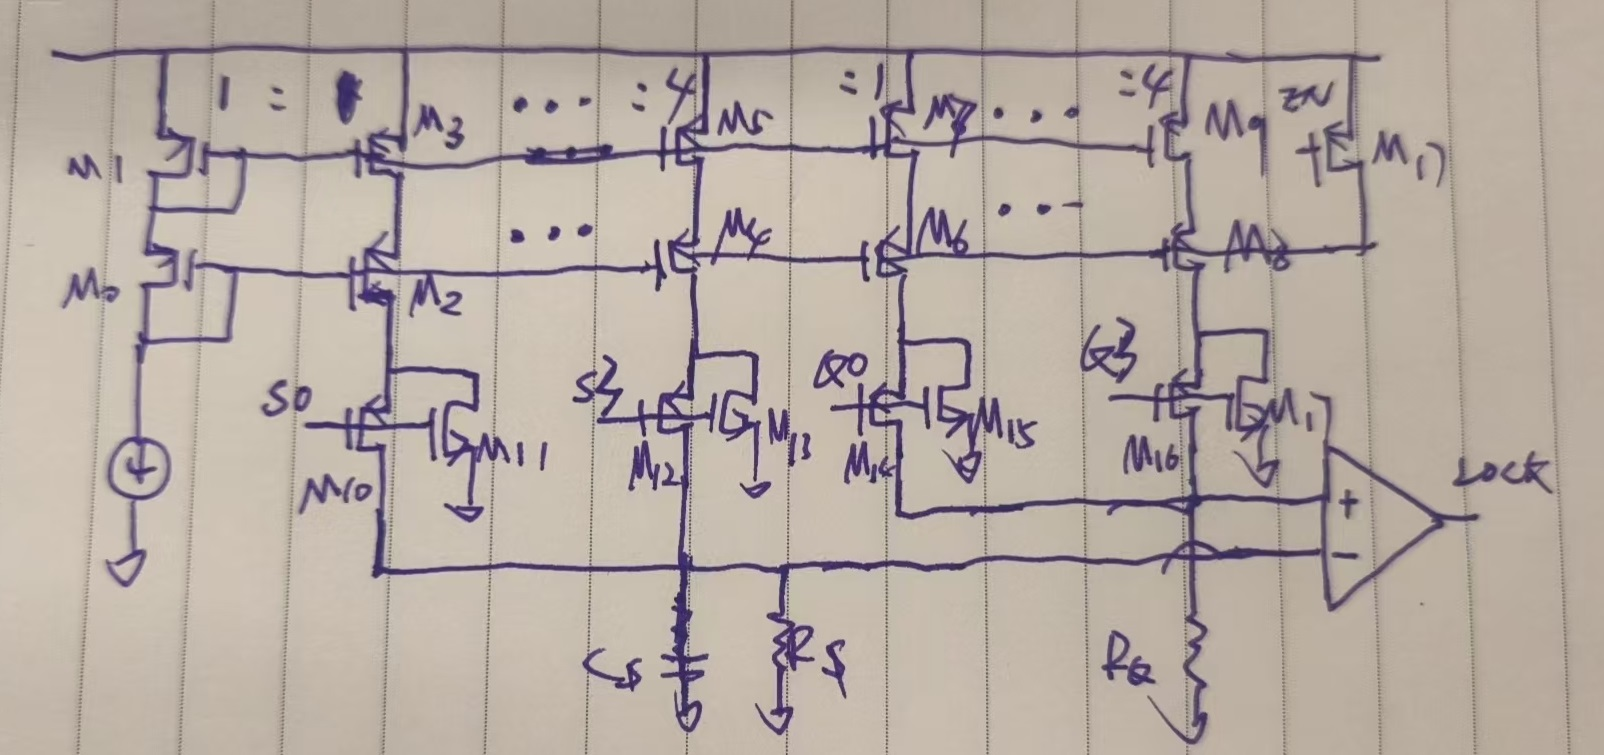
\includegraphics[width=0.6\linewidth]{figures/DAC电路.jpg}
    \caption{DAC电路图}
    \label{fig:DAC电路}
\end{figure} 

数字信号S[3:0]、Q[3:0]控制产生的电流$I_S$、$I_Q$流经电阻$R_S$、$R_Q$后产生的电压$V_S$、$V_Q$通过比较器进行比较大小,当电压$V_Q$大于$V_S$后,比较器输出信号$T_w$由高电平转为低电平,锁定时间结束,精确谷底导通电路开始工作,寻找最近的谐振谷底开启下一开关周期。

\subsection{谷值锁定电路仿真分析}

图~\ref{fig:单周期谷值锁定电路波形图}为单个开关周期内的谷值锁定电路相关的波形图,图中在t1时刻处,原边励磁电感退磁完成,低边功率管顺势关断,此时进入等待时间$T_w$内,图中$T_w$的波形由低电平变化为高电平,在经过一段时间在t2时刻原边电流恢复到零安培后,半桥节点电压信号$V_{FB}$和辅助绕组分压信号$V_{ZCD}$开始自由振荡,通过比较$V_{ZCD}$和$V_{ZCD,ref}$,计数器1不断地对谐振谷进行计数,通过DAC电路输出为电压信号$V_{Q}$,在图中可见在t3、t4、t5等时刻电压$V_{Q}$的波形持续进行阶梯式的抬升,直至在t10时刻大于电压信号$V_{S}$,完成信号$V_{S}$设置的对八个谷值的锁定功能,$T_w$的波形也随着由高电平变化为低电平,谷底导通电路接收到此下降沿后,在t11时刻的第八个谐振谷底处开启下一个开关周期。

\begin{figure}[htbp] 
    \centering
    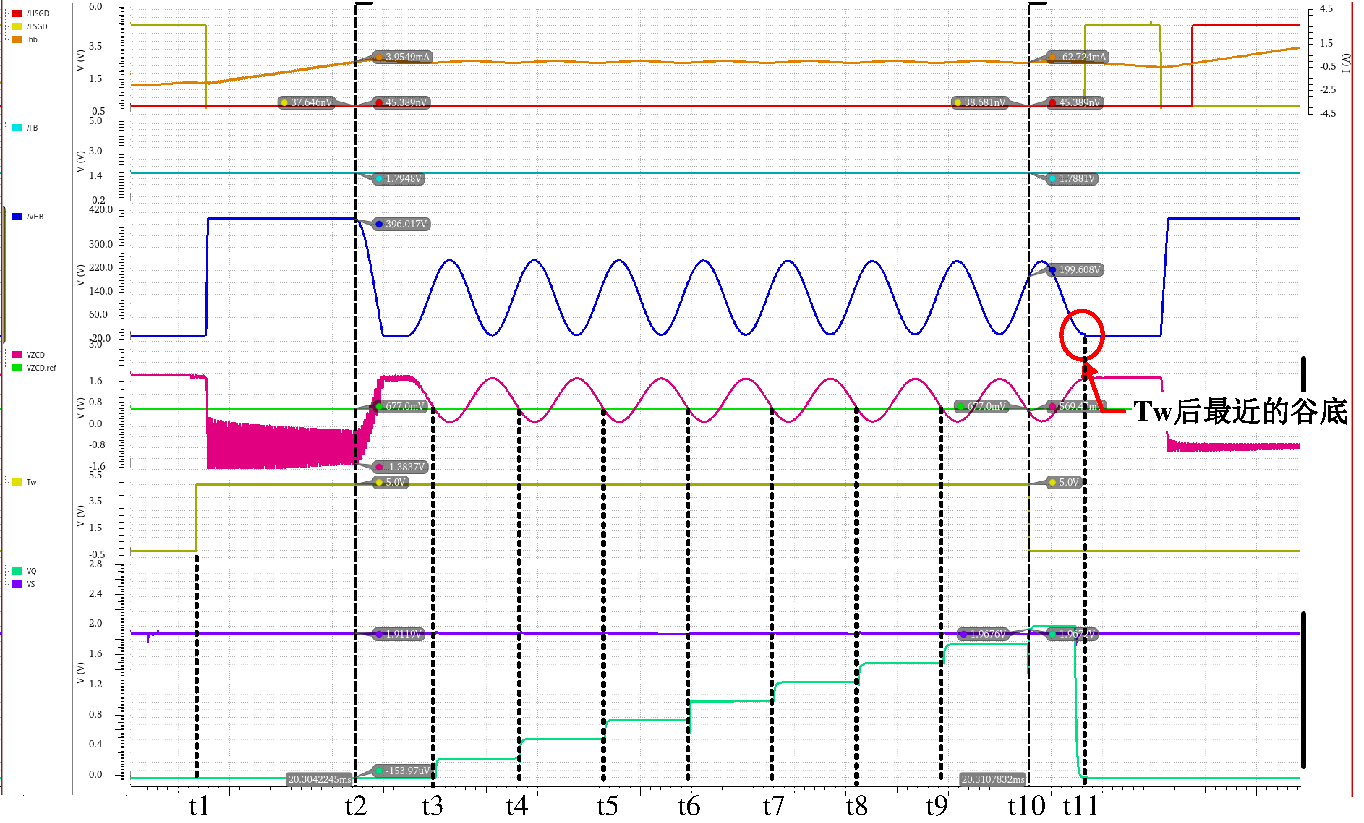
\includegraphics[width=0.8\linewidth]{figures/valley_lock.pdf}
    \caption{单周期谷值锁定电路波形图}
    \label{fig:单周期谷值锁定电路波形图}
\end{figure} 

图~\ref{fig:多周期谷值锁定电路波形图}为多个开关周期内的谷值锁定电路相关的波形图,输出负载电流在图中从1A在t1时刻变化为1.5A,在t5时刻再次变化2A。随着输出负载电流的变化,信号$V_{FB}$的波形如上文所提到的,跟随着发生变化。在t1时刻前,$V_{FB}$小于参考电压$V_{a1}$,此时图中的信号vary为逻辑“1”的高电平,信号SE为逻辑“0”的低电平,表示此时计数器应该随着信号CLK的脉冲增加谐振谷数值,但由于此时图中谐振谷数值已经达到最大谷值,故参考电压$V_S$未发生变化保持恒定的3.15V。
在t1时刻后,负载电流增大为1.5A,在开关频率未变化的情况下,$V_{FB}$为满足输出功率的需求,迅速增大,在t3时刻爬升到大于参考电压$V_{a2}$,信号vary为逻辑“1”,信号SE同样为逻辑“1”,此状态计数器应减少谐振谷数值,在t3和t4时刻之间,随着CLK的脉冲信号电压$V_S$阶梯式降低,开关周期每100us缩短一个谐振谷长度,持续增大开关频率,进而降低$V_{FB}$的电压值以维持一个较低的峰值电流。
在t4时刻处,$V_{FB}$降低至小于参考电压$V_{a2}$,信号vary变为逻辑“0”并disable信号SE,谐振谷数值不再发生变化,$V_{FB}$的电压值稳定在1.722V,直至t5时刻负载电流再次增大,后续波形的变化同理。

\begin{figure}[htbp] 
    \centering
    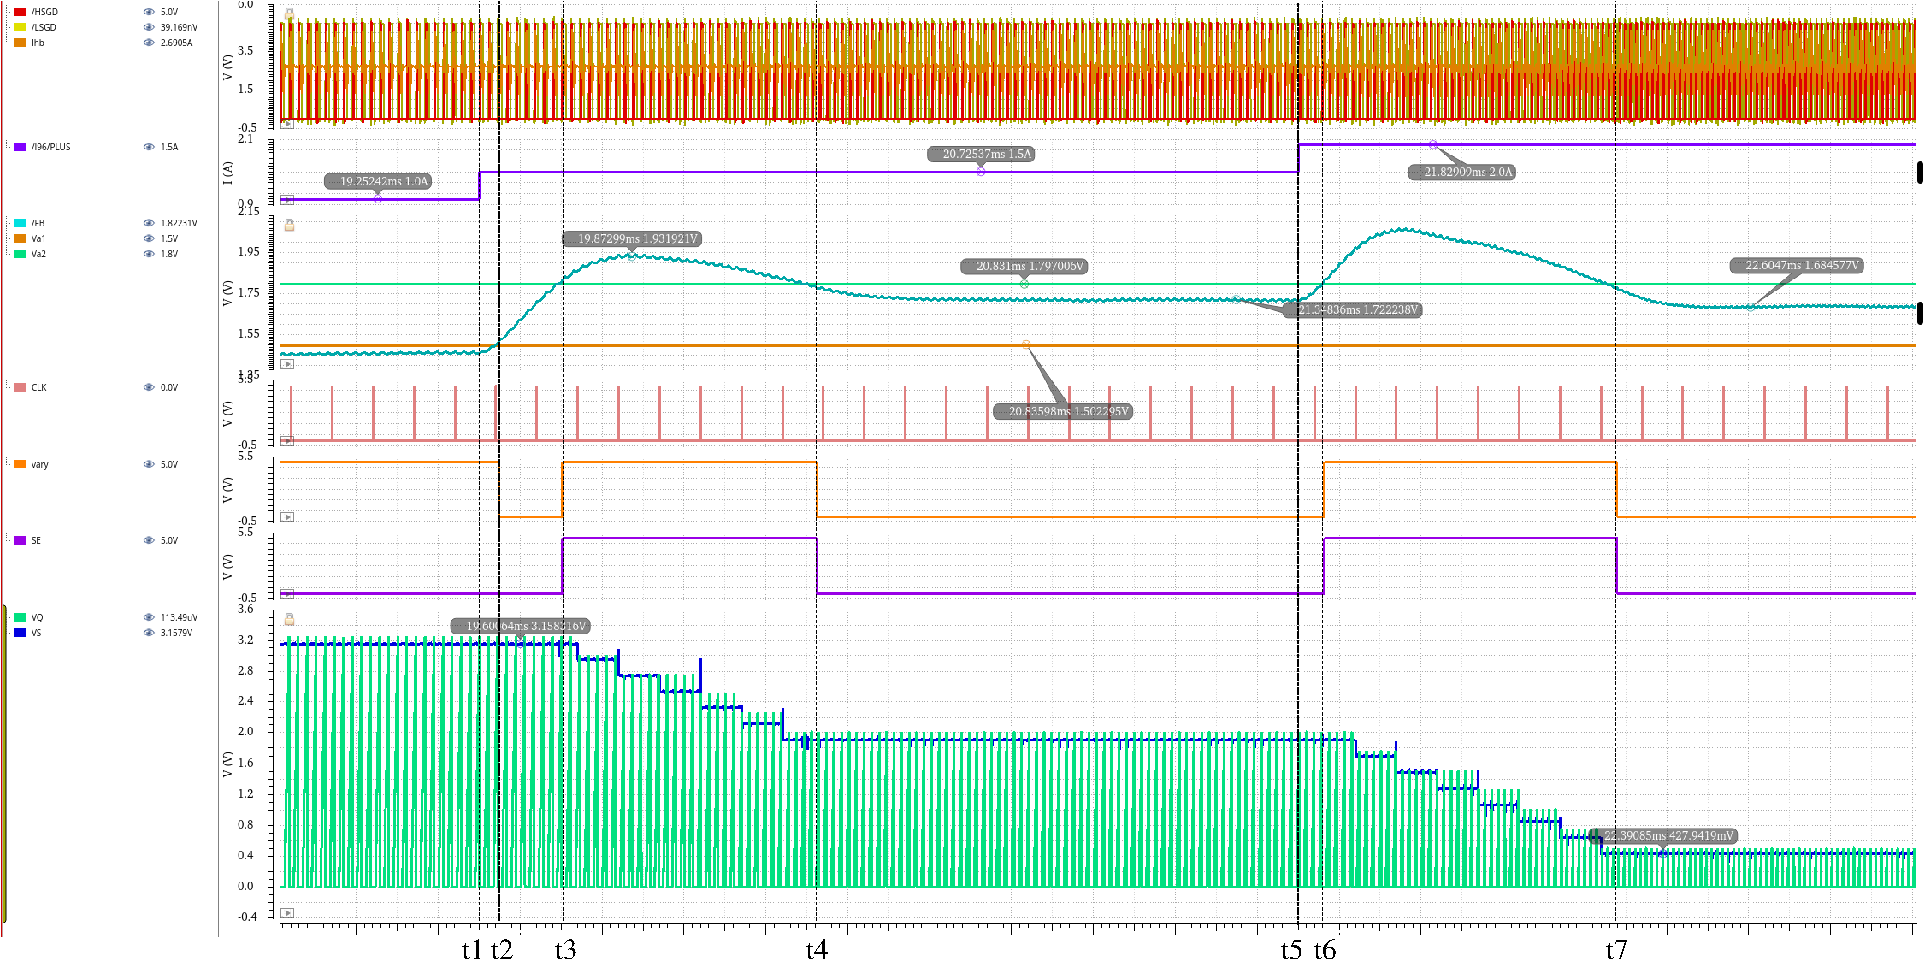
\includegraphics[width=0.8\linewidth]{figures/valley_lock1.pdf}
    \caption{多周期谷值锁定电路波形图}
    \label{fig:多周期谷值锁定电路波形图}
\end{figure} 

图~\ref{fig:谷值锁定放大仿真图}是具体不同负载下谷值锁定电路的仿真波形图。当系统在1.5A的负载电流下稳定后,如图~\ref{fig:多周期谷值锁定电路波形图}中的t4-t5时间段内,谷值锁定电路将每个开关周期内等待时间的谐振谷锁定在相同数值,防止跳谷现象的发生,在图~\ref{fig:谷值锁定仿真图1}中可见得,连续5个开关周期内都保持在第八个谐振谷底处导通低边功率管,未发生跳谷现象。在图~\ref{fig:谷值锁定仿真图2}中可,在2A的负载电流情况下,稳定后的系统在每个开关周期内的第二个谐振谷底处导通低边功率管,同样未发生跳谷现象。根据上文的仿真图可得,谷值锁定电路完成设计的功能,达成了预期的设计指标。

\begin{figure}[htbp]
	\centering
	\subcaptionbox{1.5A负载\label{fig:谷值锁定仿真图1}}{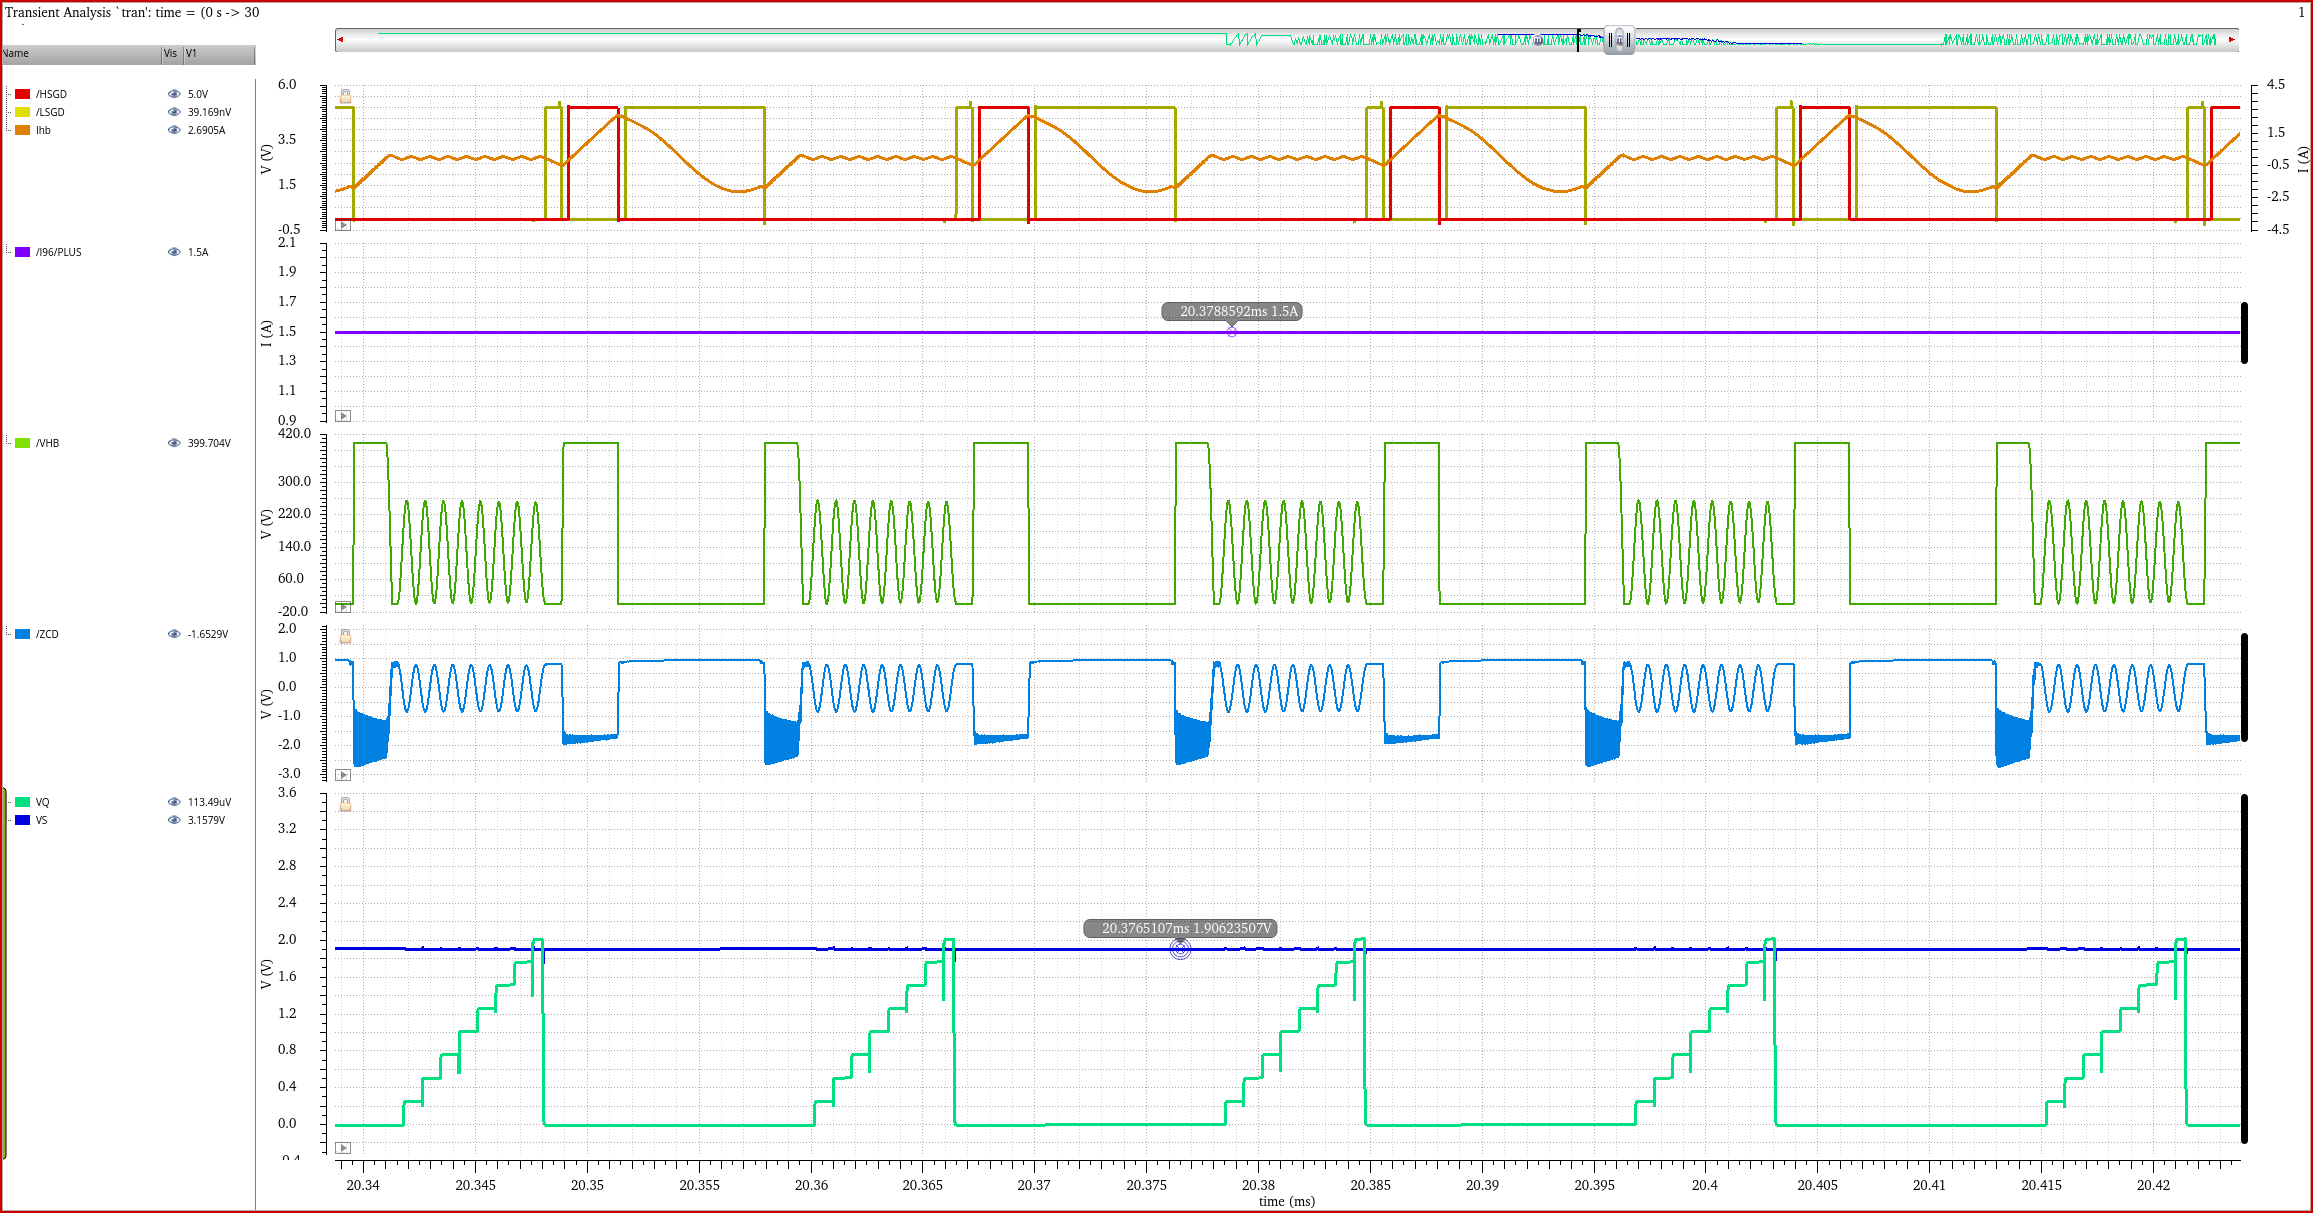
\includegraphics[width = 0.45\linewidth]{figures/valley_lock1.5A.png}}
	\subcaptionbox{2A负载  \label{fig:谷值锁定仿真图2}}{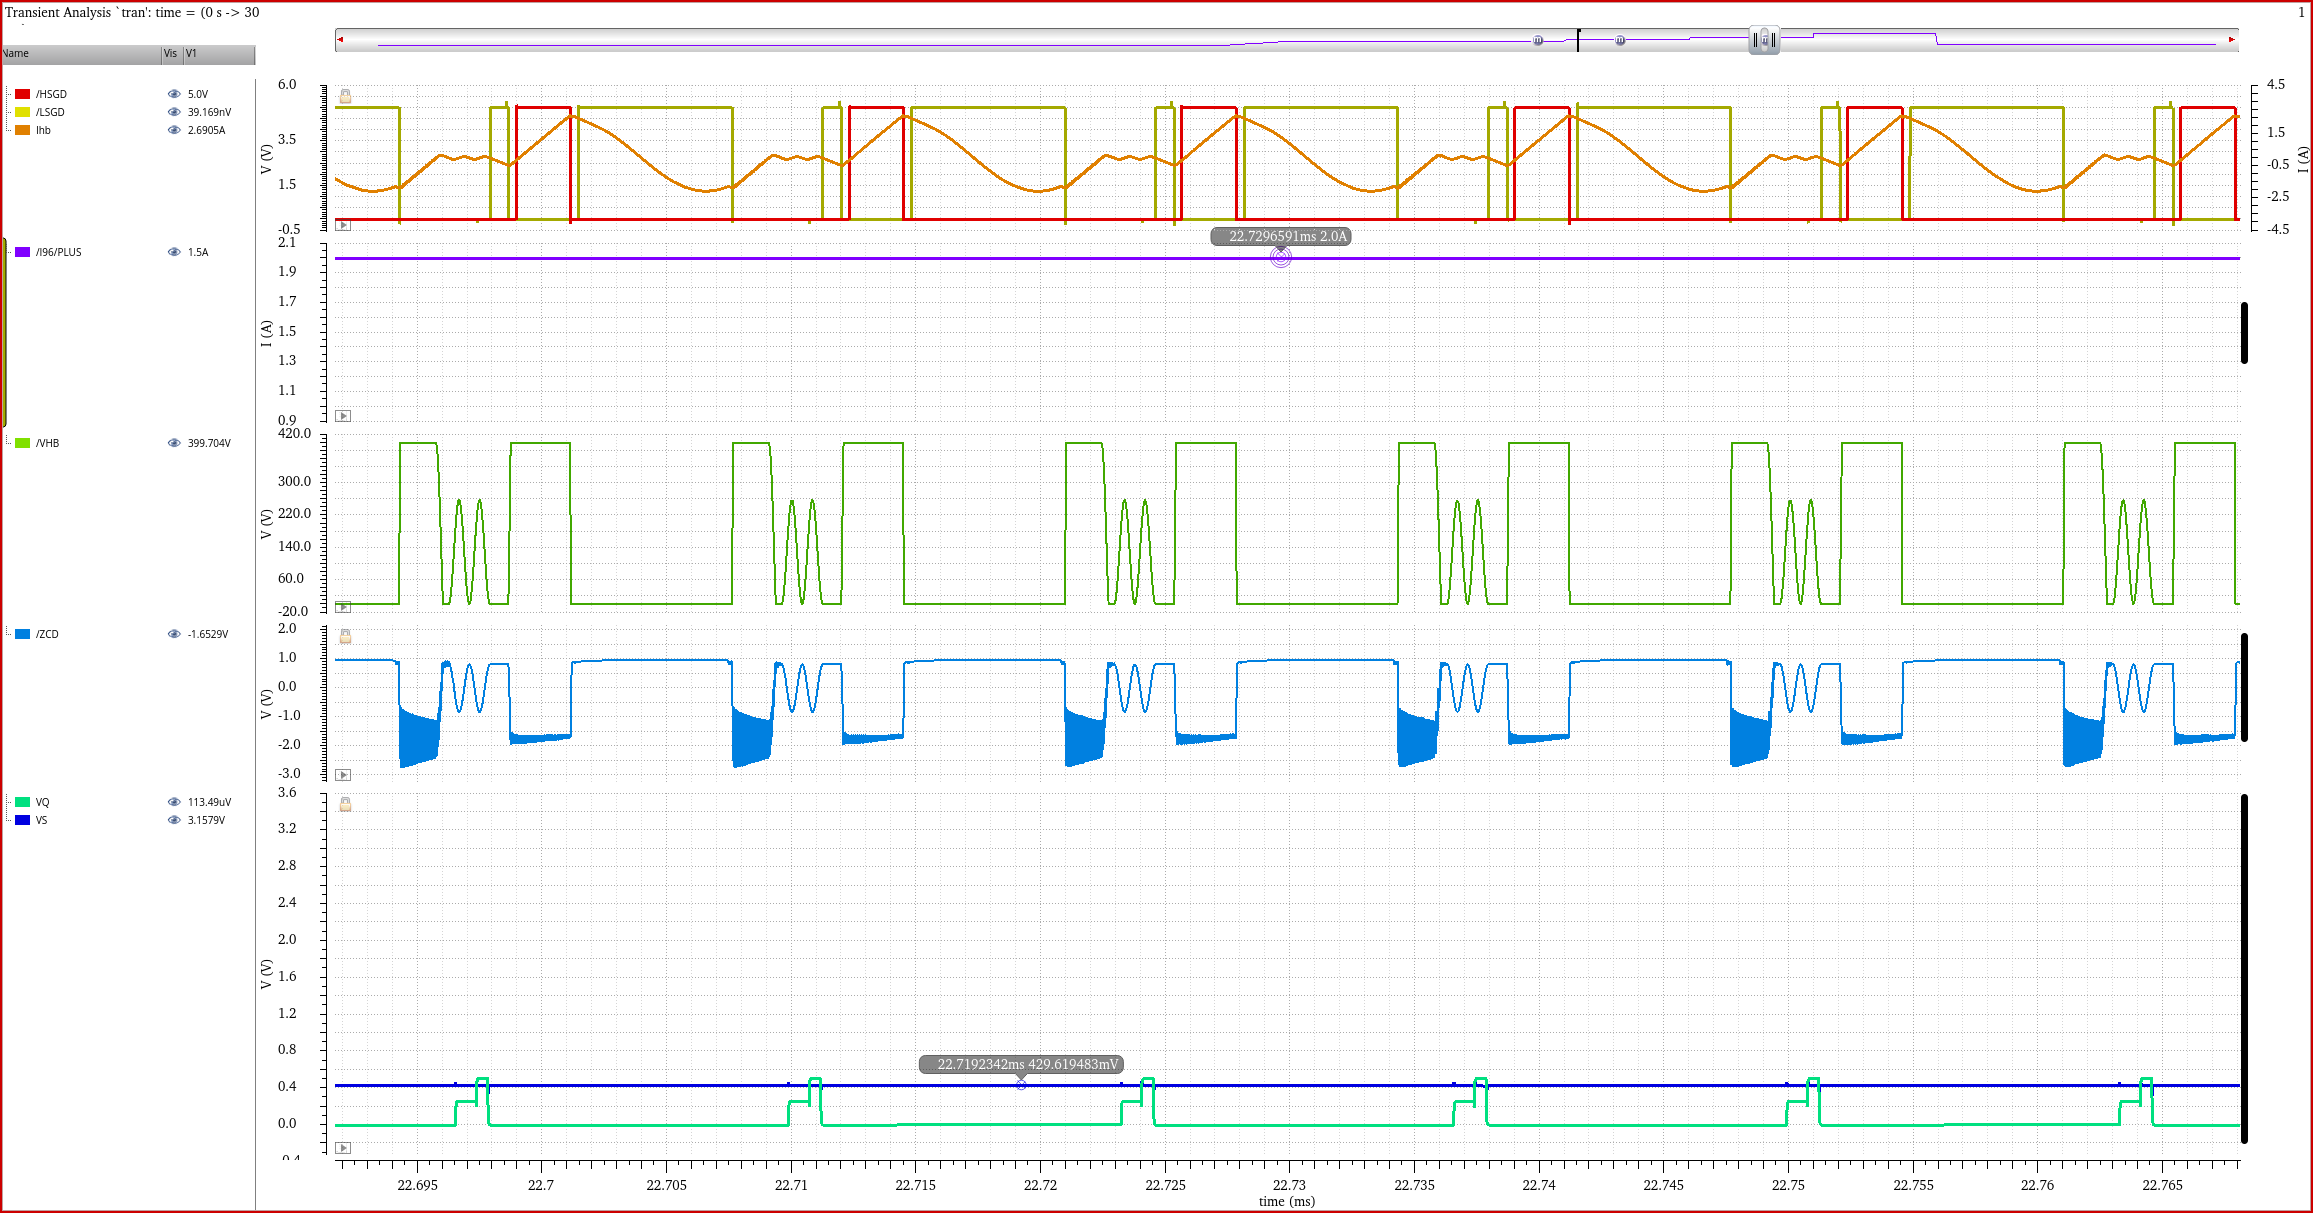
\includegraphics[width = 0.45\linewidth]{figures/valley_lock2A.png}}
	\caption{不同负载谷值锁定仿真图}
	\label{fig:谷值锁定放大仿真图}
\end{figure}

\section{退磁时间动态校准电路}

\subsection{退磁时间动态校准电路原理}

根据上文对~\ref{sec:退磁时间动态校准技术}小节中提到的退磁时间动态校准技术的分析,为了实现高效率的能量传递,应合理的调整低边功率管的导通时间,力求让导通时间和励磁电感的退磁完成时间尽可能的接近。

退磁完成时间会受到多方面因素的影响,如输出电压、输出负载电流、原边峰值电流大小和芯片外围变压器漏感、谐振电容等器件。难以通过计算直接求得退磁完成时间,常规的退磁时间设定技术是通过将退磁时间和输出电压联系起来,采用开环电路控制低边功率管的导通时间。但当输出负载发生波动或外围器件采用不同参数配置时,开环的电路无法对每种情况都匹配,实现最大的能量传递。故本文通过如图~\ref{fig:退磁时间1}中所示的退磁时间动态校准技术完成闭环设计,实现最高的能量传递效率。

\begin{figure}[htbp] 
    \centering
    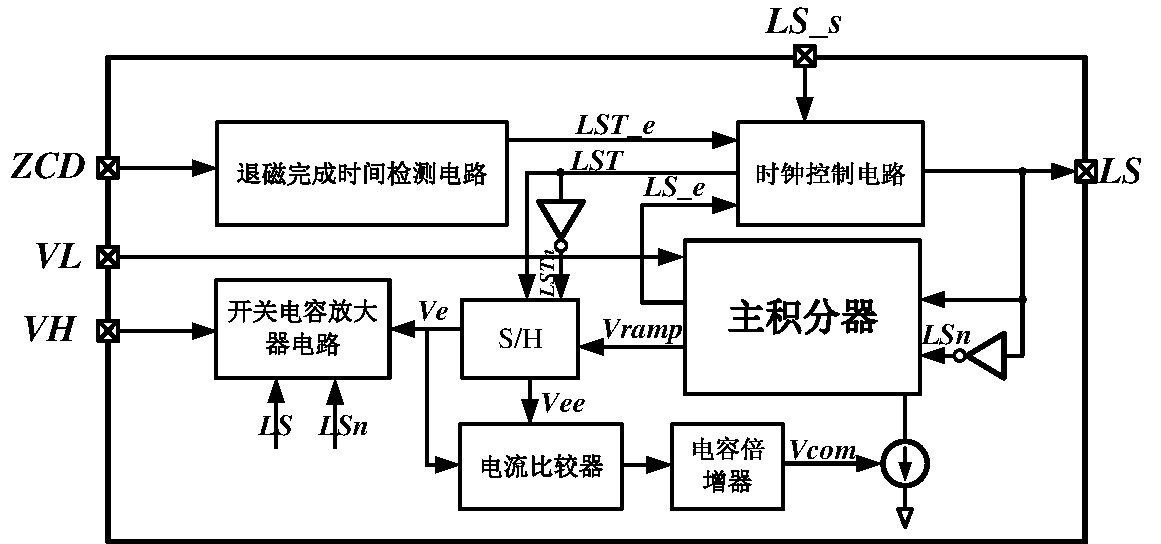
\includegraphics[width=0.8\linewidth]{figures/退磁技术框图.pdf}
    \caption{退磁时间动态校准电路框图}
    \label{fig:退磁时间动态校准电路框图}
\end{figure} 

图~\ref{fig:退磁时间动态校准电路框图}中所示为退磁时间动态校准电路的主要模块框图,主要包括退磁完成时间检测、时钟控制、主积分器、开关电容放大器、电流比较器和电容倍增器等电路。该电路方案通过退磁完成时间检测电路采样得到ZCD引脚电压信号$V_{ZCD}$上的高频谐振信号,输出退磁完成时间结束信号LST\_e,在该信号产生时刻原边电流和漏感电流相交,能量传递结束。但为了防止输出负载微小波动引起的信号LST\_e不稳定情况,不能直接用该信号直接控制低边功率管关断,导致其导通时间的不稳定问题,而是通过动态校准技术延缓变化速度,逐周期逼近到最新的退磁完成时间。

\begin{figure}[htbp] 
    \centering
    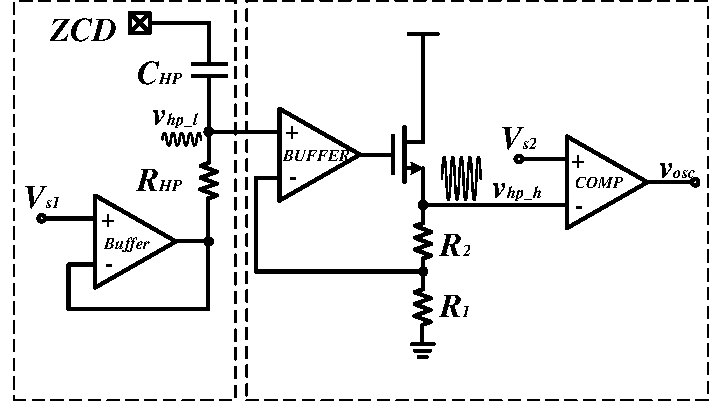
\includegraphics[width=0.6\linewidth]{figures/退磁时间检测电路.pdf}
    \caption{退磁完成时间检测电路}
    \label{fig:退磁时间检测电路}
\end{figure} 

退磁完成时间检测电路的如图~\ref{fig:退磁时间检测电路}中所示,包括高通滤波电路和小信号放大电路,高通滤波电路输入端连接$V_{ZCD}$电压信号,高通滤波模块由$C_{HP}$和$R_{HP}$组成,用于将$V_{ZCD}$电压信号上的微小高频谐振信号采样到给定电压$V_{s1}$上得到电压信号$V_{hp,l}$,再经过弱信号放大模块放大后得到电压信号$V_{hp,h}$,$V_{hp,h}$与给定电压$V_{s2}$通过比较器进行比较,得到输出的退磁完成时间结束信号LST\_e,触发时钟控制电路生成控制信号LST。信号LST不能直接用于控制低边功率管,后续通过图~\ref{fig:退磁时间动态校准电路框图}中其他电路组成的动态校准闭环补偿结构产生功率管实际关断信号LS\_e,通过时钟控制电路生成逻辑控制信号LS去控制低边功率管的导通时间。

\begin{figure}[htbp] 
    \centering
    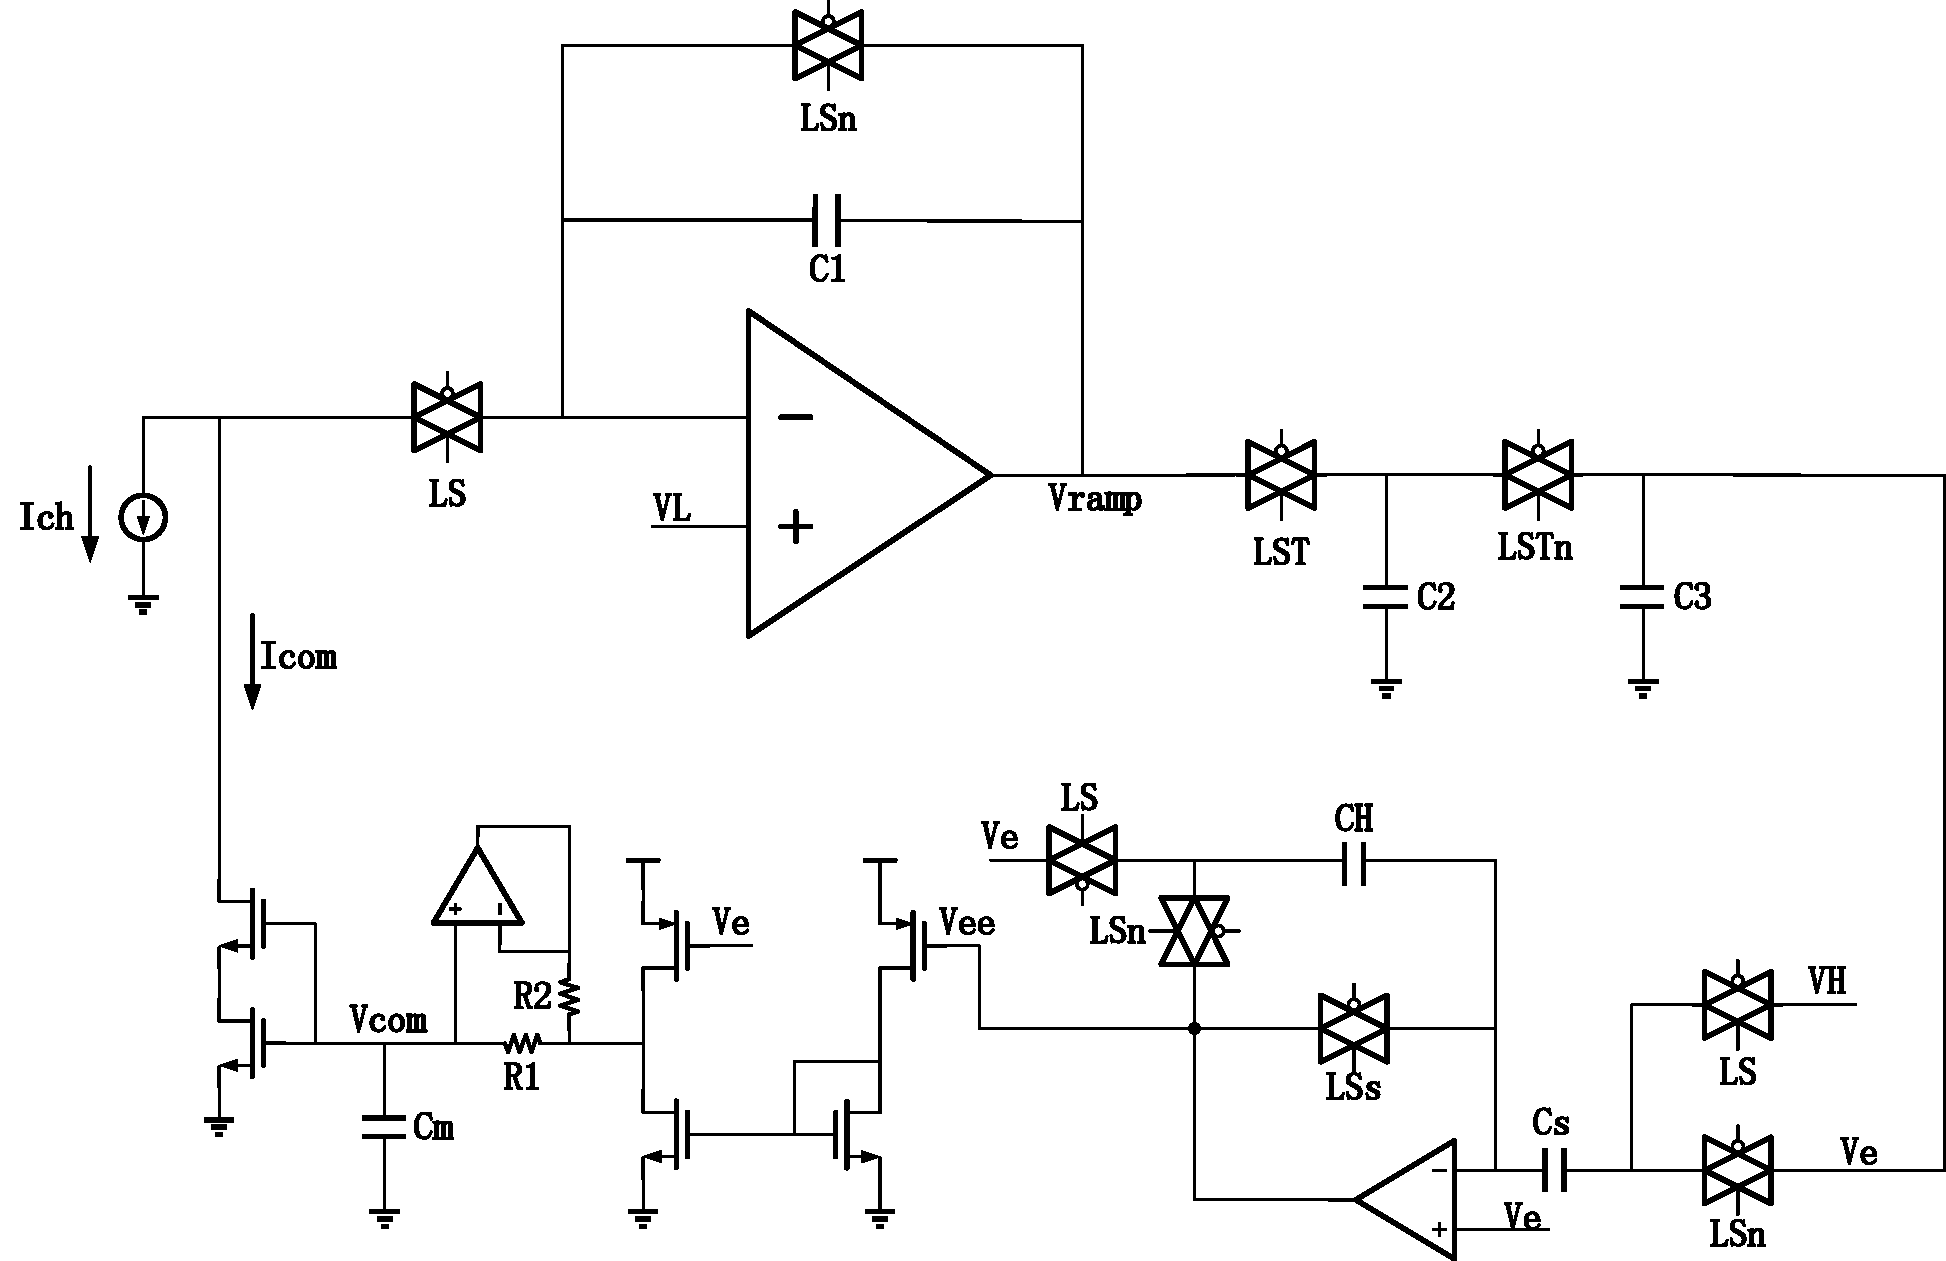
\includegraphics[width=0.8\linewidth]{figures/主积分器环路电路.pdf}
    \caption{动态校准闭环补偿电路}
    \label{fig:动态校准闭环补偿电路}
\end{figure} 

\begin{figure}[htbp] 
    \centering
    \includegraphics[width=0.8\linewidth]{figures/主积分器环路波形图.pdf}
    \caption{动态校准闭环补偿波形图}
    \label{fig:动态校准闭环补偿波形图}
\end{figure} 

图~\ref{fig:动态校准闭环补偿电路}和~\ref{fig:动态校准闭环补偿波形图}分别是动态校准闭环补偿结构的电路图和波形图。该结构的具体工作过程为:

在t1时刻外部输入脉冲信号LS\_s由低电平转为高电平,时钟控制模块输出的时钟信号LS和LST被LS\_s信号触发同样由低电平转为高电平,LS信号开始控制电流Ich对主积分器的积分电容进行充电,输出斜率为k1积分斜坡电压Vramp,LST信号控制采样保持电路采样电压信号Vramp。

电路经过一段时间到达t2时刻,高通滤波采样放大电路检测到外部输入电压信号VZCD的高频谐波振荡,产生脉冲信号LS\_e使得时钟控制电路将时钟信号LST由高电平拉低到低电平,进而将采样电压Ve保持在固定的电压V1处。

在LS为高电平的时间阶段内,开关电容电路同时工作在采样阶段,使得输出电压Vee一直等于前级输入电压Ve,因此后级的电流比较器电路两个PMOS晶体管栅极电压保持相等,Ie和Iee近似相同,没有多余的电流对后级的大电容进行充放电,电容电压Vcom维持不变,由NMOS构成的VCCS也不产生补偿电流Icom改变主积分器电路输出积分斜坡电压Vramp的斜率。

直至电路工作到t3时刻,主积分器积分斜坡电压Vramp大于给定固定电压VH,产生脉冲LS\_e使得时钟控制电路控制时钟信号LS由高电平拉低为低电平,开关电容放大器电路改变为保持放大模式,将输出电压Vee放大到固定电压V2处;此时开关电容放大器电路输出电压Vee大于采样保持电压Ve,电流比较器输出的电流Ie大于Iee,开始为后级电容倍增电路产生的大电容进行充电,电压Vcom逐渐增大,经过VCCS后产生的补偿电流也Icom逐渐增大。

电路继续工作到t4时刻,外部输入的脉冲信号LS\_s再次由低变高,电路进入下一周期,由于上一周期产生的补偿电流Icom增大到一定值,因此本周期主积分器输出的积分斜坡电压Vramp的斜率增大到k2,由于斜率增大,斜坡电压Vramp将更快的大于给定固定电压VH,使得时钟控制电路产生的时钟信号LS相较于前一周期更短,更接近时钟信号LST的脉宽长度。

电路经过与前一周期同样的工作流程后,电压信号Vcom再次在LS信号为低电平时逐渐增大,补偿电流Icom也相应增大,进而控制下一周期的积分斜坡电压Vramp继续增大,时钟信号LS进一步缩短,逐步逼近时钟信号LST。

\subsection{退磁时间动态校准电路仿真分析}


\begin{figure}[htbp] 
    \centering
    \includegraphics[width=0.8\linewidth]{figures/退磁时间技术仿真图.png}
    \caption{退磁时间动态校准电路波形图}
    \label{fig:退磁时间动态校准电路波形图}
\end{figure}

退磁时间动态校准电路的具体波形图如图~\ref{fig:退磁时间动态校准电路波形图}所示。










\section{逻辑控制电路}

\section{保护电路}

\section{系统整体仿真}

• 满载下输出电压纹波仿真

• 恒流模式仿真

• 恒压下20V\_5A、20V\_3A、20V\_1A、5V\_5A、5V\_3A、5V\_1A的仿真图

• 恒压下极轻载的仿真测试BM模式

• 恒压下负载跳变的仿真



\section{小结}





\chapter{版图与后仿}

\section{版图设计规则}
%本文采用 BCD 工艺,B、C、D 分别指 bipolar 双极型晶体管、CMOS 场效应晶 体管、DMOS 双扩散场效应晶体管。BCD 工艺内含高低压 MOS 管、LDMOS、NPN 和 PNP 管、肖特基二极管、金属电阻、多晶电阻等器件,同时包含双极型器件和场 效应管的优点,将高压器件低压器件整合到一起,方便了设计者的使用,其低能耗高 效率、高强度、高耐压、开关高速化等特点使得 BCD 工艺成为目前集成电路设计的 常用工艺。由于大部分集成器件在实际生产中是存在偏差和失配的,成因来自于工艺 尺寸、掺杂等器件参数变化、接触电阻、应力梯度等许多因素,通过在设计中遵守版 图设计的匹配规则、合理规划版图设计可以有效提高电路的精度和性能。 提高器件的匹配性是版图设计的一个重点。电阻常因材料温度系数引起的热变化 和热电效应的影响出现误差。多电阻的匹配一般通过共质心版图技术减小热变化影响, 每个电阻拆成偶数个分段阵列并采用叉指结构摆放,每段电阻应避免长度过短而引入 过大的接触电阻误差以及宽度过窄引起的工艺误差。热电效应是由于电阻接触孔处不 同物质的接触会产生接触电势差,其受到温度变化的影响较大。将电阻叉指结构处理, 电阻段一半沿一个方向连接,另一半沿另一方向连接可消除分段热电势。电阻接触孔 分布的位置应靠近。除此之外匹配度要求高的电阻两端加入 dummy 器件可提高匹配 性,与电阻无关的导线避免从匹配电阻上跨过以减小失配等。 MOS 管是模拟电路设计中常见的高匹配度要求的器件。一般采用共质心的版图 布局,将 MOS 管分成多段,需要匹配的器件叉指并行摆放。除此之外保证 MOS 管 摆放方向一致、尽量紧凑匹配 MOS 管的版图、加设 dummy 管、匹配度要求高的晶 体管远离功率模块等方法可以提高 MOS 管的匹配性。 版图中走线规划对版图优化效果也很明显。如数字模块和模拟模块的地线需要分 开防止串扰。布局中避免时钟线和信号线交叠。对于容易受到干扰的重要信号线加设 隔离保护并远离噪声模块。走线使用高层金属可承受更大电流。地线和电源线上均匀 而大量地打孔用以保证良好接触。走线不宜过长避免引起天线效应。除此之外,对版 图模块合理规划,数字模拟模块之间加入隔离,匹配精度要求高的模块远离功率大的 热源模块等方式都可以提高版图的可靠性[40]。 本芯片采用 Nuvoton 0.35μm 高压工艺完成整体电路版图如图 5.12 所示。版图面 积为 920μm×860μm,包含六个 PAD:VDD、GND、CTRL、FB、GATE 和 CS,版图 通过了 DRC、LVS 验证。

版图设计规则是在集成电路(IC)设计过程中用来指导版图设计的一系列规定和约束。它们旨在确保最终的版图设计满足性能、可靠性和制造要求。这些设计规则将负责电路设计的工程师和负责工艺的工程师联系了起来。制定这些版图设计规则是为了将设计的版图进行标准化,在保证电路可靠性的基础上,利用设计规则尽可能减小芯片版图的面积。版图设计规则的重要性在于确保集成电路(IC)设计在实际制造过程中能够被准确重现。确保设计的顺利实施、产品的高性能和可靠性,以及设计成本的控制。通过遵守规则,设计团队可以更好地实现设计目标,提高产品质量[43],推动IC设计的进步和创新。在实际的IC设计中,不同的工艺以及不同的厂商使用的设计规则往往不同,在版图绘制过程中,常用的设计规则主要包括:

1、线宽和间距规则:规定了不同金属层或多晶硅层中导线的最小宽度和最小间距。这些规则通常由工艺技术能够实现的最小特征尺寸和工艺容忍度所决定。

2、接触孔规则:规定了不同层之间的接触孔的最小尺寸和间距,以确保层与层之间的连接正常进行。

3、阱孔规则:规定了用于隔离衬底和金属层之间的阱孔的尺寸和间距。

4、悬空金属规则:规定了悬空金属结构的最小尺寸和支撑要求,以确保金属线的稳定性和可靠性。

5、器件尺寸和布局规则:规定了器件的最小尺寸、引脚位置和布局要求,以确保器件功能和性能的正常表现。

6、电源线规则:规定了电源线的宽度和间距,以确保提供足够的电流和降低电阻。

7、设计规则检查(DRC)规则:规定了版图设计需要满足的几何和拓扑约束,以便进行自动化的设计规则检查。

8、特殊工艺规则:针对特殊工艺步骤(如电池区域、ESD保护区域等)制定的特殊版图设计规则。

版图设计规则的重要性在于确保集成电路(IC)设计在实际制造过程中能够被准确重现。确保设计的顺利实施、产品的高性能和可靠性,以及设计成本的控制。通过遵守规则,设计师可以更好地实现设计目标,提高产品质量[44],推动IC设计的进步和创新。

\section{版图设计流程}

\section{具体版图设计}

根据版图的设计流程,首先将模块进行划分,然后进行布局连线,本文设计的非对称半桥反激式变换器芯片主要有带隙基准模块、逻辑控制模块、输出驱动模块等构成。完整的版图包括数字模块和模拟模块以及存储一些数字逻辑信号的存储器模块,由于本文主要设计的是模拟部分,所以只展示模拟模块的版图。

\subsection{版图布局}

首先对整个变换器进行版图布局,为了减小数字信号逻辑切换产生的衬底耦合问题,将数字模块和模拟模块进行分开布局,对于模拟部分,本文设计了16个输出通道,为了保证通道之间相互匹配,将16个输出通道对称放在左边,其余模块放在右边,下方为数字部分的版图,因此本文设计的恒流驱动芯片总体布局如图所示。

\subsection{各个模块版图}

\subsection{整体版图}


\section{小结}





% \include{chapters/cp4}
% \include{chapters/cp5}
% \include{chapters/cp6}


\iffalse
% xdus 已经实现下面文件的引用
% 为了使语法提示正确工作,在这里引用但是不编译
%随着全球科技的迅速发展,电子设备的智能化程度随着集成电路产生的发展也越来越高,在日常生活在,开关电源作为各种电子产品的核心模块也愈发的被社会所重视。随着芯片的发展,各种软件层出不穷,但电池材料的发展不够迅速,大众对充电器的功率和充电速度的要求日益提高。反激式AC/DC开关电源变换器由于其隔离性能优异、设计简单和成本较低等因素活跃于中低功率的快充领域。但由于其损耗较大和开关频率较低的特性已逐渐跟不上电子设备的发展,为了满足社会日益旺盛的需求,探索更多的反激式变换器的可能性,本文设计了一款基于非对称半桥拓扑结构的反激式开关电源变换器芯片用于中等功率环境的快充领域。

%本文设计的基于副边反馈结构的非对称半桥反激式变换器芯片,通过多种工作模式在全负载范围内都可以实现功率管的零电压导通,极大地降低功率管的开关损耗,提高电路的转换效率。采用最适配非对称半桥反激式变换器的谐振谷值开关(RVS)模式,在轻载工况下同时实现高低边功率管的零电压导通,新颖性的设计了精确谷底导通模块在谐振谷最低点导通低边功率管,实现最小的开关损耗的同时降低采样电压的导通过冲问题。还设计了退磁时间动态校准模块,实现了原边电感最佳能量的传递并完成了副边二极管零电流关断降低导通损耗,进一步提高电路的转换效率。此外芯片还加入了谷值锁定电路防止出现跳谷问题引起的开关频率波动等不稳定问题,加入峰值电流控制电路实现宽范围输出下副边反馈电压的稳定,满足片内多种电路的控制要求;加入


Millimeter-wave radar point cloud imaging technology plays a significant role in fields such as autonomous driving, medical imaging, and terrain mapping. Radar target point detection and multi-point cloud registration are crucial steps in its application. Due to the low working frequency and high noise interference of millimeter-wave radar, its point clouds are characterized by low resolution, sparsity, and uneven density distribution. These characteristics lead to ineffective detection of millimeter-wave radar target points and difficulties in precise registration of multiple millimeter-wave radar point clouds. This thesis focuses on millimeter-wave radar point cloud detection and registration. Based on the features of millimeter-wave radar range-Doppler maps and the multi-scale neighborhood features of multiple millimeter-wave radar point clouds, this study explores millimeter-wave radar target point detection schemes and precise registration schemes for millimeter-wave radar point clouds, effectively improving the accuracy of target point detection and the precision of multi-millimeter-wave radar point cloud registration.

Addressing the issue that the Constant False Alarm Rate (CFAR) algorithm cannot effectively detect target points under low signal-to-noise ratios and multiple target scenarios, this thesis proposes a Distance-Doppler map target point detection scheme based on Residual Neural Networks, named RA-CFAR. Through extracting global features from distance-Doppler maps using multi-layer residual blocks for global noise assessment, this scheme introduces a self-attention module to capture the spatial location relevance of the peak areas in the distance-Doppler maps, overcoming the sidelobe effects of target point locations within the maps. Comparisons with CA-CFAR、SOCA-CFAR、GOCA-CFAR and OS-CFAR on public datasets and proprietary datasets demonstrate that, in low signal-to-noise ratio scenarios, the Area Under the Curve (AUC) values increased by 4\%, 8\%, 11.9\%, and 29.4\% respectively; in multi-target scenarios, the AUC values increased by 2.2\%, 2.71\%, 3.36\%, and 7.19\% respectively.

In response to the problem of ineffective point feature extraction and the inapplicability of features extracted in denser areas of point clouds in sparser areas, this thesis proposes a feature extraction scheme based on multi-scale neighborhoods. In the preprocessing stage, a KD-tree is introduced to calculate nearby points within the neighborhood to assist in fitting the plane of the point cloud neighborhood. The fitted plane's normal vector is used as the point cloud's normal vector to enrich neighborhood information. During the feature extraction stage, to improve the applicability of features in different sparse regions, features are extracted and combined as point characteristics on multiple neighborhoods of different $\tau$ sizes, integrating Doppler information, fitted normal vectors, and spatial coordinates. In the registration phase, feature distance replaces spatial distance to enhance the robustness of the registration algorithm. Global features are used to estimate initial registration values, and registration parameters are optimized after each iteration to avoid issues with registration convergence caused by improper initial value settings. Experimental results demonstrate that, compared to similar schemes, the proposed solution has reduced RMSE(R), MAE(R), RMSE(T), and MAE(T) by 2.2\%, 8.9\%, 20.9\%, and 35\%, respectively.

The research content discussed has been experimentally validated on public millimeter-wave radar datasets and proprietary datasets through evaluation metrics such as detection rate and registration loss rate. The results indicate that the millimeter-wave radar point cloud registration scheme proposed in this thesis exhibits excellent performance in scenarios with low signal-to-noise ratios, multiple targets, sparsity, and uneven density distribution.
\begin{center}
    {
    \zihao{-4}
    \renewcommand{\arraystretch}{1.28}
    \begin{tabular}{p{4cm}l}
        符号 & 符号名称 \\
        $A$ & 安培 \\
        $mA$ & 毫安 \\
        $\mu A$ & 微安\\
        $dB$ & 分贝 \\
        $Hz$ & 赫兹 \\
        $K\varOmega$ & 千欧 \\
        $ns$ & 纳秒 \\
        $\mu s$ & 微秒 \\
        
    \end{tabular}
    }

\end{center}


\begin{center}
{
\zihao{-4}
\renewcommand{\arraystretch}{1.28}
\begin{tabular}{p{2.5cm}p{6cm}l}
    缩略语 & 英文全称 &  中文对照 \\
    AC &  Alternating Current& 交流电\\
    DC &Constant False Alarm Rate &直流电\\
    CCM & Convolutional Neural Network & 连续导通模式 \\
    DCM & Cell Under Test & 断续导通模式\\
    BCM & Fast Fourier Transform & 临界导通模式 \\
    PWM & Frequency Modulated Continuous Wave & 脉冲宽度调制 \\
    PFM &  Greatest of CFAR & 脉冲频率调制\\
    PSM & Intermediate Frequency & 脉冲跳周期调制 \\
    RVS & Resonance Valley Switch & 谐振谷值开关模式\\
    AHBF& Asymmetric Half Bridge Flyback& 非对称半桥反激式\\
    PSR&  Primary Side Regulation & 原边反馈\\
    SSR &  Secondary Side Regulation & 副边反馈\\
    QR & Quasi-resonant & 准谐振\\
    ACDC &  Residual Attention CFAR & 残差自注意力恒虚警率\\
    DCDC & Root Mean Square Error & 均方根误差\\
    DRC & Design Rule Check & 设计规则检查\\
    LVS &  Layout Versus Schematic & 网表一致性检查\\
    LED & Leading Edge Blanking & 前沿消隐\\
    LST\_e &  & 退磁完成时间结束信号 \\
    LS\_e  &  & 功率管实际关断信号 \\

    
\end{tabular}
}
\end{center}
\section{基本情况} \anon{杨林森},\anon{男},\anon{河北张家口人},\anon[XXX ]{1998年1月出生},\anon[XXX ]{西安电子科技大学}\anon[XXX ]{广州研究院}\anon{集成电路工程}专业2022级硕士研究生。 
\section{教育背景}
\begin{edubg}
\anon{2017.09~2021.07} & \anon{华北理工大学大学},本科,专业:\anon{电子科学与技术}\\
\anon{2022.09~ }& \anon{西安电子科技大学},硕士研究生,专业:\anon{集成电路工程}\\
\end{edubg}
\section{攻读硕士学位期间的研究成果}
\subsection{申请(授权)专利}
\begin{resresult}
	\item \anon[(第一学生发明人)]{袁嵩, \textbf{\anon{杨林森}}, 刘启帆等}.一种用于降低开关损耗的精确谷底开关电路:中国, CN202410228018.0
\end{resresult}

\subsection{参与科研项目及获奖}
\begin{resresult}
	\item 国家重点研发计划, 智慧城市云计算平台及服务关键技术研究, 2019.12-2022.11, 结题, 参与。
	\item 国家自然科学基金, 多域物联网系统数据安全关键技术研究, 2023.01-2027.12, 在研, 参与。
	\item 企、事业单位委托项目, 校园安防智慧哨兵系统, 2021.06-2024.07, 结题, 研发负责人。

\end{resresult}



\bibliography{chapters/references}
\fi


\end{document}
